% !TEX options=--shell-escape

\documentclass[a4paper]{report}

\usepackage[margin=2.5cm]{geometry} % set margins
\usepackage{amsmath} % for align
\usepackage{url}
\usepackage{hyperref}
\usepackage{natbib} % citation styling
\usepackage[dvipsnames]{xcolor} % text colors
\usepackage[utf8]{inputenc}
\usepackage{multirow} % merged rows for table
\usepackage[toc]{glossaries}
\usepackage[toc]{appendix} % appendix
\usepackage{pdfpages}
\usepackage{graphicx}
\usepackage{epstopdf}
\usepackage{float} % placement of figures
\usepackage{listings}
\usepackage{listings-rust}
\usepackage{enumitem} % research question enumeration
\usepackage{pdflscape} % landscape


% CODE FORMATTING
\lstset{
    basicstyle=\ttfamily\footnotesize,
    breaklines=true,
    frame=single,
    rulecolor=\color{gray},
    backgroundcolor=\color{white},
    numbers=left,
    numberstyle=\tiny\color{gray},
    keywordstyle=\color{blue},
    commentstyle=\color{green!50!black},
		tabsize=2
	}

% HEADING FORMATTING
\usepackage{titlesec}
\titleformat{\chapter}[display]
{\normalfont\bfseries\Large}{\chaptertitlename\ \thechapter}{20pt}{\Huge}
\titlespacing*{\chapter}{0pt}{-30pt}{20pt}

% PARAGRAPH FORMATTING
\usepackage{parskip}
\setlength{\parskip}{0.5em}
\usepackage{setspace}
\onehalfspacing

% IMAGE PROCESSING
\epstopdfDeclareGraphicsRule{.svg}{pdf}{.pdf}{inkscape -z -D --file=#1 --export-pdf=\OutputFile}
\AppendGraphicsExtensions{.svg}
\graphicspath{ {img/} }

% RESEARCH QUESTION LISTING
\newlist{researchquestions}{enumerate}{1}
\setlist[researchquestions]{
	label=\textbf{RQ\arabic*},
  ref=RQ\arabic*
}

%% Glossary
\makeglossaries
% SHA-2 Terminology
\newglossaryentry{sha2}{
    name={Secure Hashing Algorithm 2 (SHA-2)},
    description={DEFINE ME!}
}
\newglossaryentry{hash function}{
  name={Hash Function},
  description={A cryptographic algorithm that deterministically maps arbitrary-length input data to a fixed-size hash digest, ensuring properties like collision resistance, preimage resistance, and computational efficiency for verifying data integrity and authenticity}
}
\newglossaryentry{hash digest}{
  name={Hash Digest},
  description={Also known as simply "hash", is a fixed-size output produced by a hash function}
}
\newglossaryentry{compression}{
  name={Compression},
  description={A function that combines the current chaining vector and a message block to produce the next state}
}
\newglossaryentry{expansion}{
  name={Expansion},
  description={Preprocessing step where the message block is expanded into a schedule of words for use in hash computation rounds}
}
\newglossaryentry{truncation}{
    name={Truncation},
    description={The process of shortening the final hash digest to a specified bit-length}
}
\newglossaryentry{message}{
  name={Message},
  description={Input data processed by the hash function, padded and divided into fixed-size blocks for hashing}
}

% Vector Types
\newglossaryentry{IV}{
    name={Initial Vector (IV)},
    description={Predefined initial constants, based on hash function used, to initialize the algorithm's state before processing the input message}
}
\newglossaryentry{CV}{
    name={Chaining Vector (CV)},
    description={Intermediate state values created during message expansion, and used as input for processing each given block iteratively}
}

% Cryptanalysis Terms
\newglossaryentry{collision}{
  name={Collision},
  description={A security vulnerability where two distinct inputs produce the same hash digest}
}

\newglossaryentry{differential}{
  name={Differential},
  description={Controlled differences in input messages analyzed to trace propagation through hash rounds}
}

% SMT Terms
\newglossaryentry{smt}{
  name={SMT},
  description={A Satisfiability Modulo Theory (SMT) solver is a tool that determines the satisfiability of logical formulas with respect to combinations of background theories}
}
\newglossaryentry{encoding}{
	name={encoding},
	description={An encoding is a guidance to allow the solver to either reason better or to prune the search space.}
}

% Report Specific Terms
\newglossaryentry{Pure Brute-force}{
	name={Pure Brute-force},
	description={A \textbf{pure/true brute-force} attack is an attack where all possible hash combinations are attempted with no reasoning logic, attempted as is.}
}

\newglossaryentry{Brute-force}{
	name={Brute-force},
	description={A \textbf{brute-force} attack, as used from here on, is an SMTLIB encoding that follows the SHA-2 mathematical algorithm, but does no additional processing or assertion.
	This means the underlying SAT/SMT implementation \textit{may} still use heuristics or othwerise simplify the problem at hand.
	One way to think about this, is as a brute-force guided search.}
}

\newglossaryentry{FS}{
    name={Free-start collision (FS)},
    description={A free-start collision involves finding two messages, either distinct or identical, that produce identical hash digests, where each message utilies its own distinct chosen IV}
}
\newglossaryentry{SFS}{
    name={Semi-free-start collision (SFS)},
    description={A semi-free-start collision involved finding two distinct messages that produce identical hash digests under a chosen IV}
}
\newglossaryentry{STD}{
    name={Standard collision (STD)},
    description={A standard collision involves finding two distinct messages that produce identical hash digests under a fixed initial value. This is the classic collision resistance security property required of cryptographic hash functions}
}



\begin{document}
\title{\textbf{Improving Secure Hashing Algorithm 2 (SHA-2) Collisions Using Satisfiability Modulo Theory (SMT) Solvers}}
\author{Barlik Marcel \\ City St George's University of London \\ marcel.barlik@citystgeorges.ac.uk}
\maketitle


\begin{abstract}
This work presents a detailed analysis on the performance differences among various Satisfiability Modulo Theory (SMT)
solvers in generating collisions for the SHA-2 family of cryptographic hash functions.
The focus of this project was to quantify which SMT solver is most effective at generating collisions for SHA-256,
a widely adopted hash function critical for maintaining data integrity and security of protocols like TLS.
Additionally, the research involved examining different arguments with these solvers, and their effects to the overall solving performance.
Taking inspiration from recent works, I experimented with various encodings and developed my own theoretical differential encoding to enhance SMT reasoning.
These findings provide both a methodological baseline and actionable insights regarding solver effectivness for future research in automated cryptanalysis.
\end{abstract}


\tableofcontents
\setcounter{tocdepth}{3}


\chapter{Introduction}
\section{Domain Problem}
As part of this research project, my goal was to experiment and investigate potential measurable quantified performance differences in SMT solvers and their arguments --
a novel contribution to SHA-2 collisions.
My primary focus within the SHA-2 family is SHA-256.

Since this is an experimental science research project, which looked at different avenues,
some research questions could not be answered declaratively within the timeframe.
As such, no claims have been made that could not be proven.

\subsection{What is a Hash Function?}
\label{ssec:hash-function-basics}
A hash function is a deterministic mathematical algorithm that takes an input, known as the message, of an arbitrary size,
and maps it to a fixed-size output, known as the hash value, digest or checksum.
Hash functions are fundamental in computer science for data integrity verification, password storage, digital signatures and efficient data retrieval in hash tables.

They are designed in a manner to be efficient to compute, but computationally infeasible to reverse-engineer.
In addition to that, they follow the avalanche effect principles -- they are designed so that a minor change in the input propagates a huge output change.

\subsection{Why SHA-2?}
Secure Hashing Algorithm 2 (SHA-2) is a set of cryptographic hash functions published in 2001 by the National Security Agency.
The main security applications are most notably the HTTPS/SSL/TLS protocols, cryptocurrencies such as Bitcoin, PGP, package authentication and more. \cite{wiki:SHA2}

This work will go into an in-depth explanation about SHA-2 in \ref{ssec:sha2-info}.

\subsection{What is a Collision?}
In cryptography, a collision refers to a scenario where two distinct inputs provide the same output.
As desribed by \cite{NIST_SP_800_107} in 4.1, SHA-256 has a collision resistance of $2^{128}$, meaning it is computationally infeasible.
This mathematical strength is why SHA-2 continues to be trusted for critical security applications, despite being developed over two decades ago.
Discovery of a full collision on SHA-2 algorithms would have a critical security impact on billions of users around the globe.

\subsection{What is a Satisfiability Modulo Theory (SMT) Solver?}
A Satisfiability Modulo Theory (SMT) solver is an automated reasoning tool that combines propositional logic with various computer science and mathematical theories.
Given a specific mathematical/logical problem, a SMT checks if there exists a satisfying condition given the constraints.
It is capable of reasoning about potential inputs to deduct potential computational paths -- either represented as trees or graphs depending on the core problem.
Most (but not all) SMT solvers integrate a SAT solver backend, which handles the boolean structure of the problem.
A standard input, widely accepted by many SMT solvers is the SMTLIB format. \cite{SMTLIB}

No additional knowledge in SMT solvers is required for the understanding of this work.

\section{Research Questions (RQs)}
\begin{researchquestions}
  \item \label{rq1} Does using a more effective SMT solver yield better SHA-256 collision results?
  \item \label{rq2} Does using SMT solver arguments yield better SHA-256 collision results?
	\item \label{rq3} How do different encodings impact SHA-256 collision results?
	\item \label{rq4} Do principles of theory defined in \cite{li_2024} work in an SMT, and could they be improved?
\end{researchquestions}

\subsection{Scope Alterations}
These research questions have slightly deviated in order to become more meaningful and deterministic.
All of them have remained closely related.

\cite{li_2024}'s research utilises somewhat complicated theory and representation.
My original research question eagerly wanted to improve on it straight away.
However, after analysing the situation, it proves a very difficult task on its own.
Instead, it has been altered to look at potential theoretical improvements.

\section{Beneficiaries}
This research provides a formal verification; assurance that SHA-2 is still securely
sound in the near-foreseeable future, while pushing the current field boundaries in
SHA-2 SMT collisions, knowledge and benchmarks.
Everyone indirectly is a beneficiary due to how prominent SHA-2 is.
\ref{chap:pdd}

\section{Work Performed}
In order to answer and reason about the research questions, I developed a tool in Rust. \ref{sec:implementation}
Using this tool, and an outlined benchmark methodology \ref{sec:benchmark-methodology}, I was able to visualise graphs to answer my questions. \ref{sec:graphs}

Similarly, I reasoned about potential encodings and created a bit differential representation that could potentially improve on \cite{li_2024}. \ref{ssec:base4-encoding}

\pagebreak
\section{Additional Information}
During this research project, no assumptions have been made on previous works.
When basing on previous research, the claims were taken with caution, until the results could be replicated.
All mentioned and outlined information is correct as of my knowledge, and can be proven or externally verified if necessary.
This ensures validity and corectness for the entirety of this work.

I assume, the reader has basic programming knowledge, knows about data structures and their differences, as well as the concepts of how to operate a Unix-based system to do the bare minimum.
As part of that assumption, the reader should know what the Rust programming language is, and how it differs compared to other low-level languages such as C and C++ in design.

Aside from this, all critical parts for the understanding of this work have been outlined in a readible manner, throughout this paper before they are necessary.


\chapter{Output Summary}
The primary output of this project is a suite of visualised graphs and tables aimed at addressing research questions \ref{rq1}, \ref{rq2}, and \ref{rq3}.
The most substantial output can be found in Section \ref{sec:graphs} with the respective analysis in \ref{sssec:analysis}
Complete output, albeit without analysis, can be found in \ref{sec:full-results}.

As for \ref{rq4} I investigated potential encodings, taking inspiration from \cite{li_2024}'s representation of differences.
My complete encoding theory can be found in \ref{ssec:base4-encoding}.
This is promising, since it should be capable of reasoning fully about differences, including the non-linearity of SHA-2.
Due to time constraints I was unable to develop and benchmark it.

These outputs primarily benefit the community of researchers by providing insight into different SMT tools and their performance.

\section{Software Tool}
A significant output of this project is the software tool, written entirely by me in Rust to facilitate reasoning about the research questions.
This tool serves as a versatile CLI application for generating, benchmarking, and visualising results related to SHA-2 collisions using SMT solvers.
It is designed to be extensible, allowing additional encodings and functionality implementations.

This software tool consists of approximately \textbf{5357} lines of Rust code (as shown by git \texttt{ls-files}). \cite{git_ls_files}
The full codebase can be found on GitHub mentioned in \ref{sec:implementation}, or alternatively in \ref{sec:codebase}.

The intended recipients of this output are primarily researchers in cryptography, computer security, and formal verification looking for templates for their research.
They will benefit from using this tool by having a base to reproduce and build results, as well as to develop new encoding strategies for SMT solvers.

Some screenshots of the output have been provided in \ref{chap:usage-example}.

\section{Open Source Contributions}
While experiencing issues with SMT solvers, namely Bitwuzla, I decided to contribute to external repositories, in order to bring attention to these issues.
More information about my contributions can be found in \ref{sssec:bitwuzla-issues}.

\section{Additional Information}
This report has been written in a manner and terminology to be convertible to a research paper.
Its benefits (if approved) will serve the SMT2025 Workshop. \cite{smt2025}


\chapter{Context}
\section{Report Specific Term Disambiguation}
SMT solvers inherently rely on logical constraints (not pure brute-force), making the distinction between "brute-force" and "guided search" ambiguous.
This is a disambiguation to give meaning and context behind each term.

\glsdesc{Pure Brute-force}

\glsdesc{Brute-force}

\section{Mathematical Notation}
\label{sec:math-notation}
For all mathematical foundation described in this work, the following mathematical representation is in use: \\
$\gg$ represents a shift right (SHR). \\
$\ll$ represents a shift left (SHL). \\
$\oplus$ represents Exlusive Or (XOR). \\
$+$ represents modulo addition.

As common in Computer Science, all examples of iterators start from 0.

\pagebreak
\section{SHA-2 Collisions and Cryptographic Security}
\subsection{Overview of SHA-2}
\label{ssec:sha2-info}
The SHA-2 family, designed by the National Security Agency (NSA) and standardised by NIST in 2001,
comprises six primary hash functions: SHA-224, SHA-256, SHA-384, SHA-512, SHA-512/224, and SHA-512/256.
These algorithms employ the Merkle–Damgård construction with a Davies–Meyer compression function,
differing primarily in digest size (224 to 512 bits), initial values, and round counts (64 for SHA-256, 80 for SHA-512). \cite{NIST_SP_180_4}
SHA-256 and SHA-512 remain widely adopted in TLS, DNSSEC, cryptocurrencies such as Bitcoin, PGP, package authentication and government applications. \cite{wiki:SHA2}

\subsection{Inner Workings of SHA-2}
The SHA-2 algorithm processes input through a series of deterministic transformations governed by its Merkle–Damgård structure.

\subsubsection{Message Processing}
Input messages undergo a pre-processing step to conform to the 512-bit block for SHA-256 (1024-bit block for SHA-512 respectively).
This step is necessary only when converting an input message to a hash digest.
However, this step is mostly irrelevant for automated reasoning tools like SMTs, which directly use arbitrary message blocks to reason about their values.
As such, no additional knowledge is necessary about the preprocessing step.

\subsubsection{Message Expansion}
\label{ssec:sha2-message-expansion}
The pre-processed message only makes up the first 16 words.
Remaining words, $16 \leq i \leq 63$, are expanded based on the mathematical foundation: \\

\begin{equation}
	\begin{aligned}
		s_0 &= (w_{i - 15} \gg 7) \oplus (w_{i - 15} \gg 18) \oplus (w_{i - 15} \gg 3) \\
		s_1 &= (w_{i - 2} \gg 17) \oplus (w_{i - 2} \gg 19) \oplus (w_{i - 2} \gg 10) \\
		w_i &= w_{i - 16} + s_0 + w_{i - 7} + s_1
	\end{aligned}
\end{equation}

\subsubsection{Function Definition}
\label{ssec:sha2-func-definition}
The SHA-2 standard utilises non-linear functions $Maj$ and $Ch$, which introduce diffusion. These are defined as:
\begin{equation}
	\begin{aligned}
		Maj(a, b, c) = (a \land b) \oplus (a \land c) \oplus (b \land c) \\
		Ch(e, f, g) = (e \land f) \oplus (\neg e \land g)
	\end{aligned}
\end{equation}

\subsubsection{Constants and Initialisation}
Each hash function part of the SHA-2 family uses different initialisation vectors (IVs), or otherwise known as H-constants.
These serve as the initial hash values when starting the compression function.
SHA-256 uses fractional parts of square roots from the first 8 primes, whereas SHA-512 uses cube roots.

The round constants, also known as K-constants, are derived from fractional parts of cube roots for the first 64 primes (SHA-256) or first 80 primes (SHA-512).
These aim to break symmetry in message scheduling during modular addition of the compression function.

\subsubsection{Compression Function}
\label{ssec:sha2-compression-function}
Each H-constant updates one of eight 32-bit registers $a$–$h$, often referred as the "working variables", which are part of the 256-bit starting state.

The compression function employs 64 rounds (80 for SHA-512), where for each round, the following are executed:
\begin{equation}
	\begin{aligned}
		\text{Calculate temporary variables} \\
		T_1 &= h + \Sigma_1(e) + Ch(e,f,g) + K_t + W_t \\
		T_2 &= \Sigma_0(a) + Maj(a,b,c) \\
		\\
		\text{Rotate working variables, calculate $a$ and $e$} \\
		h &= g \\
		g &= f \\
		f &= e \\
		e &= d + T_1 \\
		d &= c \\
		c &= b \\
		b &= a \\
		a &= T_1 + T_2
	\end{aligned}
\end{equation}

What is often referred to as a round-reduced model, is simply a compression with less iterations than standard.
The number of iterations of this compression function, is what are often referred to as the number of "rounds" or "steps" of a collision.

For round-reduced models, a lot of K-constants and expanded messages are not required during compression to obtain the hash.
As such, these can be removed from the SMTLIB encoding as they are redundant.

\subsubsection{Finalisation}
After processing all blocks, the final hash concatenates the eight registers' contents.
At this stage, truncated variants trim the output size.
For SHA-256, this produces a 64-character hexadecimal value.

\subsection{Collision Fundamentals}
A cryptographic collision occurs when distinct inputs $M \neq M'$ yield identical digests $H(M) = H(M')$.
Such collisions violate the deterministic uniqueness expected of hash functions, enabling certificate forgery, blockchain double-spending, and data integrity breaches.
As described in \cite{NIST_SP_800_107}, due to SHA-2's collision resistance, a true brute-force collision requires $O(2^{n/2})$ operations for $n$-bit hashes.
Reasoning and analytical attacks, such as \cite{li_2024}, exploit weaknesses with the use of encodings and heuristics, to achieve practical breaks at reduced-rounds.

\subsection{Classification of Collision Attacks}
\begin{itemize}
    \item \textbf{Free-Start Collisions (FS):} Attacker controls both message blocks and initialisation vectors (IVs).
			A collision occurs with either or both the message and/or IV are unique.
    \item \textbf{Semi-Free-Start Collisions (SFS):} Attacker chooses a fixed IV for both messages, while controlling the message blocks.
    \item \textbf{Classical/Standard Collisions (STD):} Attacker controls only the message blocks.
\end{itemize}

\subsubsection{Satisfiability Theory}
\label{sssec:sat-theory}
During my work, I observed that a standard collision is always unsatisfiable for the first 8 rounds.
This is likely because the constants as part of the standard mathematically make this infeasible.
Since there are 8 working variables, it takes exactly 8 rounds for a full rotation of a given variable, therefore from the 9th round onward at least one collision exists, but more likely many collisions exist.
This does not hold true for SFS or FS collisions, which are satisfiable from the very start.

\subsection{History of Collisions}

\begin{table}[H]
\centering
\resizebox{\textwidth}{!}{
	\begin{tabular}{cccccc}
	\textbf{Hash Function} & \textbf{CT}          & \textbf{Rounds} & \textbf{Time} & \textbf{Memory} & \textbf{References}             \\ \hline
	SHA-256                & \multirow{5}{*}{STD} & 18              & practical     & practical       & \ref{fig:sha256_std} \\
					&         & 31 & $2^{49.8}$  & $2^{48}$                     & \cite{li_2024}        \\
					&         & 28 & practical   & - & \cite{christoph_2016} \\
					&         & 31 & $2^{65.5}$  & - & \cite{mendel_2013}    \\
					&         & 24 & $2^{22.5}$  & -                            & \cite{sanadhya_2008}  \\ \cline{2-6}
					& FS & 39 & practical   & -                            & \cite{li_2024}        \\
					& SFS     & 38 & $~2^{19.2}$ & -                            & \cite{alamgir_2024}   \\
					& SFS & 38 & $2^{37}$    & - & \cite{mendel_2013}    \\ \hline
	SHA-512 & STD     & 31 & $2^{115.6}$ & $2^{77.3}$ & \cite{li_2024}        \\
					& STD     & 24 & $2^{22.5}$  & -                            & \cite{sanadhya_2008}  \\ \cline{2-6}
					& FS & 39 & practical & - & \cite{christoph_2016} \\
					& SFS & 38 & $2^{40.5}$  & - & \cite{maria_2014}
	\end{tabular}
}
\caption{Historical SHA-256 and SHA-512 collisions from 2008 to present, including this paper's SHA-256 results for reference.}
\label{tab:historical-collisions}
\end{table}

The pace of progression in this domain have been very slow moving, as can be seen by \ref{tab:historical-collisions}.
Many researchers have attempted finding vulnerabilities since the big crash of MD4 and similarly structured hash functions. \cite{xiaoyun_2004}

\subsection{Security Implications and Mitigations}
The 2017 SHA-1 collision (SHAttered attack) \cite{marc_2017} demonstrated real-world risks, prompting NIST to mandate SHA-2/3 migration for digital signatures.
While full SHA-2 remains secure, reduced-round vulnerabilities highlight the importance of monitoring cryptanalytic advances.

Recent automated reasoning tool driven attacks underscore the role of SMTs in cryptanalysis.
By encoding SHA-2's nonlinear functions and message expansion into SMT constraints,
the tool can efficiently discover collisions with guaranteed certainty.
Automated reasoning tools may also find differential characteristics, previously deemed intractable.

In the event of a full SHA-2 collision, NIST would most likely retire SHA-2 and urge for immediate adoption of post-quantum encryption standards defined in \cite{NIST_PQC_2024}.

\section{Recent Works}
\cite{alamgir_2024} utilised a SAT + CAS approach.
Their claim was that the SAT + CAS solver is capable of better performance as opposed to just a SAT approach.
Despite this, \cite{li_2024} still beat \cite{alamgir_2024}, but interestingly enough both of them used different encodings.
It would be interesting to see how a SMT approach would fare against these, given a combination of both of these encodings.
\cite{alamgir_2024}'s work makes use of a similar notation as \cite{li_2024}.

\cite{flatt_2024} made a direct attack targetting OpenWRT's implementation of SHA-256.
As of my understanding, OpenWRT used only 12 characters out of the total output hash, where full collisions are more probable due to the smaller search space.
The researcher was able to find a full collision for those 12 characters using true brute-force approaches, utilising a tool called HashCat. \cite{hashcat}
However, since this is not a reasoning tool, this can not be advanced any further -- the only possible way would be to utilise more powerful compute,
and would fall into the same category of NP-Hard as SAT solving.

Most interestingly, the researcher utilised GPU compute for their search instead of CPU compute.
As of my awareness, there have been attempts to make a GPU accelerated SAT or SMT solver, but all failed or were outperformed by standard CPU alternatives. \cite{paraFROST}
This work raises a question -- could it be possible to make advances in reasoning tool that utilise GPU compute for cryptanalysis?

\section{SMT Performance Claims}
\label{sec:smt-performance-claims}
\cite{bellini_2024}'s research compared a wider variety of cryptanalysis tools, including SAT, SMT, MILP and CP for multiple different ciphers, permutations and hash functions.
Their winner categorising strategy is described as:
"The best solver for each cipher is the one with the highest number of wins.
The winner of our competition (for every formalism) is the solver that performs best for the highest number of ciphers (more than 20, each from round 2 to 6)."
Their claim is that "In the SMT solvers category, Z3 and MathSAT are always inferior to Yices2, which is thus clearly the best SMT solver in our testing".

As of my knowledge, no research has previously defined the baseline of what SMT solvers are capable of for SHA-2 collisions.
No work has quantatively defined the floor of what is possible by simply doing nothing except stating the problem at hand.
All research papers I read never mentioned any attempt at this, and made no comments if it was even feasible.
It is likely that researchers who used SAT or SMT solvers were only able of getting a few rounds for collisions,
and took this as an implied hard limit without the use of encodings.
This creates the basis for \ref{rq1} and \ref{rq2}, which aims to fill this knowledge gap.

\pagebreak
\section{Compilation Performance}
\label{sec:compilation-performance}
Prior work demonstrates that binaries compiled from identical source code can exhibit performance or
structural differences due to compiler optimizations, build environments, or platform-specific toolchains.
For instance, \cite{ren_2021} showed that non-default optimisation sequences can amplify binary differences,
while \cite{dietrich_2024} highlights the prevalence of non-bitwise equivalence in alternative builds.
Due to this, all of my work attempts to generate performance equivalent artifacts by specifying exact build tools and their respective versions, as taken directly from the source websites (preferably GitHub releases).


\chapter{Method}
\section{Background}
Prior to this work, I never utilised SMTLIB, and only briefly worked with Rust.
I also never learnt anything about the security of SHA-2 or Hash Functions.
This meant that my development journey was steep, and required a lot of research and trial and error.
Despite this, I persevered; learnt topics that were required, read documentation on SMTLIB and Rust, and produced a viable software to answer my research questions.
This section will mention and evaluate my full implementation methodology, benchmarking structure and mathematical encoding basis.

\section{Project Methodology}
During the development of this project I used a Kanban-styled board, split into multiple sprints.
Each sprint consisted of tasks required towards a certain goal/subgoal of the project.
As the project matured and I read more information from articles, research papers and different sources, tasks and their ordering somewhat changed.
The Kanban-board came in handy for tracking these ad-hoc tasks.

Despite keeping everything organised, the scope of the project was too large at hand and required some alterations.
I quickly found out that \textbf{quality} is more important than \textbf{quantity} in research.
Unfortunately, it is quite hard to have accuracy, consistency and quality while working solo on a research project.
Because of this, I stumbled into issues and oversights which I did not realise until later.
Having had someone validate thins as the project went on, some of the traps I fell into could have been avoided.
This gave me a wider understanding of why research is often conducted by multiple people.

\section{Design}
This project builds a binary providing a Command Line Interface (CLI).
Design choices were still undertaken in various manners as described below.

\subsection{Command Line Interface}
Since the project mainly interfaces with SMT solvers, which are all CLI based -- it made no sense to develop GUIs.
Providing a packaged CLI binary allows reusability and shows intention that the code is ready to be used as is for further
research and/or encodings.

For the design of subcommands, I took into consideration what functions were called most often with their respective arguments.
Based on that, I derived default arguments and categorised functionality by subcommand.
All subcommands with their respective arguments can be retrieved by appending \verb|--help| to the command/subcommand invocation.
An image representing this can be seen in \ref{chap:usage-example}.

A Rust crate clap.rs was used for command functionality. \cite{cargo:clap}

\subsection{Graphs}
\label{ssec:graph-design}
Rust has somewhat limited visualisation libraries.
Charming.rs provides very beautiful results, but has very limited control and otherwise uses an extremely heavy JavaScript backend. \cite{cargo:charming}
Plotters.rs on the other hand, is a long standing and time tested visualisation crate,
that gives almost all control over plotting, albeit with very verbose and hard to learn syntax. \cite{cargo:plotters}
Due to the limited choice, I have chosen plotters as my graphing library.

I utilised the SVG backend to render images, using a colour pallette defined for consistency.
Due to some graphs having a lot of relevant data, where up to 10 colours had to be used, some colours simply clash together -- this was inevitable.
My attempt at avoiding this was by ensuring contrasting colours where possible.
No Rust visualisation crates support patterns (such as dashed lines), and utilising Python or alternative options would provide greater complexity,
at the cost of having an extensible bundled software.
Inevitably, some data could not be split, as it would become less meaningful.
Due to this, some graphs might be harder to read.
As an alternative, I have bundled tables in \ref{sec:full-results-tables}, which contain the raw values.

\subsection{Graph Filtering \& Correction}
\label{ssec:graph-filtering-and-correction}
All graph data is verified with the SHA-2 implementation.
Any invalid results are automatically filtered out and removed from all plots.

Due to some issues in my SMTLIB generation code, all satisfiable SHA-512 results are invalid.
As such, the SHA-512 graphs look very empty, despite investing around 30 hours of benchmark runtime.
With the short timeframe to resolve this, I shifted focus towards other experiments.
I make mention of this, since my software is capable of generating SMT for the entire SHA-2 family, given a proper implementation.

\subsection{Understanding Graphs}
In order to answer the research questions effectively, I created 3 different visualisation layouts.

\subsubsection{Comparison Graph}
With the main purpose of providing a side by side comparison of each solver baseline, the comparison graph plots data on a Cartesian2D line graph,
where the compression rounds are displayed on the X-axis and $\log 2$ time on the Y-axis.

The timeout is the top of the graph.
One way to understand this graph is -- the line that goes the most to the right (more rounds), while staying low (less time) is the best.
Additionally, the consistency and linearity of the line provides insight about the reasoning of the problem.

This graph is used to answer \ref{rq1} in \ref{sec:graphs}.

\subsubsection{Baseline Graph}
The baseline graph was designed to primarily reason and compare between different runs with variants.
It utilises a Cartesian2D line graph, plotting a main baseline in the middle.
Any missing or invalid data is skipped from plotting.
Deviation data is then calculated from the baseline based on time difference, and represented as a percentage.

If no plot exists on baseline, but a valid deviation is plotted, $+\infty$ will be used as the deviation value.
This can be interpreted as "This was infinitely faster than the nothing achieved (on baseline) within timeout".
If a baseline exists, but no deviation for that round is present, the plot will be skipped.

A rough run-to-run variance is shown with a grey-ish colour near the middle.
The green area with $-\%$ implies "this took $x\%$ less time, compared to baseline".
Similarly, the red area with $+\%$ implies "this took $x\%$ more time, compared to baseline."

The graph scales with the results, and trims out at 100\% in both directions.
When a result is plotted on the edge of the graph, the deviation is $\geq 100\%$ (i.e. twice as long or half as long).

This graph was written with generics in mind, and was reused to visualise results for \ref{rq2} and \ref{rq3} in \ref{sec:graphs}.

\subsubsection{Detailed Graph}
The detailed graph is more complex in terms of construction.
Unlike other graphs, only a single benchmark run is plotted.
It utilises a DualCartesian2D coordinate system, where the first line graph relates to time taken in $\log 2$, and the second to memory usage in Mibibytes (MiB).

Since SMT solving prefers more locality in memory hierarchy, this graph can help understand if the performance degradation is due to hardware limitations, such as saturating all CPU L3 cache.
A graph for Bitwuzla with additional reruns can be seen in the full results \ref{sec:full-results}.

\pagebreak
\section{Implementation}
\label{sec:implementation}
All code was written in Rust (rustc version 1.85.1), compiled with the provided LLVM backend, and linked with mold (version 2.37.1). \cite{rust} \cite{mold}

The code is licensed under CC BY-NC-SA 4.0, allowing free use with attribution, while limiting any commercial use. \cite{cc_by-nc-sa}

Repository for the code can be found below, with further build information in the README.md file:
\begin{center}
	\url{https://github.com/Supermarcel10/CSG-IN3007/tree/0.1.1} \\
	\textcolor{gray}{\textit{At the time of submission, this repository is private}}
\end{center}

\subsection{Functionality}
The functionality of the tool is split into multiple parts.
Each part is invoked by a separate subcommand.

\subsubsection{SMTLIB Generation}
\label{sssec:smtlib-generation}
The SHA-2 algorithm can be expressed as mathematical operations on a set of bits, where the Theory of Quantifier Free Bit Vector (QF\_BV) is the primary foundation.
This subcommand generates SMTLIB 2.6 files to talk with SMT solvers universally.

At present the code is capable of generating brute-force (purely modelling the SHA-2 algorithm), as well as differential encodings (Subsection \ref{ssec:differential-encoding}).
The generated files can also be written with $Maj$ and $Ch$ simplifications (Subsection \ref{ssec:simplification-encoding}), as well as alternative bitwise add (Subsection \ref{ssec:add-encoding}).
Designed with extensibility in mind, the base 4 encoding (Subsection \ref{ssec:base4-encoding}), which is partially implemented, can be easily added on by appending a new definition.

Rust does offer some SMTLIB based crates. \cite{cargo:smtlib}
However, these mostly interface directly with solvers, and provide no real way to of writing all instructions to a \texttt{.smt2} file.
Because of this, no additional crates were used, and I manually wrote files using \texttt{std::fs} from an owned \texttt{std::String} containing my SMT code.

\subsubsection{Load}
\label{ssec:load}
The \texttt{load} subcommand reads (an) inputted result file(s) from a given dir/file path.

Loaded data is then deserialised into a \texttt{Benchmark} struct.
The struct aims to preserve the original output of console out (cout) and console error (cerr), while storing additional metadata and information.
By doing so, any additional data can be traced back, benchmarks can be reran with known parameters, and filtering is made simple.

One of my objectives mid-way was to migrate to rusqlite, a sqlite wrapper API for Rust. \cite{cargo:rusqlite}
This would allow cleaning up the hundreds of JSON result files, and make querying even easier.
However, in doing so this would hinder the ablity to quickly view a result file without additional tools.
With this consideration, I considered this a very low priority, and put the time aside for more experiments instead.

\subsubsection{SHA-2}
Written with \cite{NIST_SP_180_4} guidelines, this subcommand provides a partially deconstructed SHA-2 implementation.
No established SHA-2 implementations allow control over the number of compression rounds, message digest or Initial Vector.

My original plan was to reuse parts of the Rust sha2 crate. \cite{cargo:sha2}
However, the inner workings utilise dark arts wizardry
\footnote{Rust dark arts refers to "The Dark Arts of Unsafe Rust", defined by The Rustonomicon. \cite{rustonomicon}},
with very optimised system calls based on architecture.
Due to the complexity, I opted for my own implementations from scratch.

This implementation is not formally verified, but outputs the correct hash digest for standard variables against standard implementations.
Due to SHA-2's avalanche effect mentioned in \ref{ssec:hash-function-basics}, this likely means the implementation is fully correct for the hash functions implemented.

My original implementation of SHA-2 utilised generics, and took in a 32 or 64 bit unsigned integer as the word type.
This functioned correctly, and was somewhat simple to build, however was very restrictive.
Having multiple components relying on the SHA-2 implementation, it hindered development by requiring those generics everywhere.
To simplify this, I rewrote the entire SHA-2 functionality to use an enum structure with fields instead.

\subsubsection{Benchmarking}
\label{sssec:benchmarking}
The \texttt{benchmark} subcommand is the primary and most important part of the software.
Given an input of a solver, round range, collision type, encoding and argument matrix, it calls the solver on the host machine and executes it with the \texttt{time} command.

Different SMT solvers output satisfiable (SAT) results in different bases, formats and patterns.
To overcome this, I created a RegEx pattern to detect and process the input for boolean, decimal and hexadecimal.
Additional formats can easily be defined in the \texttt{SmtOutputFormat} enum.

Another challenge was parsing the error codes returned from the SMT binary.
There are no definitive standards related to output status of a solver.
CVC5 as an example, returns an error code if the result is unsatisfiable, whereas some others return a success code.
To overcome this, my output parser utilised the status code and console output to determine benchmark result.

A thread with a chrono timer is spawned right before a benchmark starts.
This has minimum performance overhead, if any at all.
When the thread wakes from sleep, the timeout period has elapsed.
Consequently, the entire process stack is killed with \texttt{SIGTERM} (19), the output parser is ran and a \texttt{Benchmark} struct object is serialised.
Benchmarking continues until all user options have been exhausted.

If the stop tolerance is hit, all benchmarks for the given solver are aborted, and benchmarking moves to the next viable solver (if applicable).
This can happen for multiple reasons.
One example of this, is if a SMT error is encountered.
In such case, my result parser will return a \texttt{SMTError} for its status, and increment the stop hit count.

When a benchmark succeeds at finding a collision, or if no collision exists, the chrono thread is aborted and the parser reads the tokens and creates a new \texttt{Benchmark} object.
This is then verified using the \texttt{sha2} subcommand, and the metadata is attached to the \texttt{Benchmark} struct.
When complete, this is dumped to disk by deserialising the object and freeing memory for the next benchmark.

\subsubsection{Graph Plotting}
The \texttt{graph} subcommand is responsible for regenerating all the graphs from the filtered deserialised data.
For designs and further information, refer to \ref{ssec:graph-design}.

\section{Benchmark Methodology}
\label{sec:benchmark-methodology}
In order to obtain quantifiable results towards answering \ref{rq1}, \ref{rq2} and \ref{rq3} the \texttt{benchmark} subcommand described in \ref{sssec:benchmarking} was used.
This section goes in depth related to the methodologies and strategies employed for consistent, reproducible and reliable data.

A dedicated X86\_64 machine was set up for running this workload, with no background tasks or workers, and an otherwise fresh installation of linux.
Each benchmark run was invoked sequentially (one after the other), as to ensure no performance degradation.
The machine was set up in a manner to provide the most reproducible results.
The default parameters when running were \texttt{--round-range 1..21 --stop-tolerance 0 --continue-on-fail true}.
A timeout period, of 15 minutes (default), was utilised for all benchmarks.
The hardware, parameters and software versions are the basic configuration for all figures presented, unless otherwise specified.

\begin{center}
	\begin{tabular}{|r|c|}
		\hline
		& \textbf{Runner Specification} \\
		\hline
		\textbf{CPU} & AMD Ryzen 9 5900X \\
		\textbf{MEM} & 4 x 32GiB DDR4 3600MHz CL 36 \\
		\textbf{OS} & NixOS 25.05 (Warbler) x86\_64 \\
		\textbf{KERNEL} & Linux Realtime 6.6.77-rt50 \\
		\hline
	\end{tabular}
\end{center}

\subsection{CPU and XMP Configuration}
The primary task of my home lab prior to this research was to run 24/7 as a home server configuration with miscelaneous tasks.
As such, some settings are tailored to lower power draw, better reliability and efficiency.
These settings lock the core clock at base 3700MHz and disable any turbo boost clock.
This reduces performance, but provides more consistent run-to-run performance and result reproducability.

The following BIOS settings have been applied:
\begin{center}
	\begin{tabular}{|r|c|}
		\hline
		\textbf{Setting} & \textbf{Value} \\
		\hline
		\textbf{CPU Clock} & 37.00 \\
		\textbf{CPU Clock Control} & 100.000 MHz \\
		\textbf{XMP} & DDR4-3600 18-22-22-42-64-1.35V \\
		\textbf{CPU Vcore} & 0.818V \\
		\textbf{CPU Vcore Loadline Calibration} & LOW \\
		\textbf{CSM Support} & ENABLED \\
		\hline
	\end{tabular}
\end{center}

\subsection{Kernel Choice}
\label{ssec:kernel-choice}
The runner utilises the Linux Realtime kernel, which aims to have predictable response times.
One of the main differences is the task scheduling and interrupt handling.
In short, the rt kernel uses a preemptible task assignment system, where in most cases high priority tasks cannot be interrupted by the kernel.
Additionally, because of the scheduling, multi-threaded workloads often become slightly more deterministic and reproducible.
This is all at the cost of some throughput loss.

In theory, it would be possible to test the differences between kernel choice, specifically for SMT solving.
My current implementation would fully support this, and could produce a graph specific to answer this question.
Producing a baseline run for all the solvers would take worst-case 40 hours per kernel to generate a graph towards a single SHA-2 hash function.
This means producing data for 3-4 different kernels would take an additional 160 hours of benchmark runtime.

\subsection{Reproducability}
This runner can be rebuilt at any time, using the NixOS configuration found here: \\
\url{https://github.com/Supermarcel10/NixOSConfig/blob/f1d26ec/devices/E01/configuration.nix}

\section{SMT Solver Choice}
\label{sec:smt-solver-choice}
Selecting appropriate solvers for benchmarking is crucial to ensure comprehensive coverage and reliable results.
To achieve this, I aimed to create an exhaustive list of currently available SMT solvers.
The following table lists the solvers tested in this work, along with their versions and corresponding citations:

\begin{center}	\begin{tabular}{|r|c|l|}
		\hline
		\textbf{Solver} & \textbf{Version} & \textbf{Citation} \\
		\hline
		Z3 & 4.13.4 & \cite{z3} \\
		CVC5 & 1.2.1 & \cite{cvc5} \\
		Yices & 2.6.5 & \cite{yices2} \\
		Bitwuzla & 0.7.0 & \cite{bitwuzla} \\
		Boolector & 3.2.3 & \cite{boolector} \\
		STP & 2.3.4 & \cite{stp} \\
		Colibri2 & 0.4-dirty & \cite{colibri2} \\
		MathSAT & 5.6.11 (1a1154baf0ab) & \cite{MathSAT} \\
		\hline
	\end{tabular}
\end{center}

\section{Implementation Challenges}
\subsection{SMTLIB Compatibility}
\label{ssec:smtlib-compatibility}
The current available version of the SMTLIB standard is 2.7.
However, as of writing this report, most of the solvers do not support this version.
Therefore, all encodings and \texttt{smt2} files in this work have been written using the SMTLIB 2.6 standard. \cite{SMTLIB}

Some solvers use an older version of SMTLIB 2.0, which does not provide the `\verb|:left-assoc|` feature.
This would require rewriting a significant portion of the SMT code to maintain compatibility, leading to those solvers being excluded from the benchmarks.

\subsection{Compilation and Linking Issues}
\label{ssec:compilation-linkage-issues}
\subsubsection{MathSAT}
\label{sssec:mathsat-issues}
MathSAT dynamically links to libraries in the binary, which did not work as expected.
To resolve this issue, I patched the ELF file considering its closed-source nature.
Due to reproducability, MathSAT is present in the \texttt{solvers} directory with a \texttt{mathsat\_patch.nix} file.

\subsubsection{Colibri2}
\label{sssec:colibri2-issues}
Colibri2 worked but exhibited some fundamental problems.
It occasionally threw internal errors and sometimes generated output that failed SMTLIB assertions.
This can only be seen in the JSON files part of the codebase.

As mentioned in \ref{ssec:graph-filtering-and-correction}, my graph implementation automatically filtered out invalid results, allowing all Colibri2 results to be included while displaying only valid ones.

\subsection{Solver Issues}
\label{ssec:benchmark-solver-issues}
\subsubsection{Bitwuzla}
\label{sssec:bitwuzla-issues}
Bitwuzla was very strong from the beginning and ran without significant issues.
However, during experimentation, I discovered an issue with memory handling that has since been resolved through creating an issue on their repository (\url{https://github.com/bitwuzla/bitwuzla/issues/169}).

Additionally, I encountered issues with the \texttt{nixpkgs} repository related to compiling the Kissat solver backend.
I submitted a pull request to fix this issue, which has since been merged (\url{https://github.com/NixOS/nixpkgs/pull/400299}).

As mentioned in \ref{sec:compilation-performance}, different tools during compilation can have varying runtime performance.
For benchmarking the Kissat solver backend in Bitwuzla, I used my built binary.
Other backends performed within acceptable variance of the original runs.

\section{Encodings}
\label{sec:encoding}
Each of the encodings, and their combinations were benchmarked.
Their analysis can be seen in \ref{sssec:encoding-analysis}.

\subsection{Simplifying Compression Functions}
\label{ssec:simplification-encoding}
As described in \ref{ssec:sha2-compression-function}, the SHA-2 compression function relies on two non-linear functions:
the choice function \(\textrm{Ch}(e, f, g)\) and the majority function \(\textrm{Maj}(a, b, c)\).
Both functions traditionally employ XOR operations to combine inputs as defined in the SHA-2 standard \cite{NIST_SP_180_4}.
From my mathematical analysis, it is possible to replace XOR with OR in these functions, simplifying their implementation, while preserving logical behaviour.

The original definitions of the functions are:
\begin{equation}
	\begin{aligned}
		Ch(e, f, g) &= (e \land f) \oplus (\neg e \land g) \\
		Maj(a, b, c) &= (a \land b) \oplus (a \land c) \oplus (b \land c)
	\end{aligned}
\end{equation}

In the simplified encoding, all XOR operations were substituted with OR:
\begin{equation}
	\begin{aligned}
		Ch'(e, f, g) &= (e \land f) \lor (\neg e \land g) \\
		Maj'(a, b, c) &= (a \land b) \lor (a \land c) \lor (b \land c)
	\end{aligned}
\end{equation}

To validate equivalence, truth tables were constructed for all possible input combinations.
Table~\ref{tab:truth-table} demonstrates identical outputs for both $Ch$ and $Ch'$, as well as $Maj$ and $Maj'$.
This arises because the sub-expressions in $Ch$ are mutually exclusive: $e \land f$ and $\neg e \land g$ cannot simultaneously be 1.
Consequently, OR and XOR produce identical results in this context.
Similarly, for $Maj$, the OR operation captures the majority condition, as overlapping terms do not affect the final output.

\begin{table}[H]
\centering
\caption{Truth table comparing original and modified $Ch$ and $Maj$ functions.}
\label{tab:truth-table}
\begin{tabular}{ccc|cc|cc}
\(x\) & \(y\) & \(z\) & \(\textrm{Ch}\) & \(\textrm{Ch}'\) & \(\textrm{Maj}\) & \(\textrm{Maj}'\) \\ \hline
0 & 0 & 0 & 0 & 0 & 0 & 0 \\
0 & 0 & 1 & 1 & 1 & 0 & 0 \\
0 & 1 & 0 & 0 & 0 & 0 & 0 \\
0 & 1 & 1 & 1 & 1 & 1 & 1 \\
1 & 0 & 0 & 0 & 0 & 0 & 0 \\
1 & 0 & 1 & 0 & 0 & 1 & 1 \\
1 & 1 & 0 & 1 & 1 & 1 & 1 \\
1 & 1 & 1 & 1 & 1 & 1 & 1 \\
\end{tabular}
\end{table}

The substitution preserves non-linearity, as both OR and XOR are non-linear operations in Boolean algebra.
Diffusion properties also remain unaffected, as the output dependence on input bits is unchanged.

This simplification aims to optimise the reasoning a solver might attempt.
An XOR operation can be expressed using a combination of OR and AND logical operators alongside negation, specifically as $a \oplus b = (a \lor b) \land \lnot (a \land b)$ \cite{wiki:xor}.
By utilising my simplification methodology, the logical behaviour remains unchanged, while potentially reducing the search space.

\subsection{Alternative Bitwise Add}
\label{ssec:add-encoding}
Another potential idea for improving the reasoning of the solver was to use an alternative add encoding, distinct from the baseline bitvector addition \texttt{bvadd}.
Naturally, since this encoding no longer runs at the hardware level, there will be significant runtime overhead.
However, the hope with this encoding is for the solver to find new and potentially meaningful logic to reason about, pruning non-viable paths earlier.

The core implementation leveraged a bitwise carry-lookahead adder inspired by principles in \cite{wiki:cla} \cite{kogge_1973}.
For two BitVector (BV) operands $a$ and $b$, the adder computed generate ($g$) and propagate ($p$) signals, where $i \leq length$, $length =$ number of input bits in BV:
\begin{equation}
	\begin{aligned}
		g_0 &= a \land b \\
		p_0 &= a \oplus b \\
		\\
		g_{i + 1} &= g_i \lor (p_i \land (g_i \ll 2^i)) \\
		p_{i + 1} &= p_i \land (p_i \ll 2^i) \\
		\\
		\text{bitadd-2}(a, b) &= p_0 \oplus (g_{length} \ll 1) \\
	\end{aligned}
\end{equation}

For handling 3 or more operands, we can extend the base adder:
\begin{equation}
    \text{bitadd-$n$}(x_1, \ldots, x_n) = \text{bitadd-2}(\bigoplus_{k=1}^n x_k, \ll \bigvee_{1 \leq i < j \leq n} (x_i \land x_j))
\end{equation}

This hierarchical structure, in theory, enables $O(\log n)$ carry propagation, though practical SMT constraints,
in addition to lack of support for user-implemented \verb|:left-assoc|, necessitated sequential left-to-right chaining for multi-operand cases.
The SMTLIB implementation cascaded smaller adders through nested \texttt{let} bindings, avoiding combinatorial explosion in constraint generation.
The full core adder SMTLIB implementation is available in \ref{lst:bitadd}.
The full multi-operand SMTLIB implementation is available in \ref{lst:bitadd-multi}.

The encoding drew inspiration from modern hardware optimisation techniques, particularly 3:2 compressor logic \cite{wiki:3:2_compressor} and Wallace tree principles \cite{wallace_1964}.

\subsection{Differential Encodings}
\label{ssec:differential-encoding}
In order to move to a differential reasoning model, I moved to using two differential encodings,
with the primarily focus on reducing complexity by reasoning more about relative differences, thereby avoiding unnecessary constraints on absolute values.
These encodings operated on the deltas between pairs of computation components rather than their absolute values,
following established approaches that make the basis of research like \cite{li_2024}.

Two differential encodings were created for this:
\begin{itemize}
	\item \textbf{Delta Subtraction} (DSub) $\Delta_- = x - x'$
	\item \textbf{Delta Exclusive OR} (DXOR) $\Delta_\oplus = x \oplus x'$
\end{itemize}

Both encodings were systematically applied to:
\begin{itemize}
    \item Message block differences during expansion (via the $w_it$ variables),
    \item Working variables ($a$-$h$) in the compression function,
    \item Round-specific constants ($K_i$),
    \item Final digest segments.
\end{itemize}

For collision assertions, I required all hash digest differences to satisfy $\Delta_{\text{hash}} = 0$, ensuring identical outputs.
Message or initial vector differences, depending on collision type, were constrained with $\Delta_{\text{input}} \neq 0$ to enforce at least one distinct chunk.

Notably, the implementation did not introduce additional assertions beyond these difference constraints.
The base SHA-2 algorithm's logical operations and modular arithmetic were preserved in both encodings.
All the underlying absolute values were still present and being calculated for each variable to ensure compliance with the SHA-2 definition.

While this preserved flexibility for mixed constraints, I considered (but did not implement) a pure delta encoding that would reason exclusively about differences.
Such an approach would require reconstructing original values from deltas during constraint solving.
However, this introduces challenges like handling the non-linear interaction propagation through $Ch$ and $Maj$ functions described in \ref{ssec:sha2-compression-function}.

\pagebreak
\section{Base 4 Encoding}
\label{ssec:base4-encoding}

The base 4 encoding addresses the challenge of the DSub and DXOR representations.
Binary uses a base 2 system, and comparing two bits creates a $2 \times 2$ matrix with four possible variations.
Thus, using a base 4 system ensures that all operations are non-lossy and revertible to absolute values if needed.

This encoding can overcome the issue of non-linearity in OR and XOR logic by providing deterministic outcomes without requiring any absolute values.
Although this work is only theoretical, due to time constraints for implementation and testing, it has the potential to perform well.

For simplicity, this work uses symbols $a$ through $d$ to represent different states instead of numerical values.
In addition to the base 4 system, shorthand symbols are used to provide an abstraction and generalisation of underlying differences and their original values.

These shorthands include:
\begin{itemize}
    \item $e \Leftrightarrow a \vee b$: both values equal
    \item $f \Leftrightarrow b \vee d$: right bit is 1
    \item $g \Leftrightarrow c \vee d$: left bit is 1
\end{itemize}

\begin{table}[H]
\centering
\begin{tabular}{llllllll}
\hline
$(x, x')$ & a & b & c & d & e & f & g \\ \hline
$(0, 0)$  & + &   &   &   & + &   &   \\
$(0, 1)$  &   & + &   &   &   & + &   \\
$(1, 0)$  &   &   & + &   &   &   & + \\
$(1, 1)$  &   &   &   & + & + & + & + \\ \hline
\end{tabular}
\caption{Representation of base 4 symbols including shorthand operators ($e$, $f$, $g$). A '+' indicates whether a specific value pair is possible
for $(x, x')$. Table design inspired by \cite{alamgir_2024}.}
\label{tab:base4-representation}
\end{table}

Each representation becomes a separate variable in SMTLIB format.
This way, it is possible to continue using the theory of BitVectors.
Each variable can then be used for the most suited logical operation according to SHA-2's rules, as described in \ref{ssec:sha2-info}.
Alternatively, it is also possible to experiment with the \texttt{declare-datatype} SMTLIB instruction to define this encoding.

In order to maintain corectness, these have been tested with AND, OR and XOR operations.
No counter-examples have been found. \ref{lst:and-proof} \ref{lst:or-proof} \ref{lst:xor-proof}


\chapter{Results}
\section{Graphs}
\label{sec:graphs}
This section presents a comprehensive analysis of the most significant findings from my experiments.
For an exhaustive set of results, please refer to \ref{sec:full-results} and \ref{sec:full-results-tables} for most raw data.

All visualisations included in this document were generated using the implementation process detailed in \ref{sec:implementation}.
This ensures consistency and reproducibility across all graphs.
The experiments described here were conducted following the benchmarking methodologies outlined in \ref{sec:benchmark-methodology}.
Adhering to these strategies enabled me to obtain reliable and comparable results.

\subsection{Significant Graphs}
\begin{figure}[H]
	\centering
	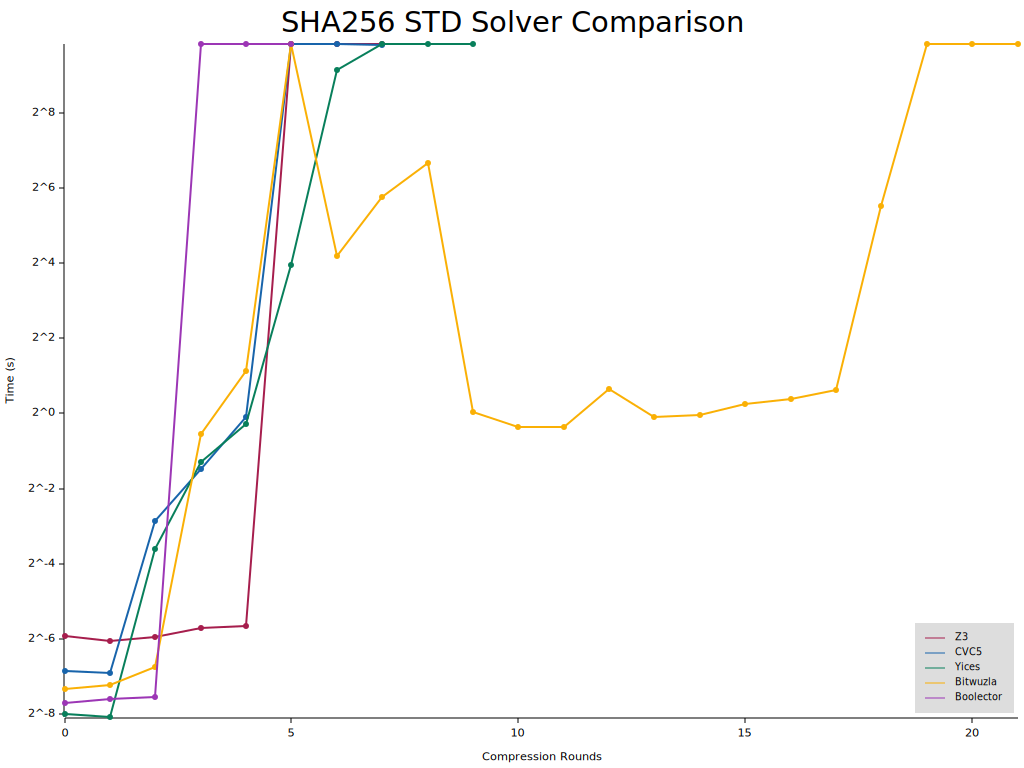
\includegraphics[width=0.7\textwidth]{../../graphs/solver_comparison_SHA256_STD.svg}
	\caption{Graph representing SHA-256 standard collisions from 1 to 20 rounds using brute-force, where each colour line represents a separate solver.
	Results ran with arguments \texttt{--round-range 1..21 --continue-on-fail true}.}
	\label{fig:sha256_std}
\end{figure}

\begin{figure}[H]
	\centering
	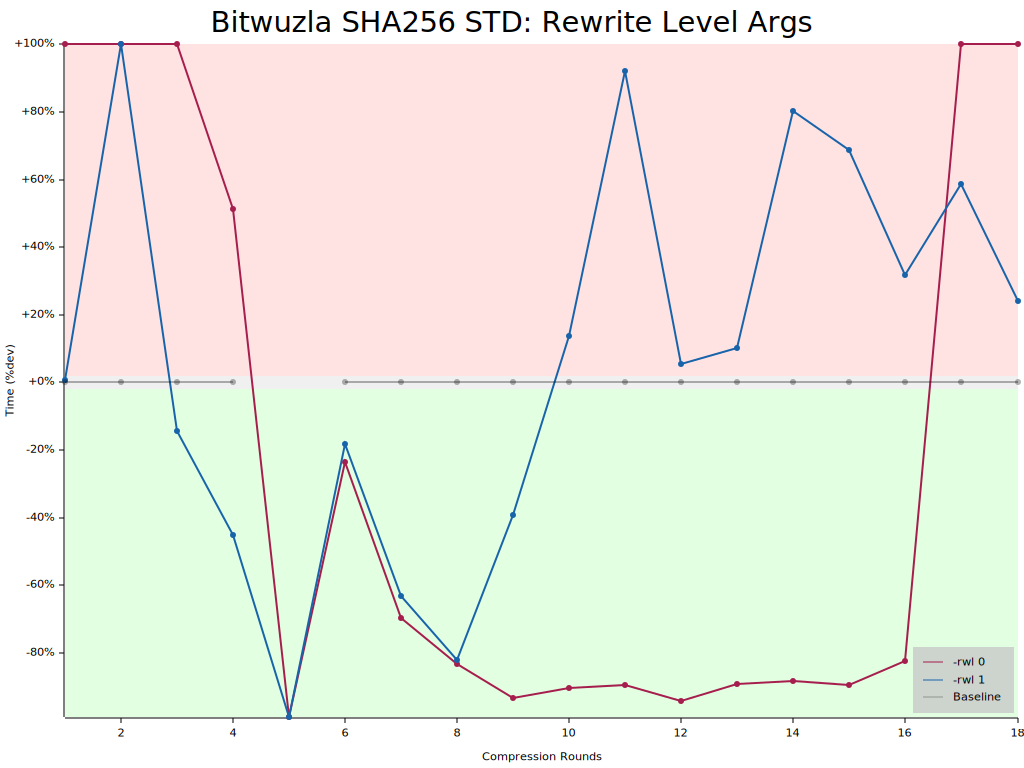
\includegraphics[width=0.7\textwidth]{../../graphs/bitwuzla_rewrite_level_args.svg}
	\caption{Bitwuzla SHA-256 standard collisions from 1 to 18 rounds using brute-force, where each colour line represents a different solver argument related to rewrite level.
	Results ran with arguments \texttt{--round range 1..19 --continue-on-fail true}}
	\label{fig:bitwuzla_rewrite}
\end{figure}

\begin{figure}[H]
	\centering
	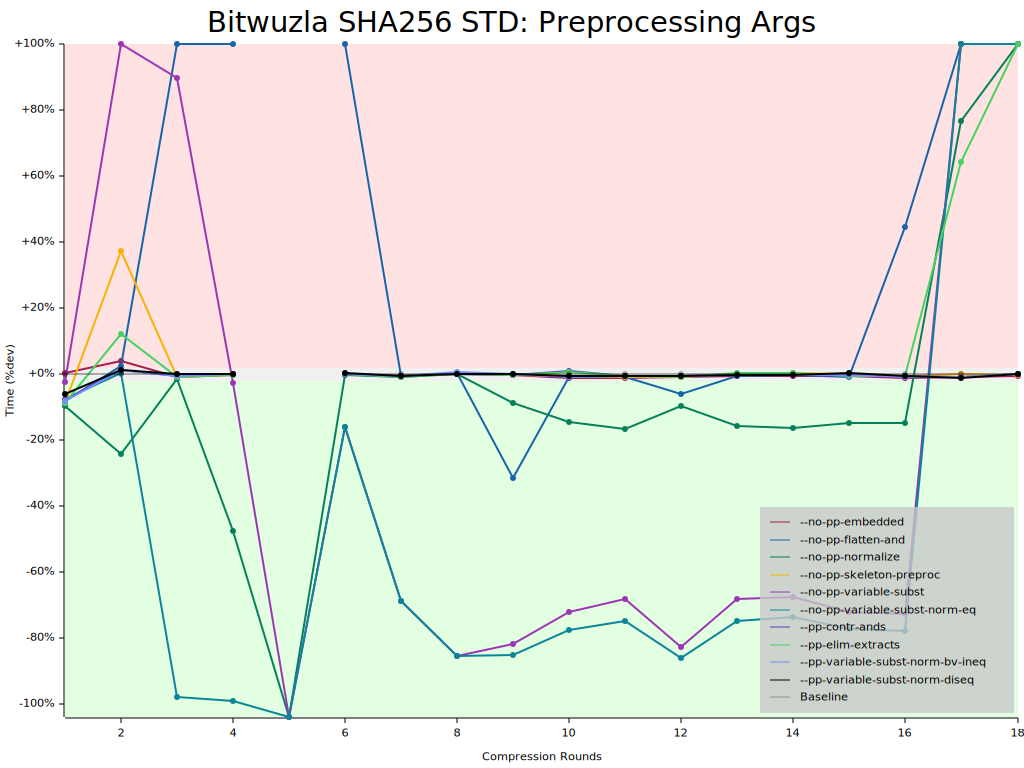
\includegraphics[width=0.7\textwidth]{../../graphs/bitwuzla_preprocessing_args.svg}
	\caption{Bitwuzla SHA-256 standard collisions from 1 to 18 rounds using brute-force, where each colour line represents a different solver argument related to preprocessing.
	Results ran with arguments \texttt{--round range 1..19 --continue-on-fail true}}
	\label{fig:bitwuzla_preprocessing}
\end{figure}

\begin{figure}[H]
	\centering
	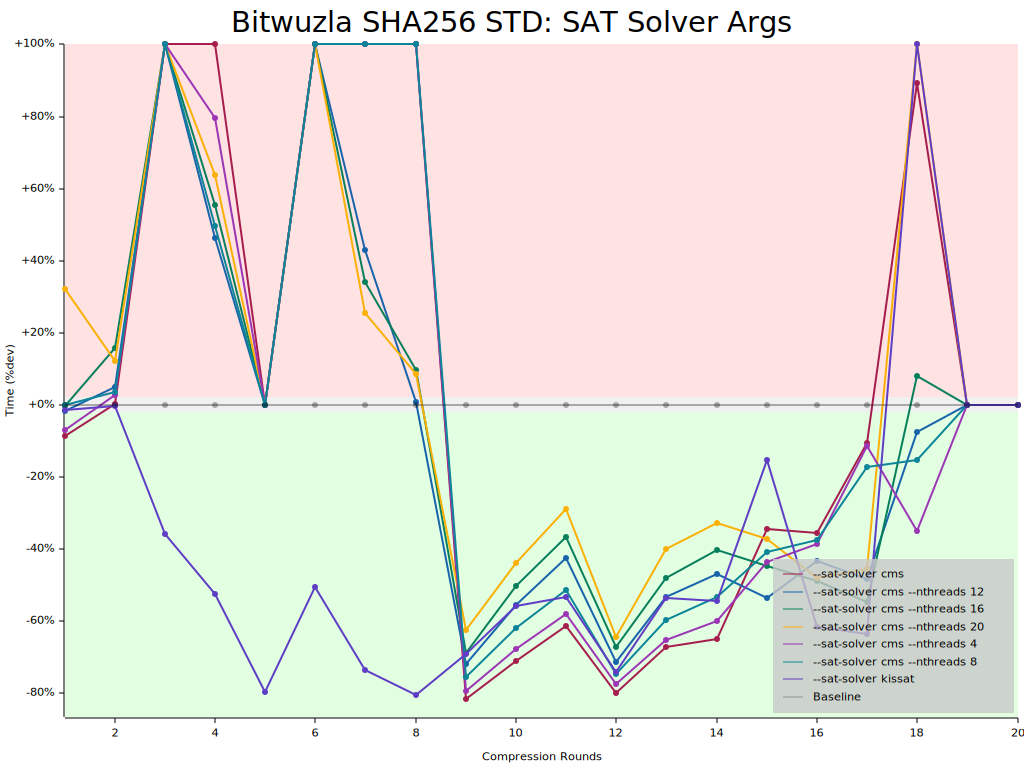
\includegraphics[width=0.8\textwidth]{../../graphs/bitwuzla_sat_solver_args.svg}
	\caption{Bitwuzla SHA-256 standard collisions from 1 to 18 rounds using brute-force, where each colour line represents a different solver argument related to the backend SAT solver.
	Results ran with arguments \texttt{--round range 1..19 --continue-on-fail true}}
	\label{fig:bitwuzla_sat_solver}
\end{figure}

\begin{figure}[H]
	\centering
	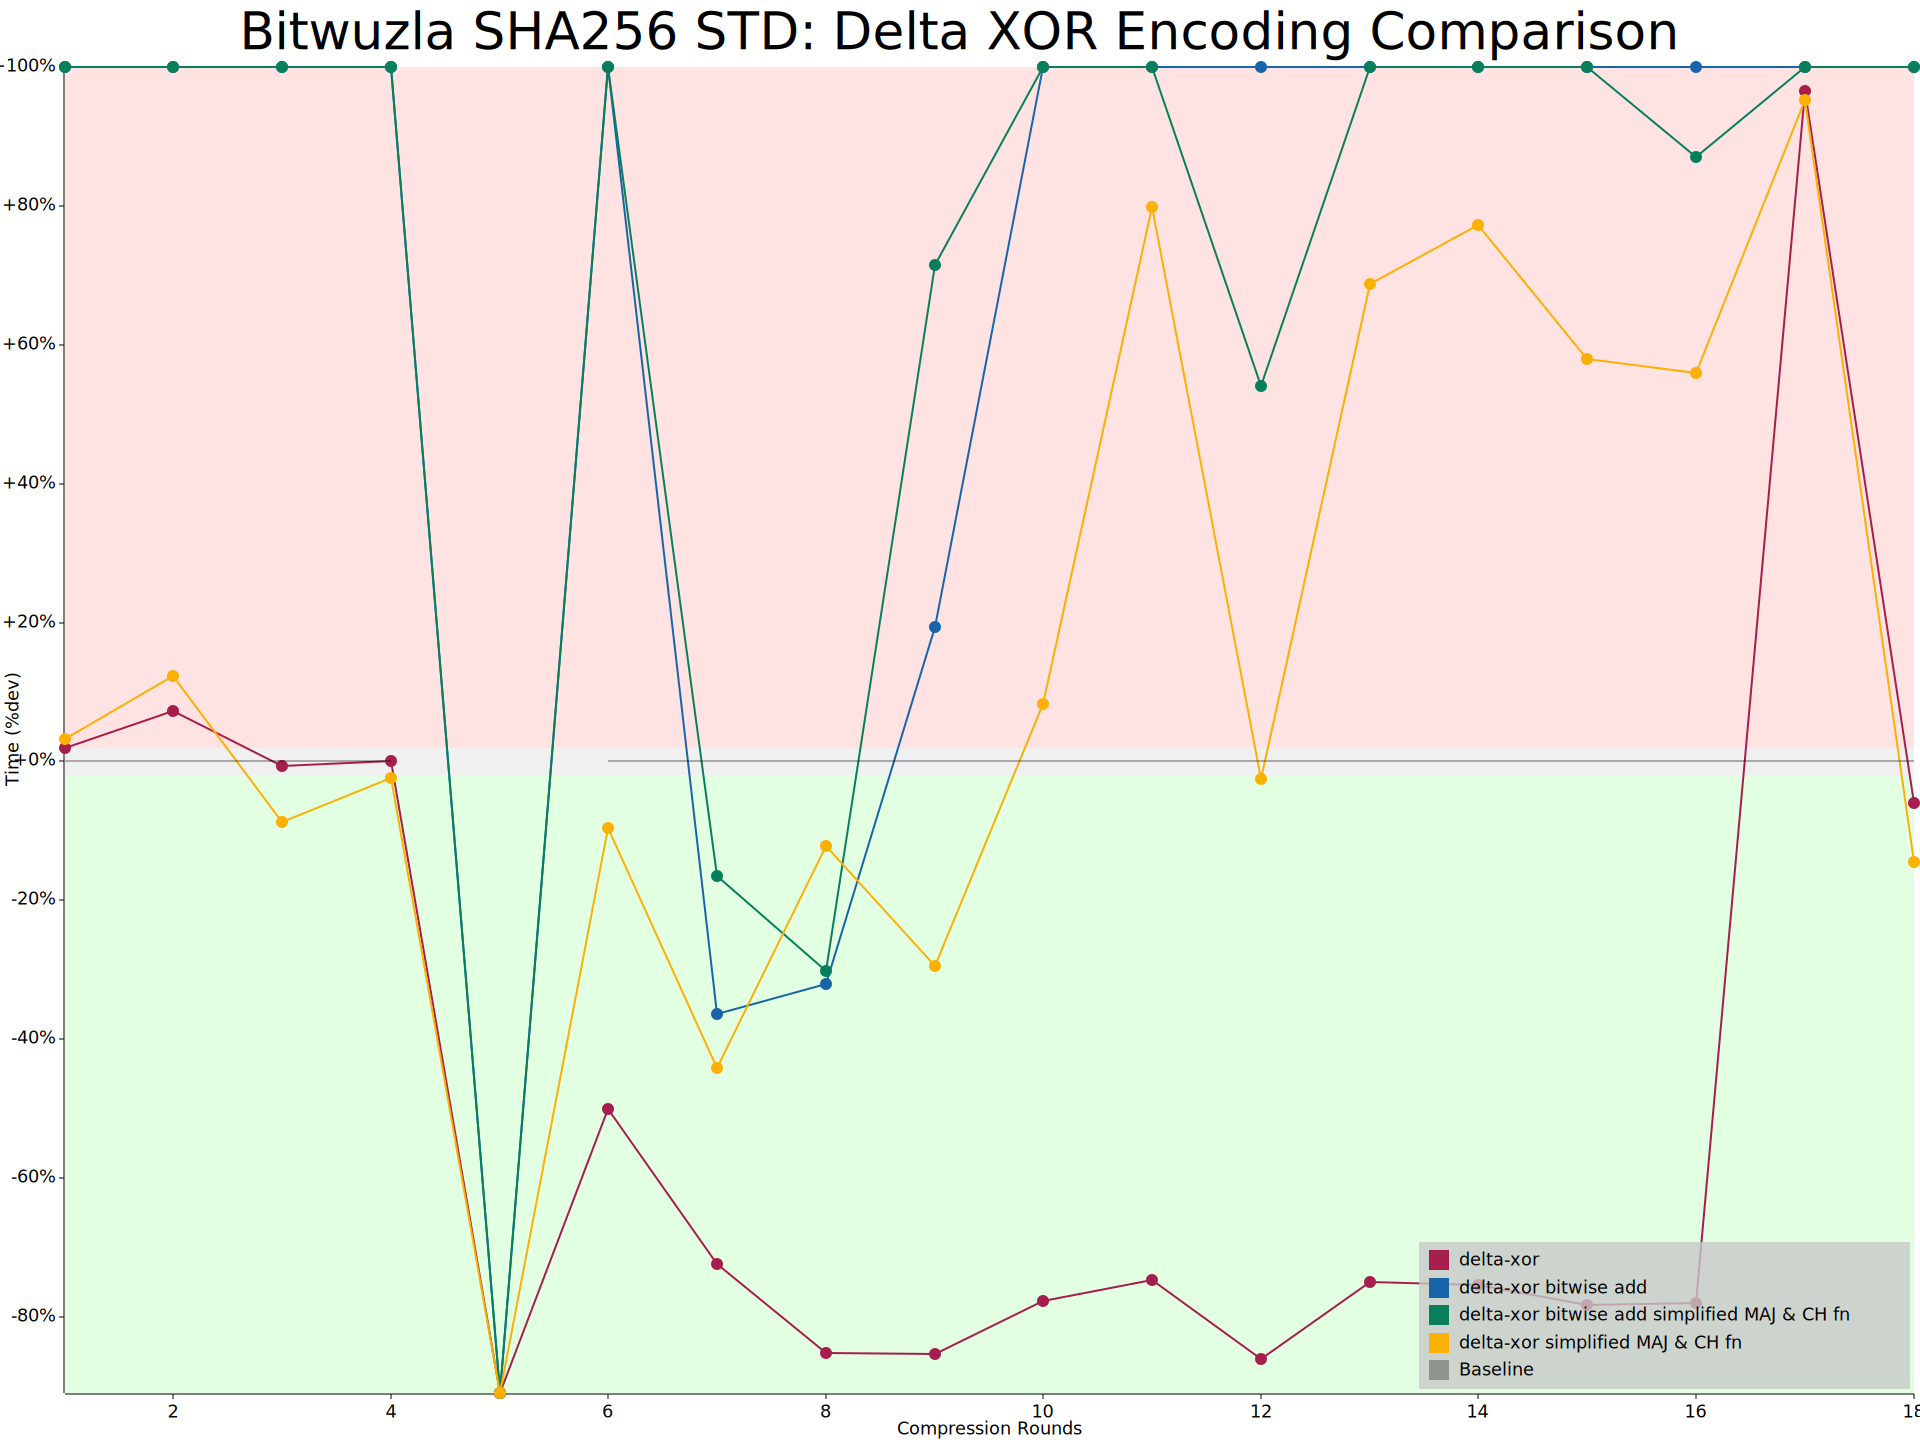
\includegraphics[width=0.8\textwidth]{../../graphs/bitwuzla_delta_xor_encoding_comparison.svg}
	\caption{Bitwuzla SHA-256 standard collision from 1 to 20 rounds using $\Delta_\oplus$ encoding. Where each colour line represents a different encoding variant.
	Results ran with arguments \texttt{--round-range 1..19 --stop-tolerance 0 --continue-on-fail true}}
	\label{fig:delta_xor}
\end{figure}

\begin{figure}[H]
	\centering
	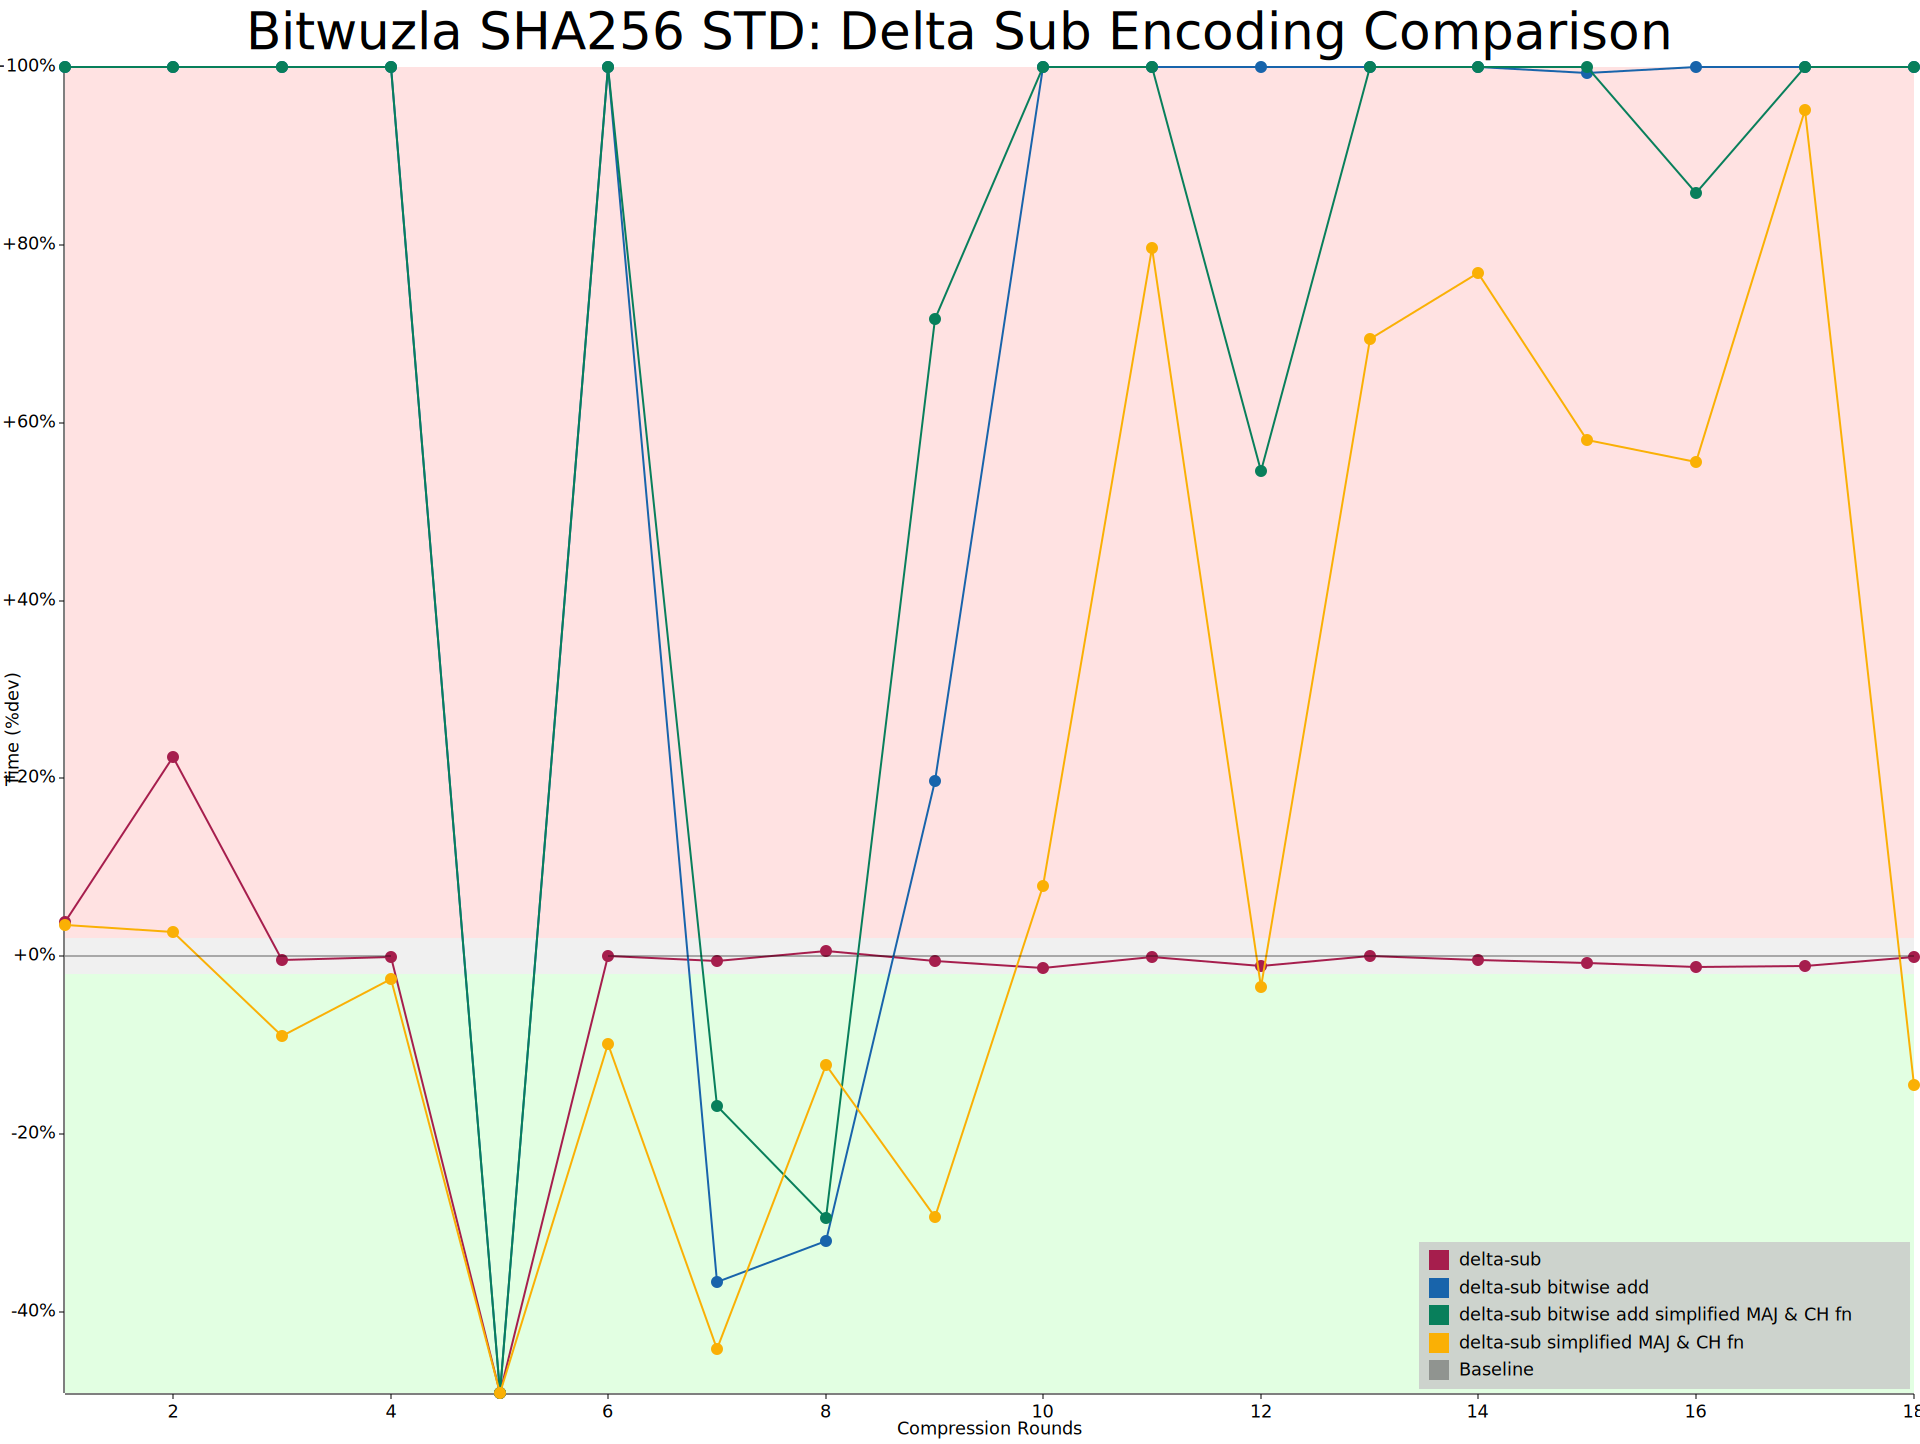
\includegraphics[width=0.8\textwidth]{../../graphs/bitwuzla_delta_sub_encoding_comparison.svg}
	\caption{Bitwuzla SHA-256 standard collision from 1 to 20 rounds using $\Delta_-$ encoding. Where each colour line represents a different encoding variant.
	Results ran with arguments \texttt{--round-range 1..19 --stop-tolerance 0 --continue-on-fail true}}
	\label{fig:delta_sub}
\end{figure}

\pagebreak
\begin{landscape}
\subsection{Significant Console Output}
Both of these outputs showcase the differential graphs with notation as \cite{li_2024}.
The $\Delta$ and $_i$ notation has been escaped due to being invalid UTF-8 in LaTeX.

\begin{lstlisting}[caption={14 round collision output obtained by running
\texttt{sha2-collision benchmark --solver bitwuzla --hash-function sha256 --collision-type std --round-range 14..15 -R true -E bruteforce::true}}, label=lst:collision-output-simpl]
14 rounds; SHA256 STD collision; Bitwuzla; SMT solver PID: 57943
File: smt/SHA256_STD_14_ALTADD.smt2
CV   : 6a09e667 bb67ae85 3c6ef372 a54ff53a 510e527f 9b05688c 1f83d9ab 5be0cd19
CV'  : 6a09e667 bb67ae85 3c6ef372 a54ff53a 510e527f 9b05688c 1f83d9ab 5be0cd19
M    : ffffffff ffffffff ffffffff ffffffff ffffffff ffffffff ffffffff ffffffff ffffffff ffffffff ffffffff ffffffff ffffffff ffffffe9 00000000 00000000
M'   : 7fffffff ddf3fdbf 7c8b10a7 de0fffbf a1ec023f 9dec01bf ffffffff 7fffffff 7fffffff ffffffff ffffffff ffffffff ffffffff ffffffe9 00000000 00000000
Hash : 1121e8fd ad9d9f9f 5e16068c 8acbfb6b 9cde4233 a73a2f5f dc9ced0a d8f47aa2 (Valid? true)
Hash': 1121e8fd ad9d9f9f 5e16068c 8acbfb6b 9cde4233 a73a2f5f dc9ced0a d8f47aa2 (Valid? true)


 i |                A                 |                E                 |                W
 0 | ================================ | ================================ | u===============================
 1 | u=============================== | u=============================== | ==u===u=====uu========u==u======
 2 | ================================ | =nn==========n========u========= | u=====uu=uuu=u==uuu=uuuu=u=uu===
 3 | ================================ | u=============================== | ==u====uuuuu=============u======
 4 | ================================ | n=============================== | =u=uuuu====u==uuuuuuuu=uuu======
 5 | ================================ | u=============================== | =uu===u====u==uuuuuuuuu==u======
 6 | ================================ | ================================ | ================================
 7 | ================================ | ================================ | u===============================
 8 | ================================ | ================================ | u===============================
 9 | ================================ | ================================ | ================================
10 | ================================ | ================================ | ================================
11 | ================================ | ================================ | ================================
12 | ================================ | ================================ | ================================
13 | ================================ | ================================ | ================================
\end{lstlisting}

\pagebreak
\begin{lstlisting}[caption={14 round collision output obtained by running
\texttt{sha2-collision benchmark --solver bitwuzla --hash-function sha256 --collision-type std --round-range 14..15 -R true -E bruteforce::}}, label=lst:collision-output]
14 rounds; SHA256 STD collision; Bitwuzla; SMT solver PID: 58100
File: smt/SHA256_STD_14.smt2
CV   : 6a09e667 bb67ae85 3c6ef372 a54ff53a 510e527f 9b05688c 1f83d9ab 5be0cd19
CV'  : 6a09e667 bb67ae85 3c6ef372 a54ff53a 510e527f 9b05688c 1f83d9ab 5be0cd19
M    : 00000000 00269eb0 073a5f45 870a253d 10cf61c3 340c932a 252046ec a8e31d41 3bf4e7e6 ba76205e 9c4e594a 38c84784 c504f3aa f3ea62bc 00000000 00000000
M'   : 00900018 a97b43d8 bc209ac8 bb2001f0 a79d7d46 fe43c1a8 38304343 860d9489 7b9b7537 d7879422 20a912e5 227a74d1 6e52b216 6efc2748 00000000 00000000
Hash : 2d09ea67 bb67ae85 3c6ef372 a54ff53a 8550d704 9f05689c b00572e3 a5670f5a (Valid? true)
Hash': 2d09ea67 bb67ae85 3c6ef372 a54ff53a 8550d704 9f05689c b00572e3 a5670f5a (Valid? true)


 i |                A                 |                E                 |                W
 0 | ================================ | ================================ | ========n==n===============nn===
 1 | ========n==n==============n=u=== | =======nu==n===============nn=== | n=n=n==n=n=nnu=nun=uuu=n=nu=n===
 2 | nu===nuu==nn=n=nnn=n=n=u=un===== | ==nuuuu==nn=u=n=n==u=nnn==nnn=== | n=nnn=uu===uu=u=nu===u=un===nu=u
 3 | u=n====nn=nu=nunnn===nnunu=n==u= | ==u=unun===u===nnu==nunuu==nnu== | ==nnnu====n=u=u===u==u==nn==uu=u
 4 | unn=nu=u==uu=u===uuu==nu=uu==n=u | ===nnn=uuu==u===n==un======un=un | n=nu=nnn=u=n==u====nnn==u====n=u
 5 | n=u=uu=nnn===n=======nn========= | ==u=n=====n=u===nn====nn==n=u=== | nn==n=n==n==uunn=n=u==u=n=====u=
 6 | u===nu=n===u==u==n===u==u==u=n== | nuun==nn=n===n=n======u===n=nnnn | ===nnu=u===n=========u=nu=u=uunn
 7 | ================================ | u=u===u===n=u===u=u=n==n=n=nnn=n | ==u=unn=uuu=nnu=n===u==unu==n===
 8 | ================================ | ====n=uunuuuu==un===nnn=n=n==n=u | =n=======uu=nunnu==n==u=uu=n===n
 9 | ================================ | =n=n===nnn===n=======nn====n==== | =nu=un=nnuuu===nn=un=n===unuuu==
10 | ================================ | u====n=n==u=nnn==n===u==u==u=n== | u=nuuu==nun==uun=u==u=nun=n=unun
11 | ================================ | ================================ | ===uu=n=u=nn==n===nn==uu=n=n=u=n
12 | ================================ | ================================ | u=n=n=nu=n=n=un==u=====uu=unun==
13 | ================================ | ================================ | u==unn=u===n=nu==u===n=nunuu=u==
\end{lstlisting}
\end{landscape}

\pagebreak
\subsection{Analysis}
\label{sssec:analysis}

Figure \ref{fig:sha256_std} helps answer \ref{rq1} and showcases interesting aspects of SMT solver choice.
The first eight rounds are UNSAT, meaning no collisions exist.
As mentioned in \ref{sssec:sat-theory}, this could be due to how the IV combined with rotational working variables work.

Bitwuzla was the most consistent SMT solver, being the only one capable of finding a collision for 7 and 8 rounds.
This suggests that Bitwuzla likely has stronger reasoning capabilities for UNSAT cores as opposed to its competitors.

As most solvers struggled with higher-round collisions, Bitwuzla and MathSAT were capable of pushing through and delivering 18 and 17 rounds respectively.
Bitwuzla is the definitive winner, being both more consistent and able to deliver the most rounds within the timeout period.
This means Bitwuzla is the baseline SMT solver to beat.

Measuring Bitwuzla's brute-force capabilities, with a 12 hour timeout, no collision was found for 19 rounds. \ref{sec:full-results}

\subsubsection{Arguments}
\label{sssec:sat-solver-args}

To answer \ref{rq2}, I ran all arguments available on the most promising SMT solver, Bitwuzla.
Figures \ref{fig:bitwuzla_rewrite} and \ref{fig:bitwuzla_preprocessing} proved that adjusting Bitwuzla's arguments can significantly impact performance.
Despite this, the solvability of consecutive rounds was not meaningfully improved.

Setting the rewrite level to 0 or disabling \texttt{variable-subst} improved short-running collisions but hindered long-running ones.

Adjusting Bitwuzla's SAT solver backend arguments influenced performance.
The Kissat SAT solver backend outperformed the baseline (CaDiCal) in lower UNSAT rounds but struggled with higher-round collisions, as can be seen in \ref{fig:bitwuzla_sat_solver}.

Enabling \texttt{--bv-solver prop} negated all of Bitwuzla's performance gains against the competition. \ref{sec:full-results}
This is likely what gives Bitwuzla most of the edge compared to other solvers.

Enabling multithreading via CryptoMiniSat improved overall performance, though increasing threads beyond four (the lowest tested) led to diminishing returns.
As described in \ref{ssec:kernel-choice}, the runner's Linux Kernel could have impacted this.
However, more likely at scale, this is caused by practical trade-offs related to SMT parallelism and SMT solver memory characteristics.

\subsubsection{Encodings}
\label{sssec:encoding-analysis}

To answer \ref{rq3}, all combinations of implemented differential encodings, mentioned in \ref{sec:encoding}, have been benchmarked.
While there were no significant performance improvements, insights can be gathered from \ref{fig:delta_xor} and \ref{fig:delta_sub}.

The delta subtract encoding, did not allow the solver to reason more freely as expected, and performed within margin of error.
It did however influence the solvability of round 5, where previously no satisfiable result was found within the timeout period.

On the other hand, the delta XOR encoding proved to be impactful, especially in short-running collisions.
It did however see a noticeable spike after round 17, but on round 18 returned slightly below baseline brute-force run, remaining a promising solution to expand on.

As for the alternative bitwise add, it almost always performed worse.
However, some output collisions were simpler with less altered bits, implying the SMT solver has managed to reason more effectively to negate the effects of SHA-2's collision resistance.
A good example of this can be seen in \ref{lst:collision-output-simpl}, as opposed to the exact same parameters without the alternative bitwise add in \ref{lst:collision-output}.

$Maj$ and $Ch$ simplification proved to have some effect, but did not paint a clear enough picutre to make a conclusive answer.
In combination with other encodings, it could prove to be more useful.


\chapter{Conclusions and Discussion}
\section{Conclusion}
This work has quantatively assessed solving times for SHA-2 collisions using different SMT solvers, their arguments, and encodings.

The graphs, provided in \ref{sec:graphs}, undoubtedly answer \ref{rq1}: Bitwuzla \cite{bitwuzla} stands out as the most promising SMT solver among those tested.
While MathSAT \cite{MathSAT} performed closely, it fell short in terms of round solvability.

It is plausible that an alternative set of arguments could improve MathSAT's or another solver's performance, leaving \ref{rq2} partially unanswered.
However, it is conclusive that default arguments for Bitwuzla seem to be the most stable for round solvability and solving time.

As for \ref{rq3}, I have explored some basic encodings to provide insights.
Reasoning about differences by subtraction simply does not work -- it should not be attempted in any future work, since it seems like a dead end and waste of time.

For \ref{rq4}, I have provided a theoretical representation of reasoning about bits in \ref{ssec:base4-encoding}.
This approach could potentially perform well, and in combination with other encodings could be on par with \cite{li_2024}'s representation.

Using brute-force approaches proved ineffective, as expected, but performed significantly better than previous literature would imply.
As seen in \ref{tab:historical-collisions}, the magnitude of the attack for 18 rounds is nowhere near the current capabilities.
By identifying the most promising reasoning tools (\ref{rq1}) and their arguments (\ref{rq2}), I have established a starting point that future research can build upon.

As previously discussed in \ref{sec:smt-performance-claims}, \cite{bellini_2024} claim that MathSAT is always inferior to Yices2.
While it is plausible for other hash functions in combination with their categorising strategy, my experiments using SHA-2 yielded results that contradict their claim.
It might potentially hold true under specific encodings; however, the performance gap observed in my benchmarks suggests this is unlikely.
This is certainly not possible for a larger number of rounds, which was not taken into account with their methodology.
Consequently, one should not assert that MathSAT is always inferior to Yices2, since this is an eager generalisation.

As stated before in \ref{sec:smt-performance-claims}, no previous work has definitively and quantatively set out a baseline specific to finding the best tool for SHA-2 collisions -- therefore, this is a new and meaningful contribution to the current knowledge.

My theory mentioned in \ref{sssec:sat-theory} seems to hold true, I was unable to find any historical work to prove or disprove this.
An unsat result is always a worst-case scenario after running all possible combinations.
Therefore there exists no combinations where a collision is possible with the standard IV for under 8 rounds.

Additionally, throughout the project, I discovered underlying issues with Bitwuzla and the upstream distribution repository.
I submitted an issue and a pull request (respectively), as mentioned in (\ref{sssec:bitwuzla-issues}), thereby contributing to open-source during this project.

\section{Future Work}
\subsection{Encoding Based Work}
\label{ssec:future-encoding}
To build upon the findings from my research, I propose replicating encodings from \citet{li_2024} or \citet{alamgir_2024}, or a combination of both, and translating them to SMTLIB.
Running these encodings on Bitwuzla, the most promising SMT solver identified in my research,
would allow for comparing results with the SAT or SAT + CAS approaches outlined in their respective papers.
This comparison might reveal improvements due to heuristics at the SMT level.
To implement this, I suggest adding relevant encodings to the encoding section of the program and generating files for running on SMT solvers.

In addition to this, the \ref{ssec:base4-encoding} could be completed and ran in comparison to these encodings to more effectively answer \ref{rq4}.

\subsection{SMT Argument Exploration Work}
\label{ssec:future-argument}
During my research, time constraints limited me to exploring only the most promising solver, Bitwuzla.
However, it is plausible that other SMT solvers such as MathSAT could outperform Bitwuzla with the right combination of arguments.
To investigate this, future work could involve benchmarking each argument for interested solvers and comparing results to identify potential improvements over the baseline performance.
The current software can accommodate these tasks, given sufficient time.

\subsection{Hardware Based Work}
\label{ssec:future-hardware}
It is highly possible that processors with increased L3 cache, such as the AMD Ryzen 7 9800X3D \cite{AMD_R7_9800X3D}, may benefit solving performance due to reduced miss penalties.
SMT solving is very memory heavy, and the locality of memory hierarchy has a major performance impact.
Even in gaming and certain workstation workloads, larger L3 caches have shown to improve performance significantly. \cite{gamersnexus}
However, there is a trade-off between cache size and retrieval time. \cite{shanthi_nd}
To date, no research has quantatively assessed the effects of cache size or core clock speed on SAT/SMT solving time.
Therefore, potential future work could involve quantifying these effects and plotting correlations between hardware parameters and solving times.
The current software can run these benchmarks, but it may require additional fields in the Benchmark struct to differentiate hardware-level changes.

\subsection{Rust Language Improvements}
\label{ssec:rust-improvements}
As mentioned in \ref{ssec:graph-design}, Rust options for visualisation crates are very limited.
Additional contributions to open source could improve the situation by making the syntax a lot simpler.
Functionality, such as different line plot styles could be improved.

The smt crate, mentioned in \ref{sssec:smtlib-generation}, lacks trivial features like the ability to export to files.
It also has poor documentation compared to the standard of the Rust ecosystem, where everything is verbosely documented.
This is another potential area to contribute additional work to, helping shape the ecosystem of Rust and cryptography.


% Glossary
\glsaddall
\printglossaries


% References
\bibliographystyle{plainnat}
\bibliography{references}


\begin{appendices}
	\chapter{Project Definition Document}
	\label{chap:pdd}
	The below 14 PDD pages have been included using \texttt{includepdf}.
	Page numbering, TOC, styling and appendix have remained together, as in the original PDD.
	\includepdf[pages=-]{../PDD/PDD_V1.0.pdf}

	\chapter{Reuse Summary}
	No code has been directly reused.

	The codebase bundles Colibri2 and MathSAT with their respective licences, but does not statically or dynamically link to the binaries.
	Usage of these bundled binaries is optional, and the code assumes nothing exists on the host, thus making checks that an SMT solver is present on the device.
	For the sake of generating results, these bundled tools, in addition to all previously mentioned SMT solvers, have been used with their respective licences.

	The SHA-2 implementation part of my code, was written fully by me as per guidelines of \cite{NIST_SP_180_4}, and is otherwise an open widely used standard.

	Rust being a streamlined low-level embedded language, provides the basic building blocks, known as the standard (\texttt{std}) library.
	Similarly, like with other languages, Rust requires the use of other external libraries, known as "crates", to extend functionality.
	This project makes use of multiple crates to supplement functionality of the \texttt{std} Rust library.

	Unlike C or C++, Rust does not utilise header files which may be provided by libraries, and instead directly links statically these crates built externally of the project target.
	All provided code is fully written by me using these imported building blocks.

	Full information regarding licences; for all solvers (including bundled ones), as well as crates; can be found in the README.md file of the source code, accessible both on GitHub and via the submission.


	\chapter{Produced Output}
	\section{Notes}
	This report was written in TeX and compiled to PDF.
	The tables have been created using an online tool \cite{tables_generator}.

	\section{Result Graphs}
	\label{sec:full-results}
	All graph data can be found in the form of tables in \ref{sec:full-results-tables}.
	\subsection{Solver Comparison Graphs}
% SHA-224
\begin{figure}[H]
	\centering
	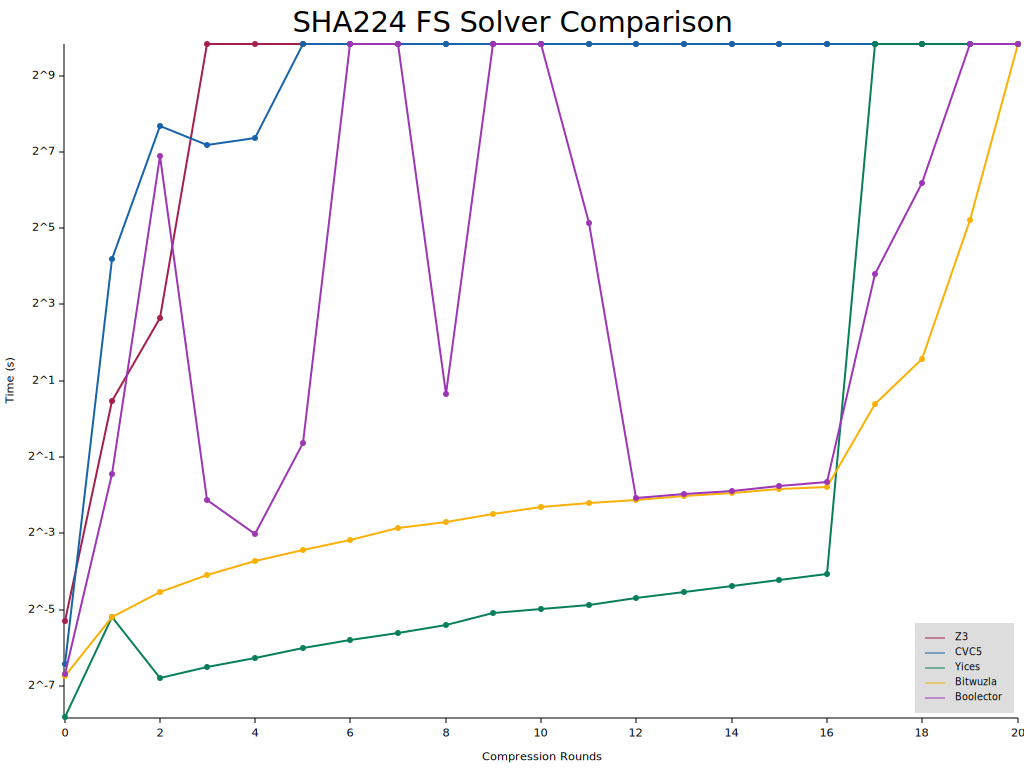
\includegraphics[width=0.8\textwidth]{../../graphs/solver_comparison_SHA224_FS.svg}
\end{figure}

\begin{figure}[H]
	\centering
	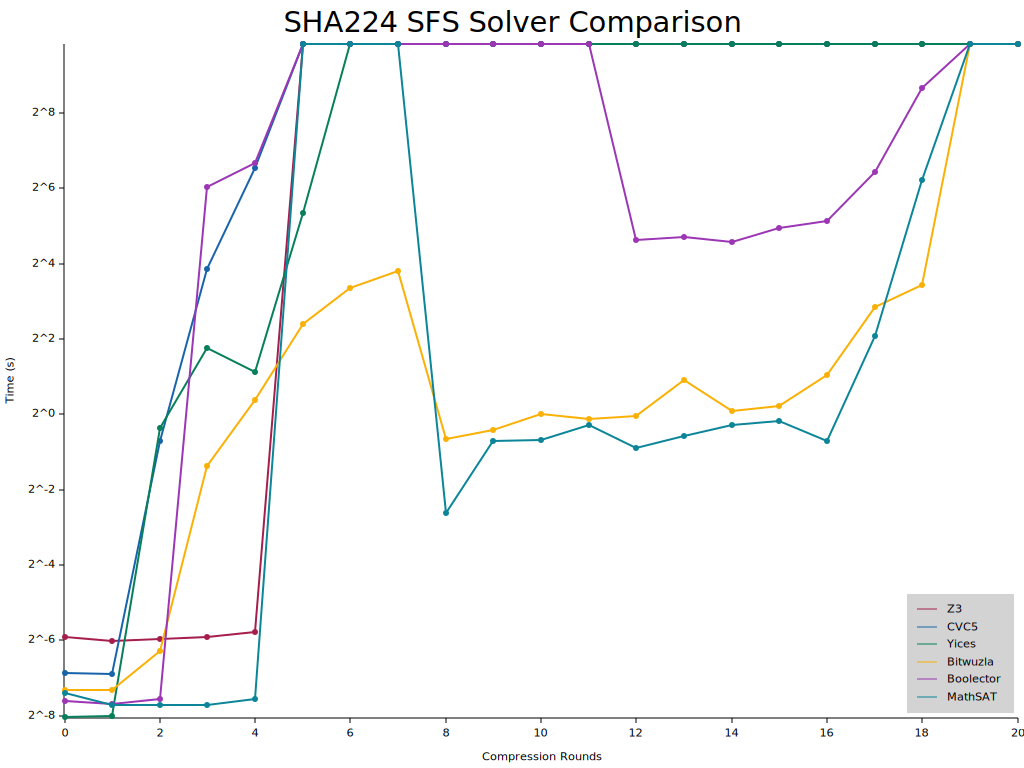
\includegraphics[width=0.8\textwidth]{../../graphs/solver_comparison_SHA224_SFS.svg}
\end{figure}

\begin{figure}[H]
	\centering
	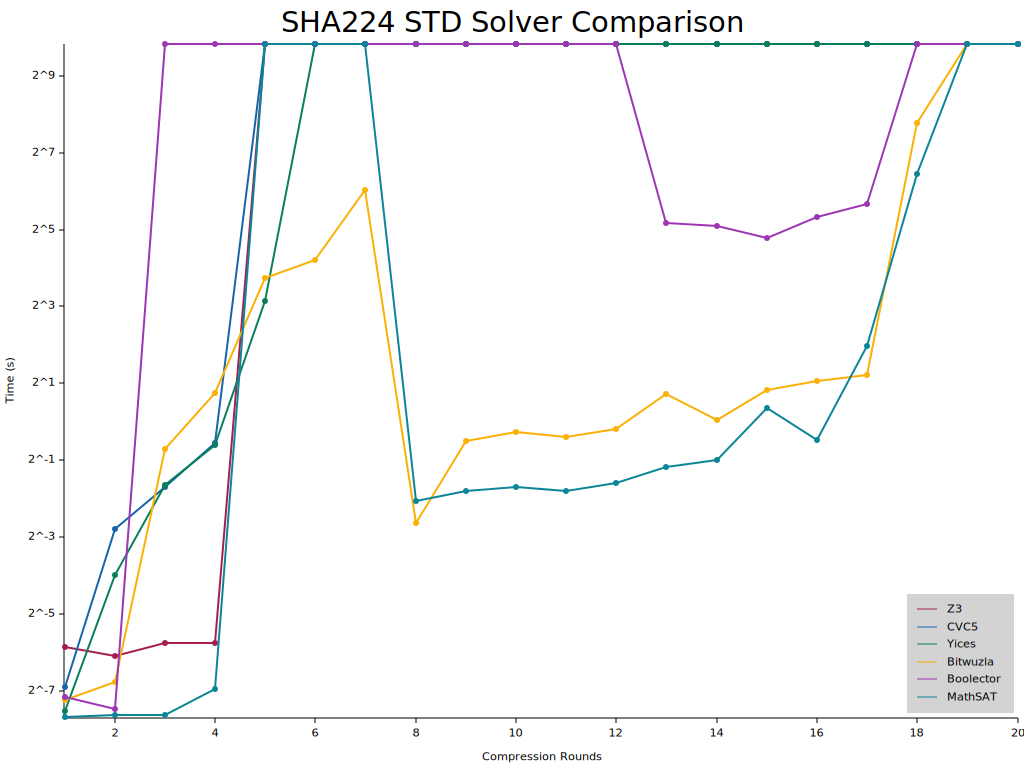
\includegraphics[width=0.8\textwidth]{../../graphs/solver_comparison_SHA224_STD.svg}
\end{figure}

% SHA-256
\begin{figure}[H]
	\centering
	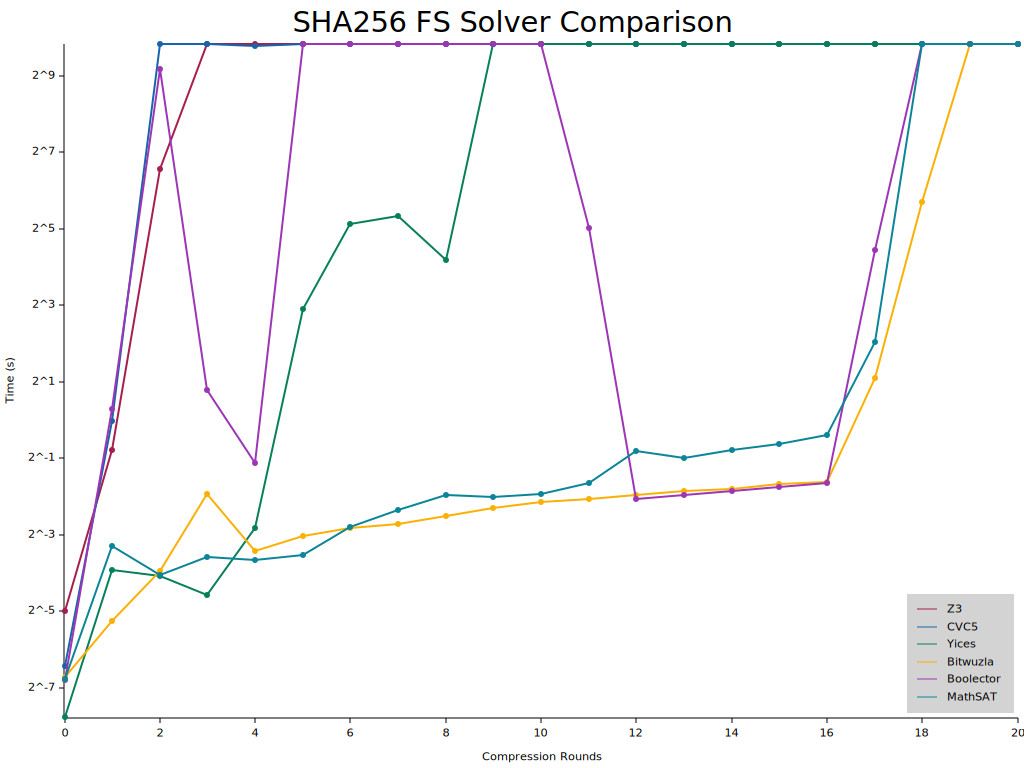
\includegraphics[width=0.8\textwidth]{../../graphs/solver_comparison_SHA256_FS.svg}
\end{figure}

\begin{figure}[H]
	\centering
	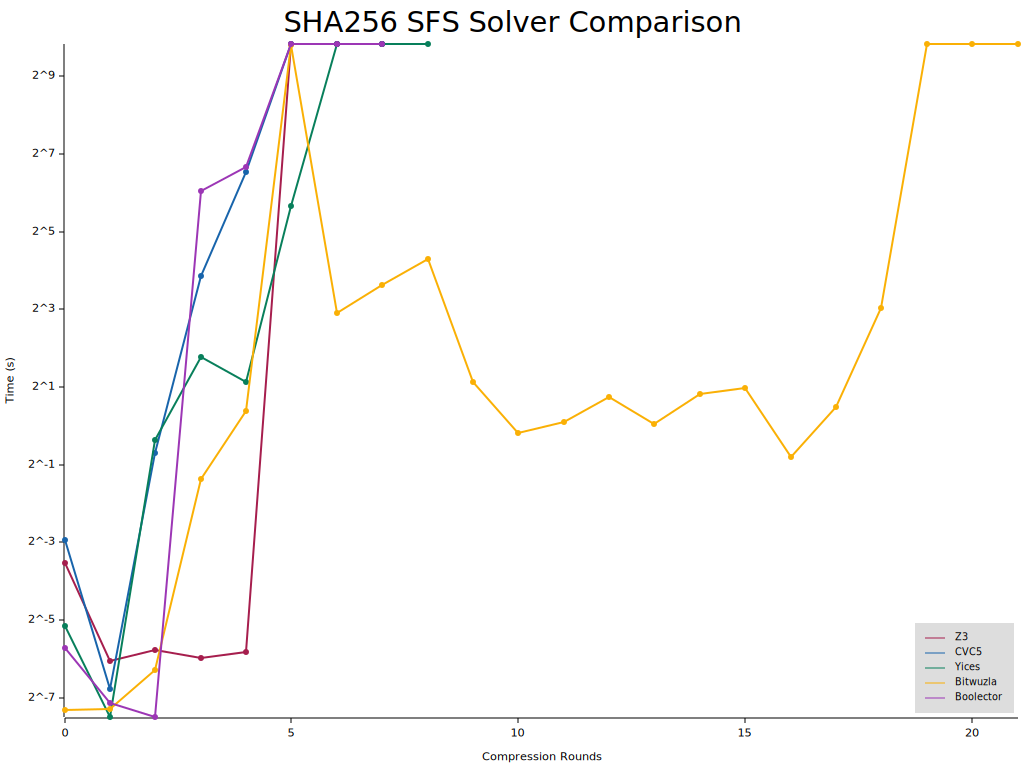
\includegraphics[width=0.8\textwidth]{../../graphs/solver_comparison_SHA256_SFS.svg}
\end{figure}

\begin{figure}[H]
	\centering
	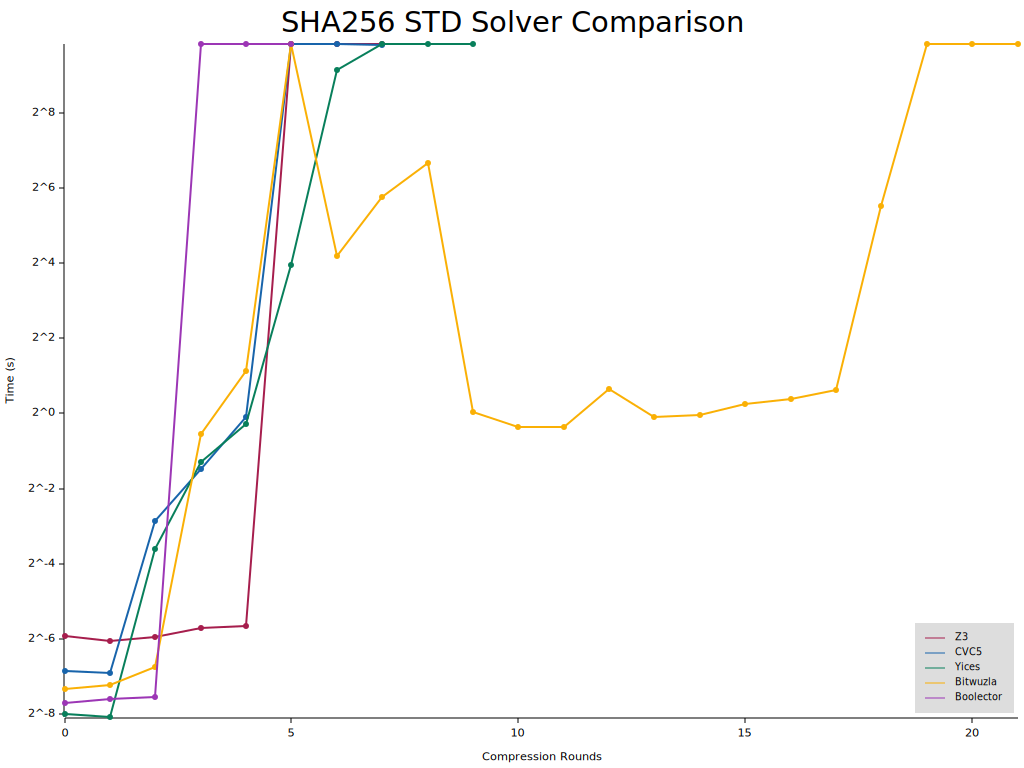
\includegraphics[width=0.8\textwidth]{../../graphs/solver_comparison_SHA256_STD.svg}
\end{figure}

% SHA-512
\begin{figure}[H]
	\centering
	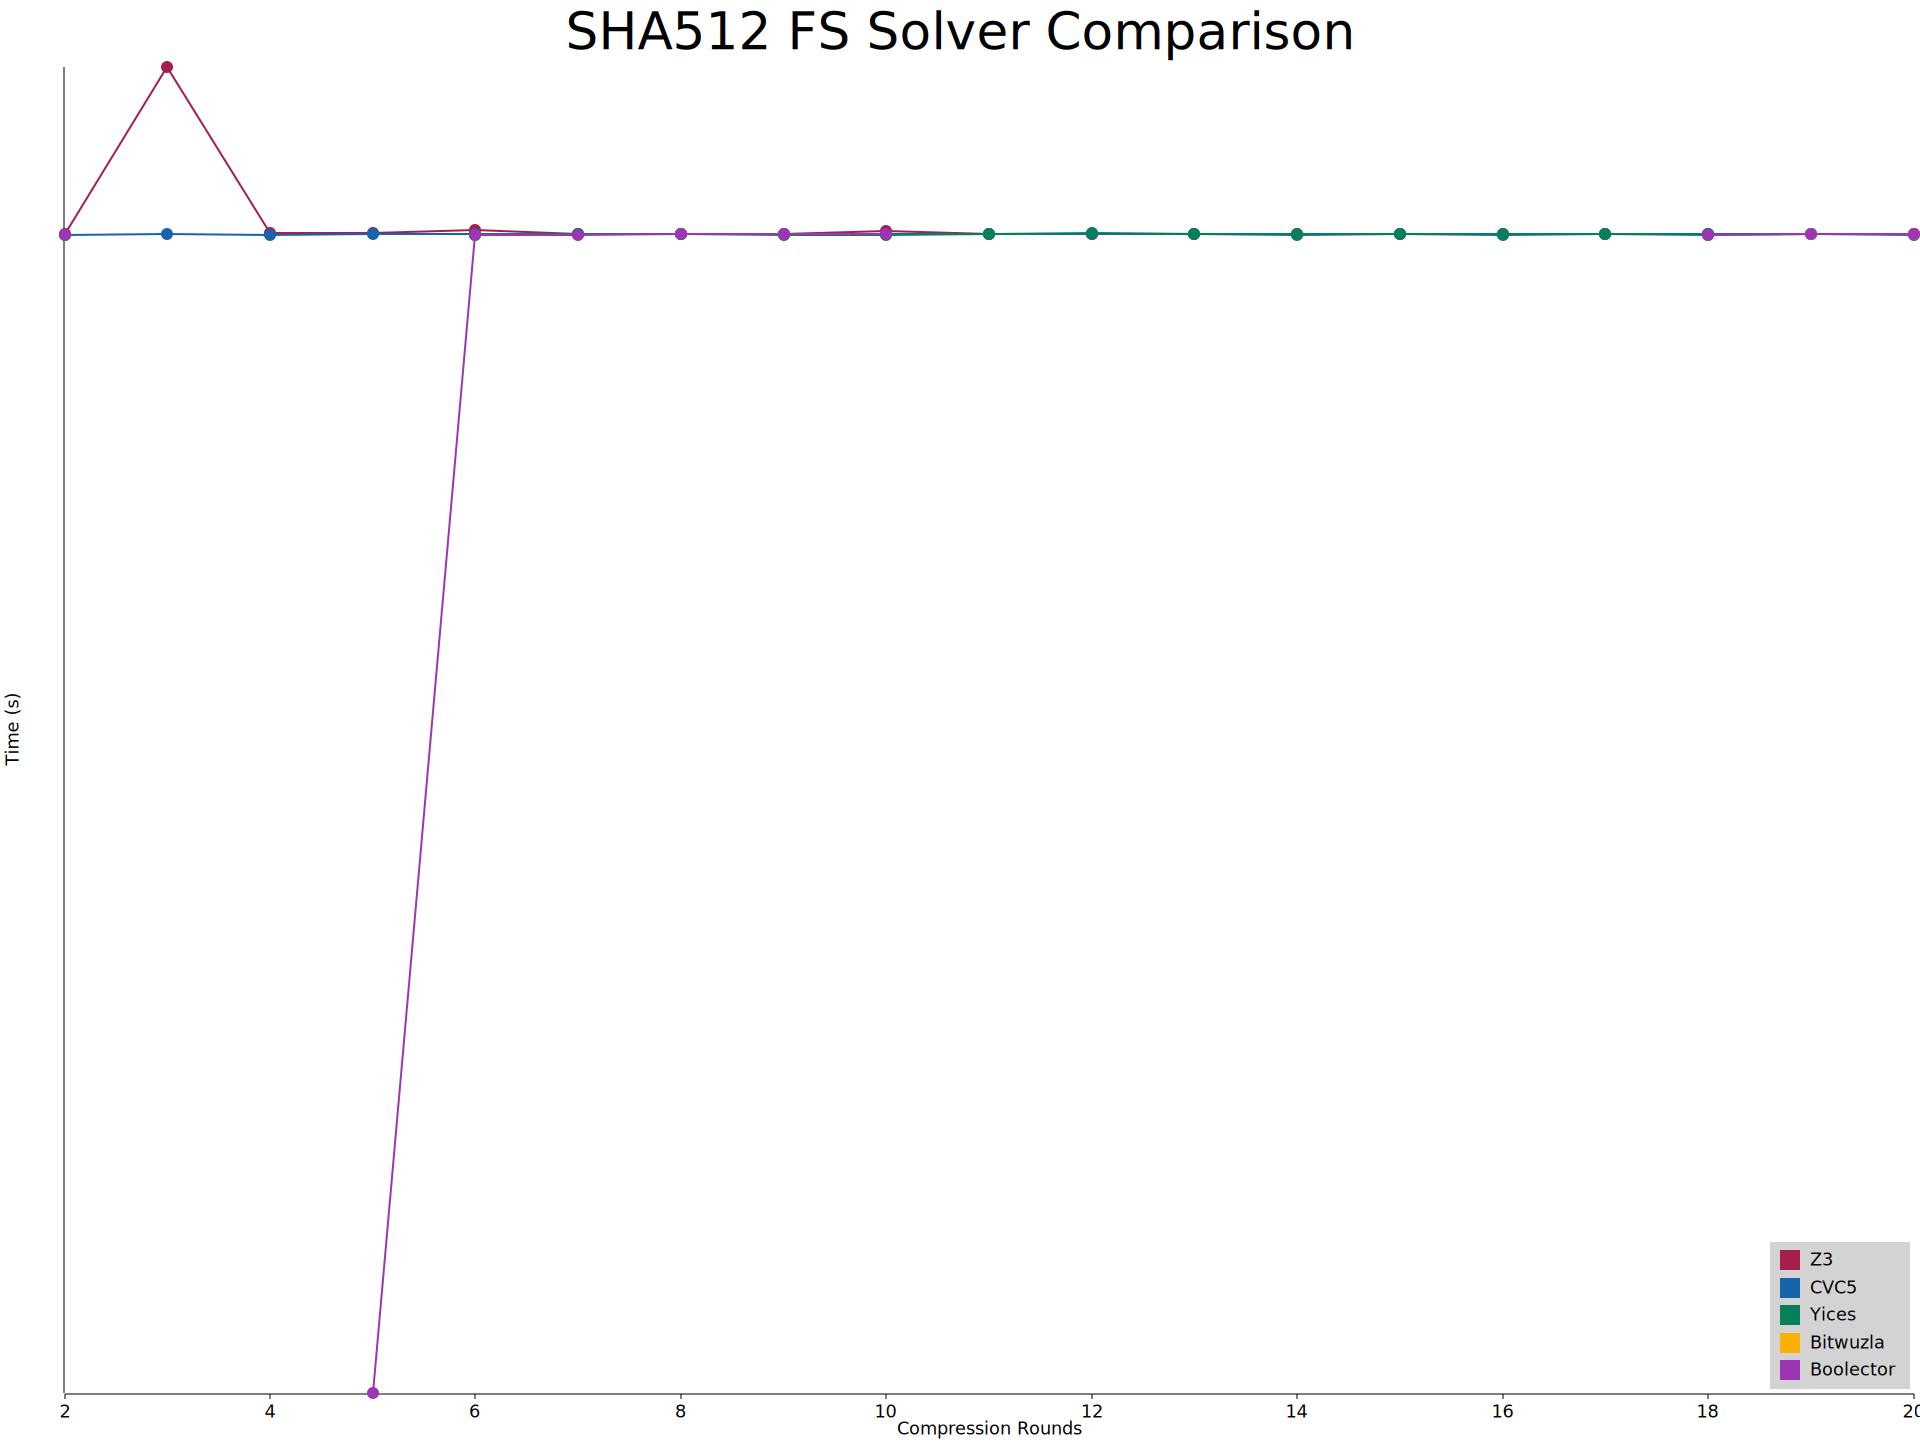
\includegraphics[width=0.8\textwidth]{../../graphs/solver_comparison_SHA512_FS.svg}
\end{figure}

\begin{figure}[H]
	\centering
	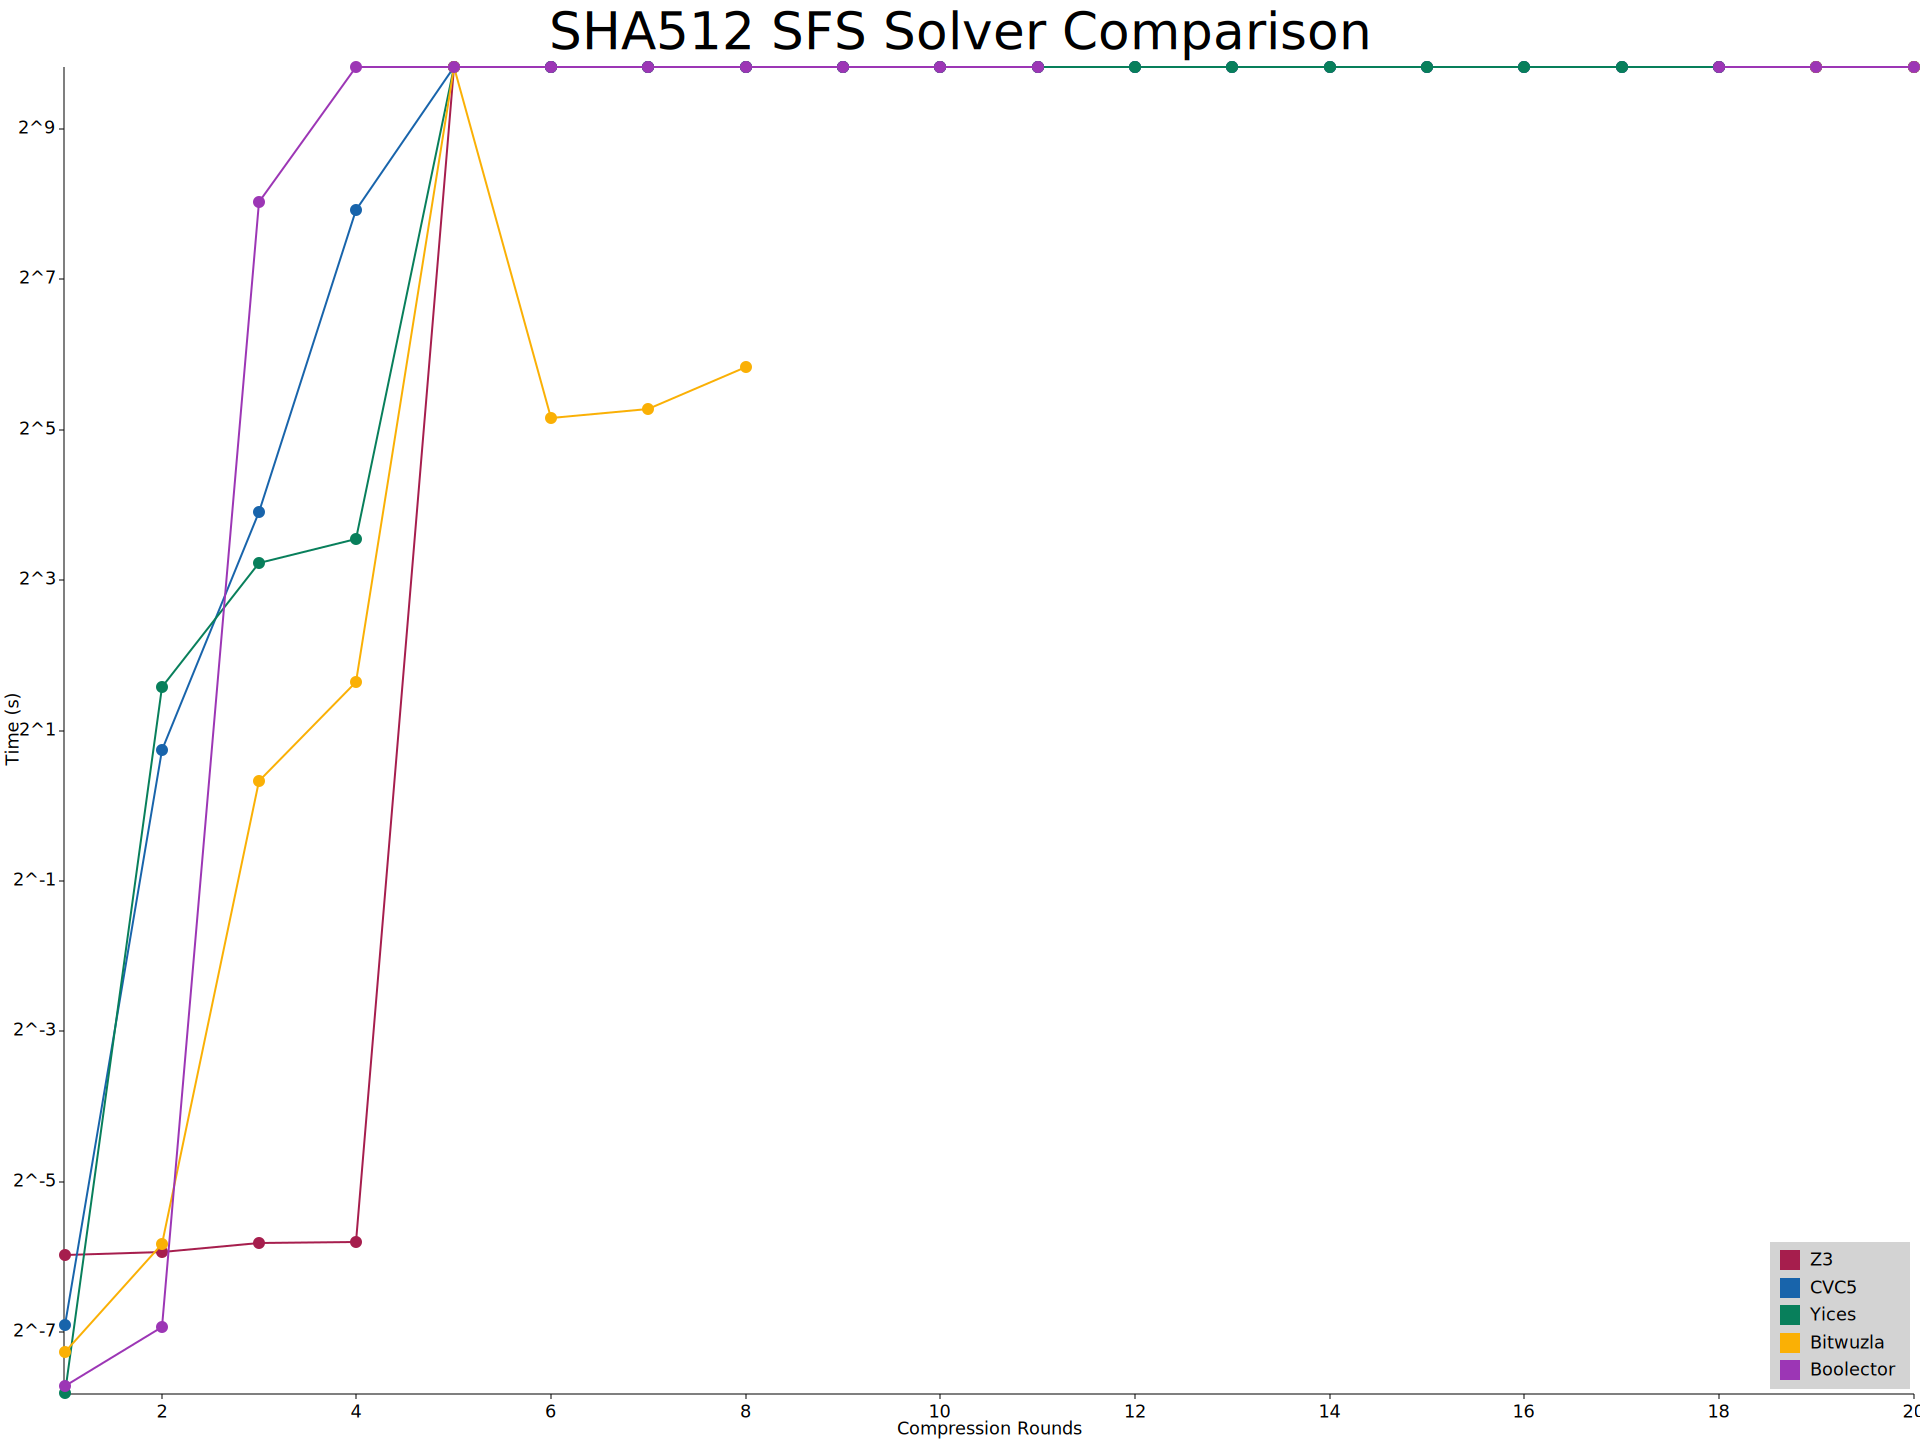
\includegraphics[width=0.8\textwidth]{../../graphs/solver_comparison_SHA512_SFS.svg}
\end{figure}

\begin{figure}[H]
	\centering
	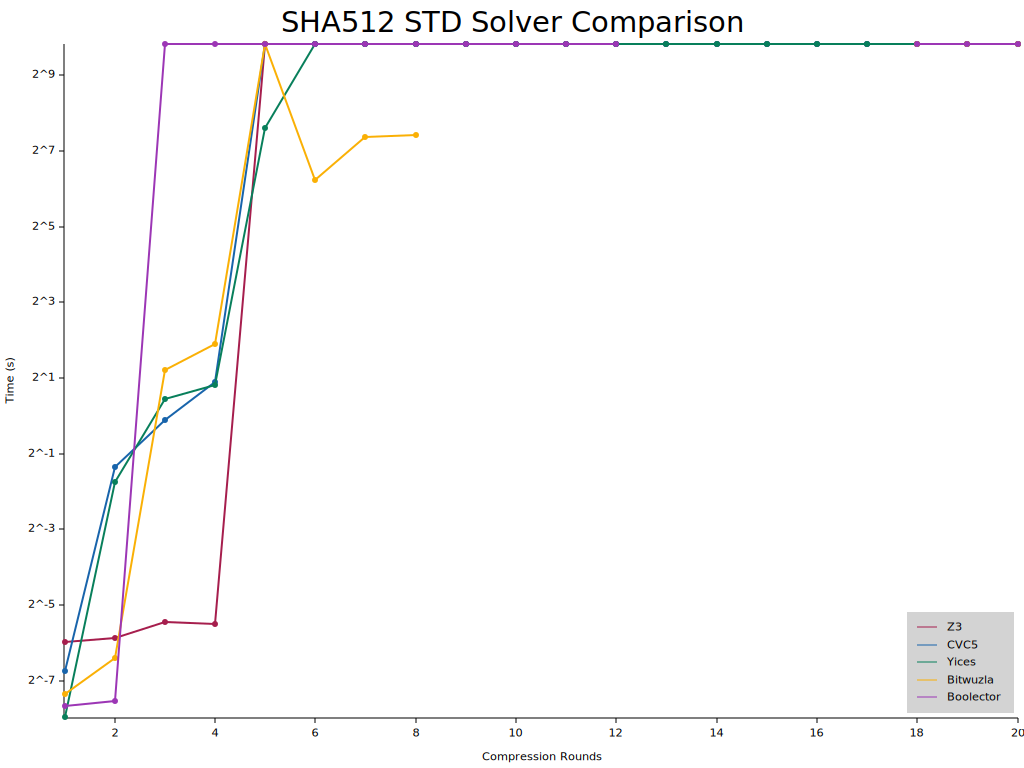
\includegraphics[width=0.8\textwidth]{../../graphs/solver_comparison_SHA512_STD.svg}
\end{figure}

\subsection{Bitwuzla Arguments}
\begin{figure}[H]
	\centering
	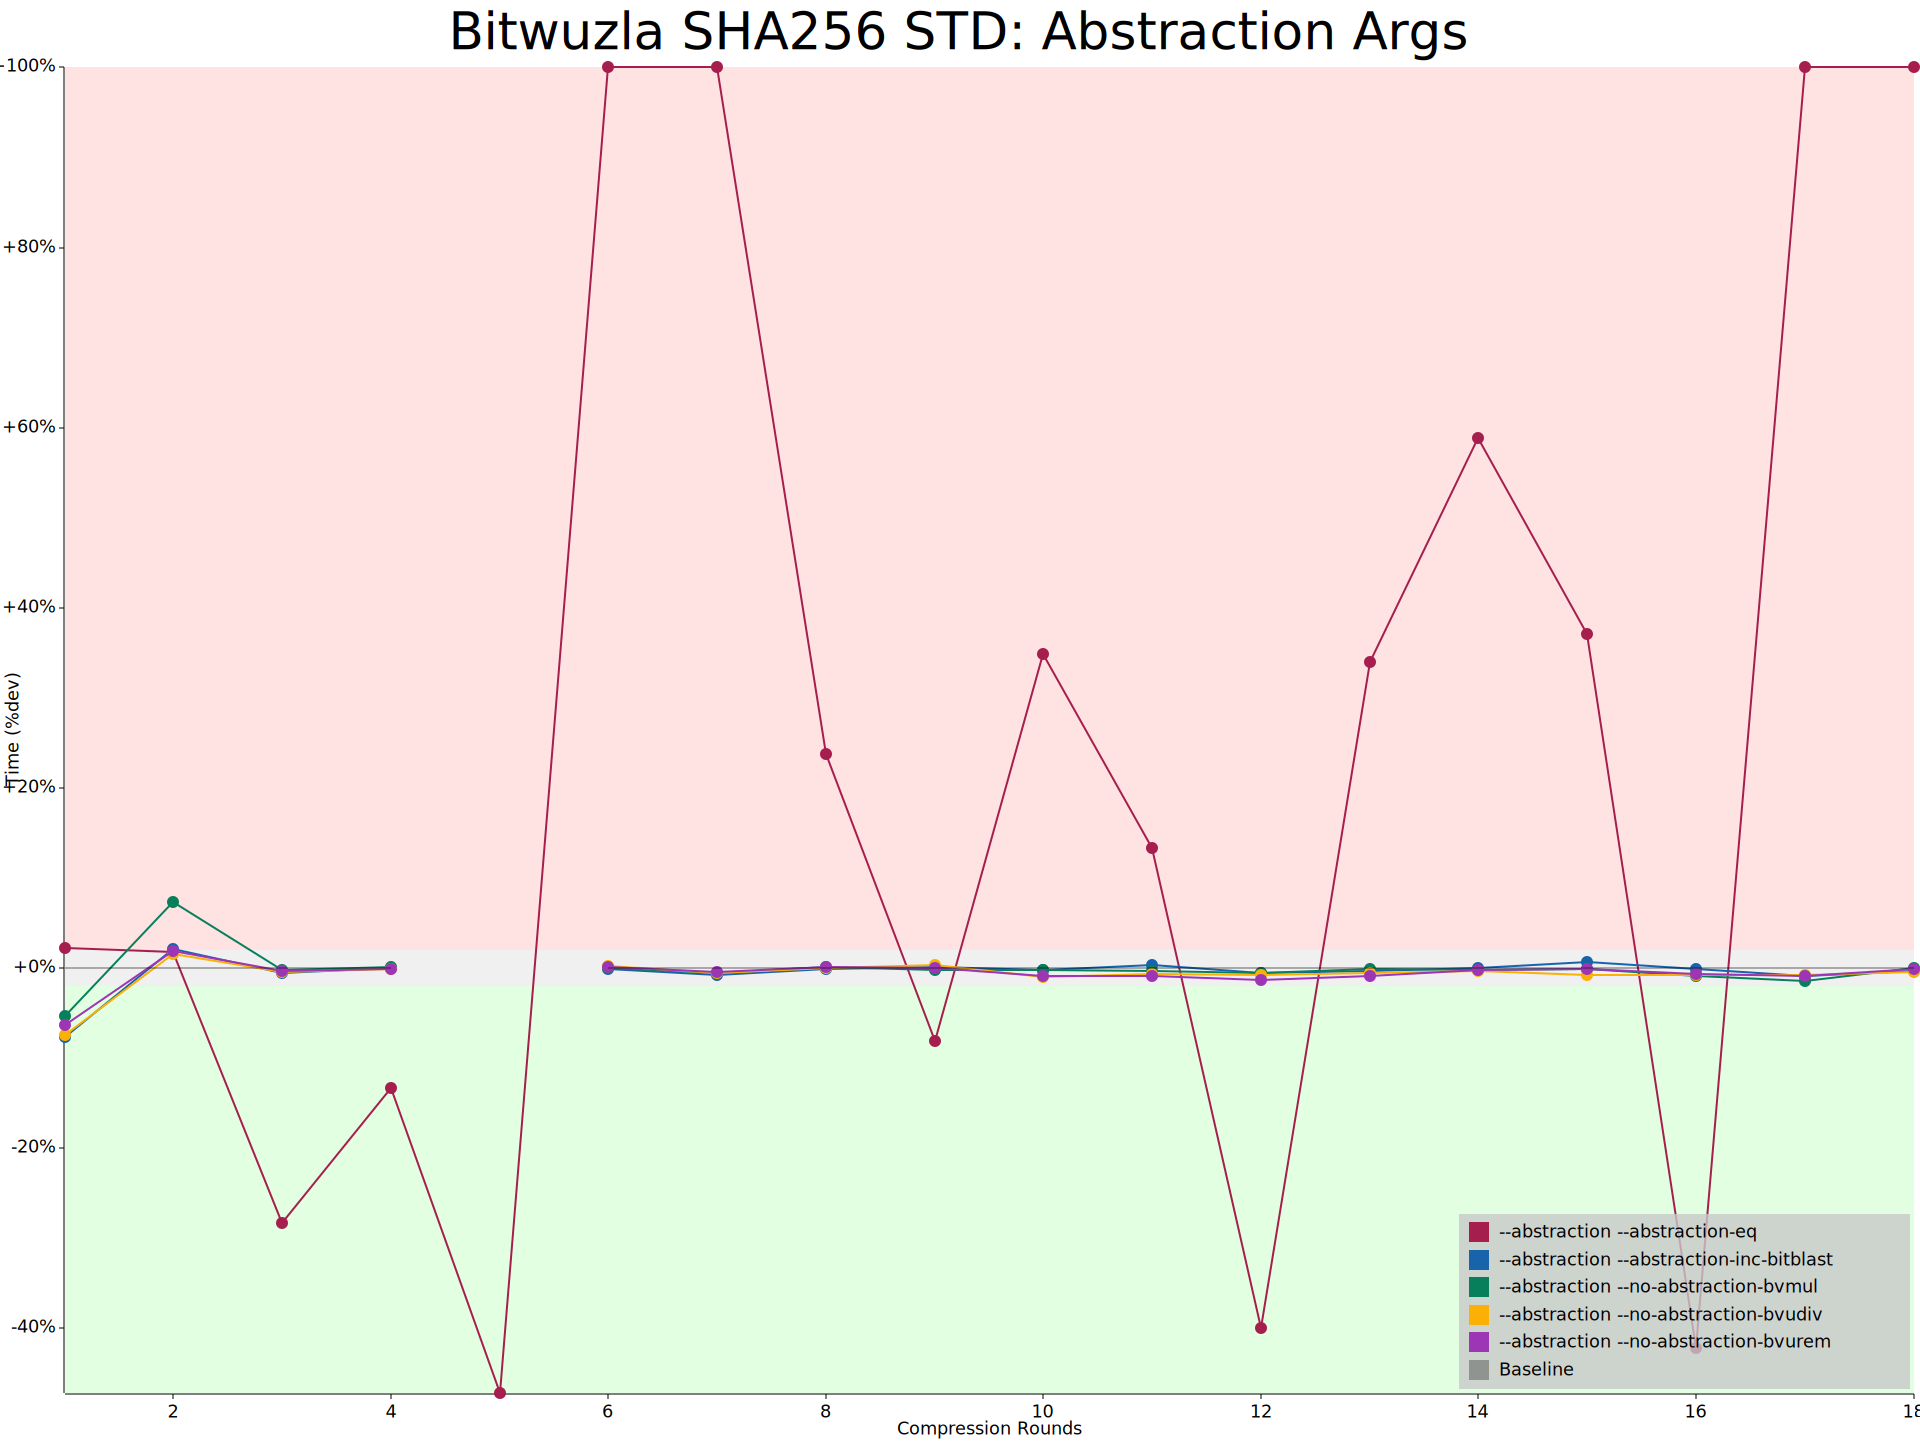
\includegraphics[width=0.8\textwidth]{../../graphs/bitwuzla_abstraction_args.svg}
\end{figure}

\begin{figure}[H]
	\centering
	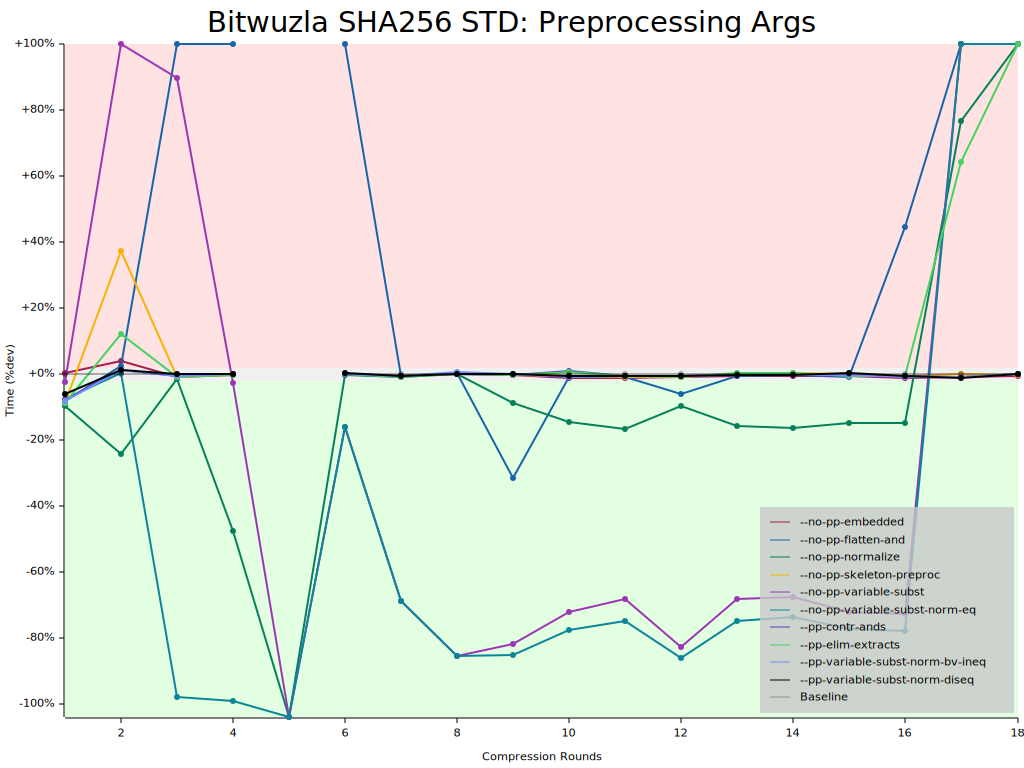
\includegraphics[width=0.8\textwidth]{../../graphs/bitwuzla_preprocessing_args.svg}
\end{figure}

\begin{figure}[H]
	\centering
	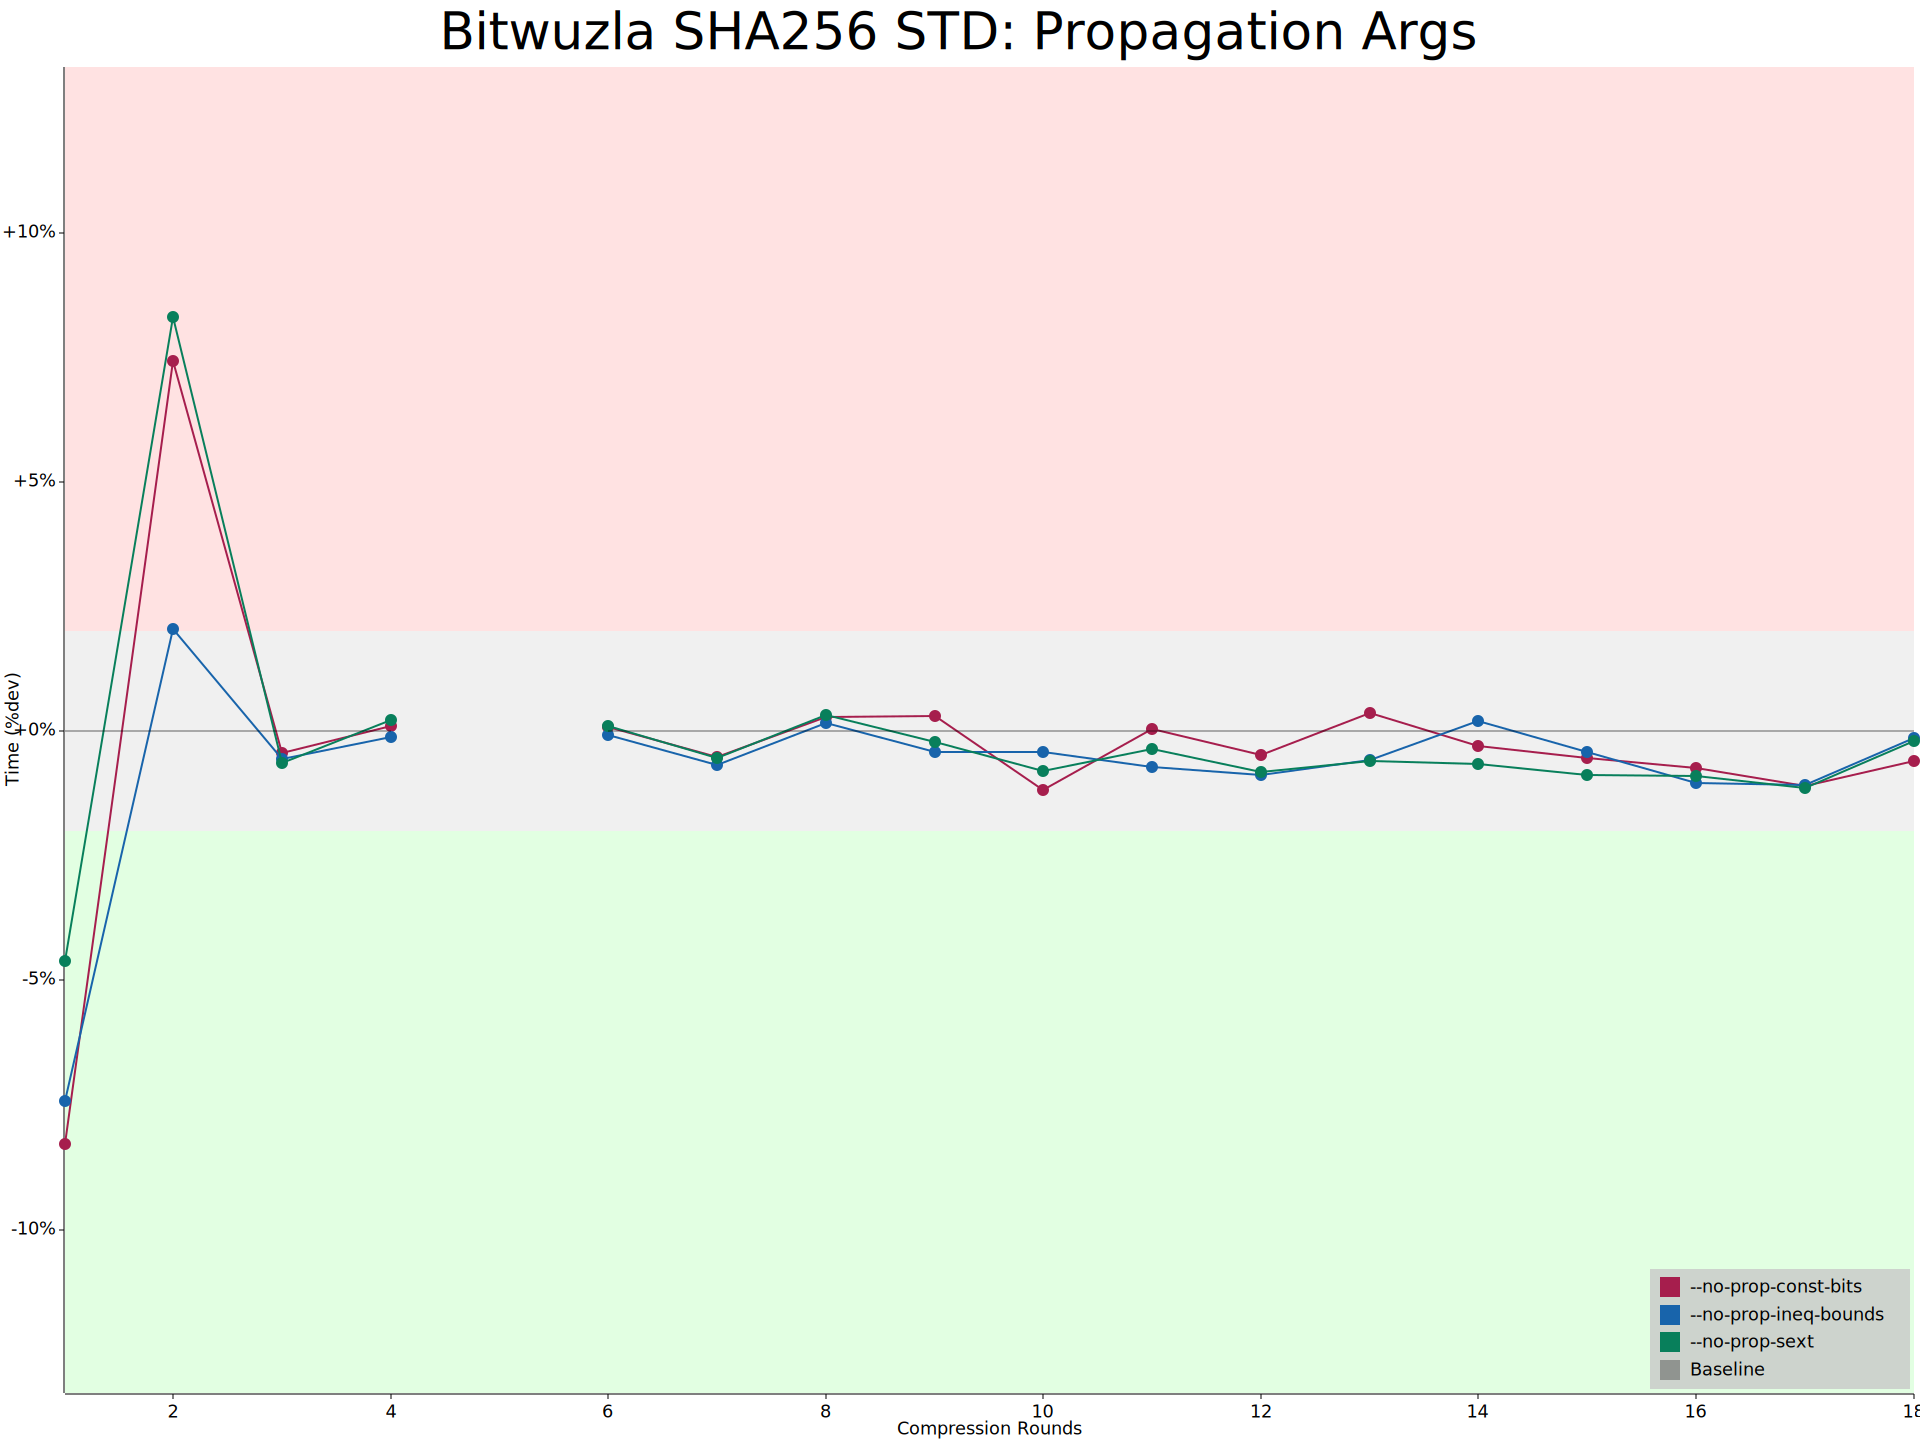
\includegraphics[width=0.8\textwidth]{../../graphs/bitwuzla_propagation_args.svg}
\end{figure}

\begin{figure}[H]
	\centering
	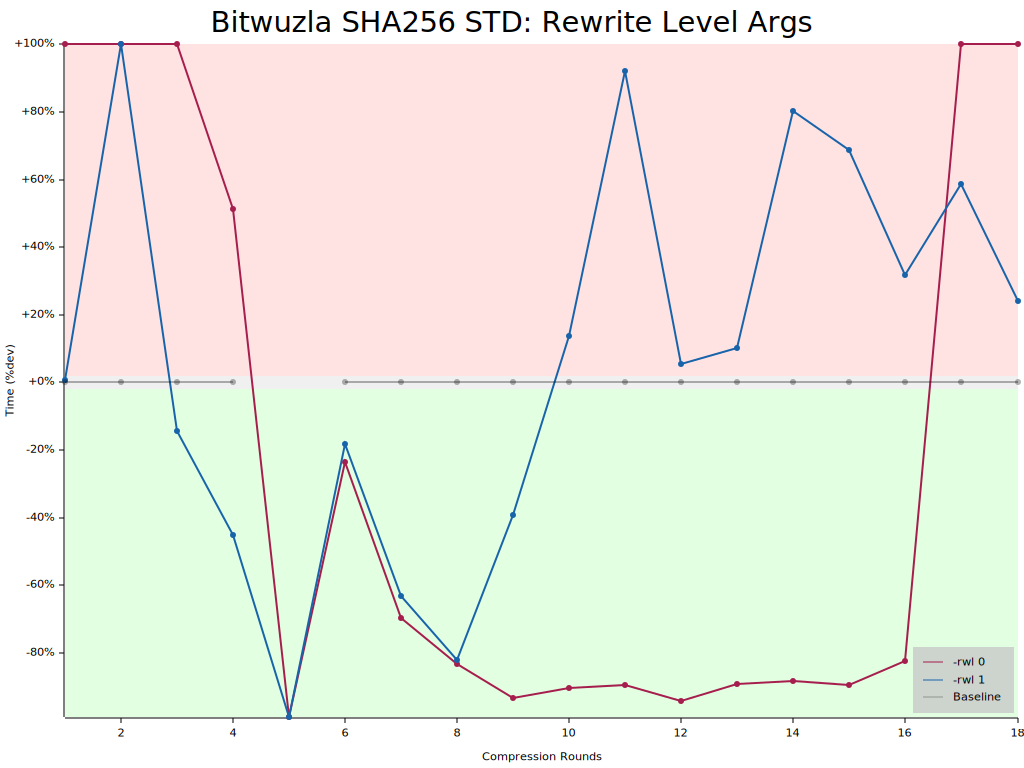
\includegraphics[width=0.8\textwidth]{../../graphs/bitwuzla_rewrite_level_args.svg}
\end{figure}

\begin{figure}[H]
	\centering
	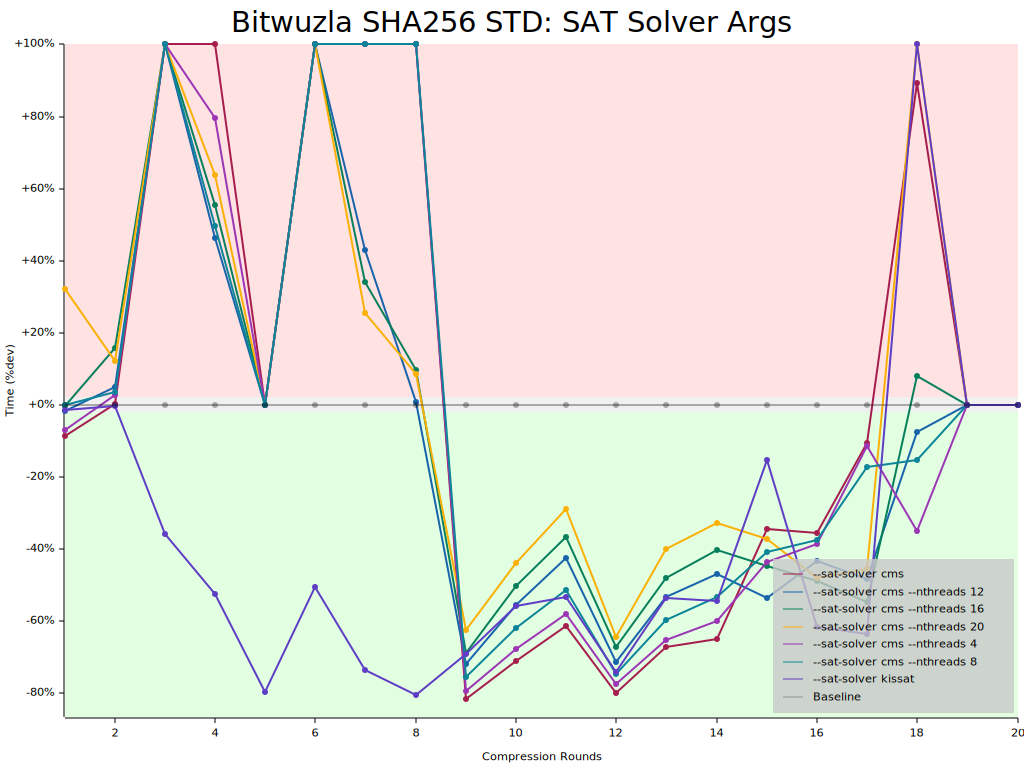
\includegraphics[width=0.8\textwidth]{../../graphs/bitwuzla_sat_solver_args.svg}
\end{figure}

\begin{figure}[H]
	\centering
	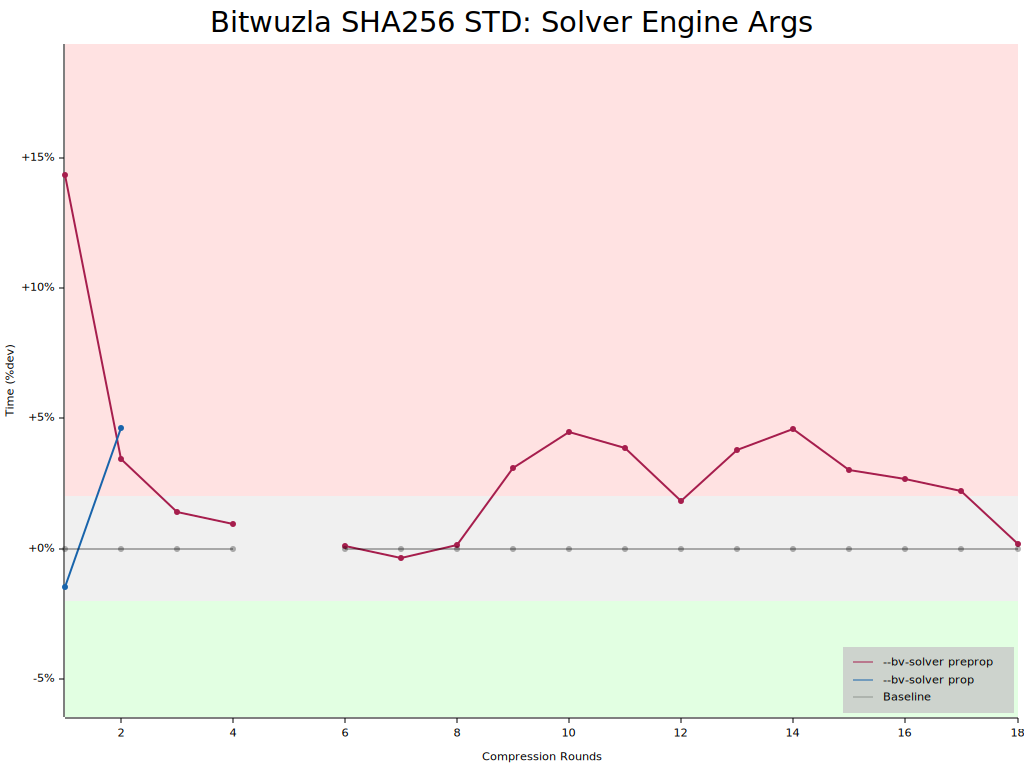
\includegraphics[width=0.8\textwidth]{../../graphs/bitwuzla_solver_engine_args.svg}
\end{figure}

\subsection{Detailed Bitwuzla Graph}

\begin{figure}[H]
	\centering
	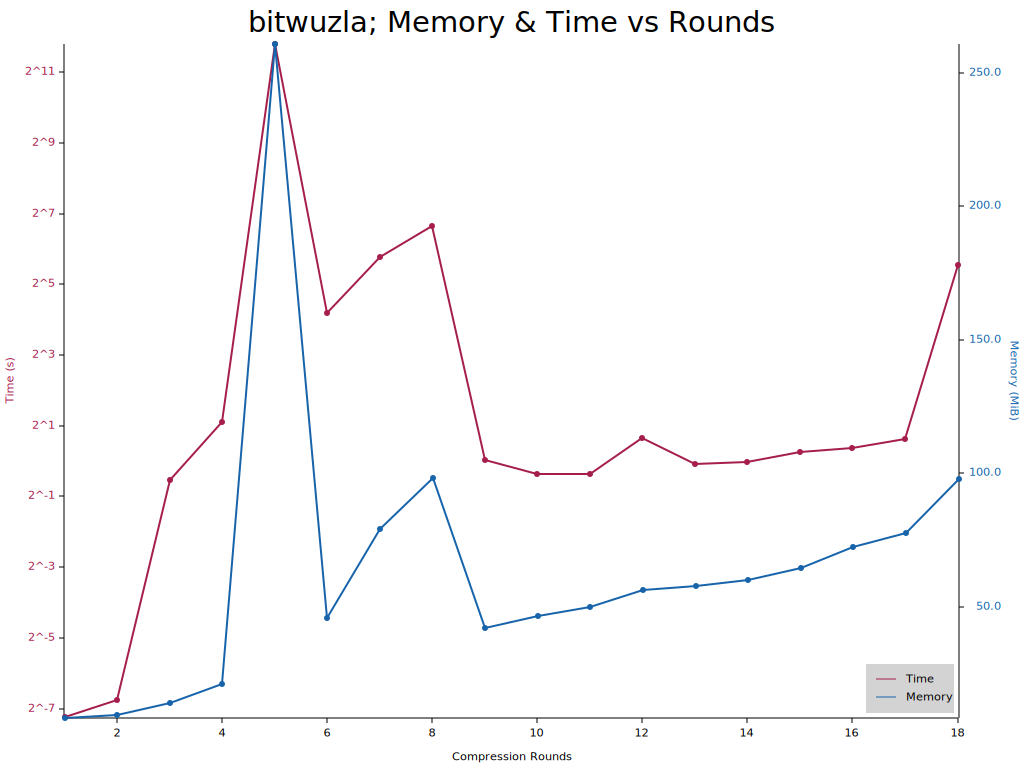
\includegraphics[width=0.8\textwidth]{../../graphs/detailed_bitwuzla_SHA256_STD.svg}
\end{figure}

\subsection{Encoding Graphs}

\begin{figure}[H]
	\centering
	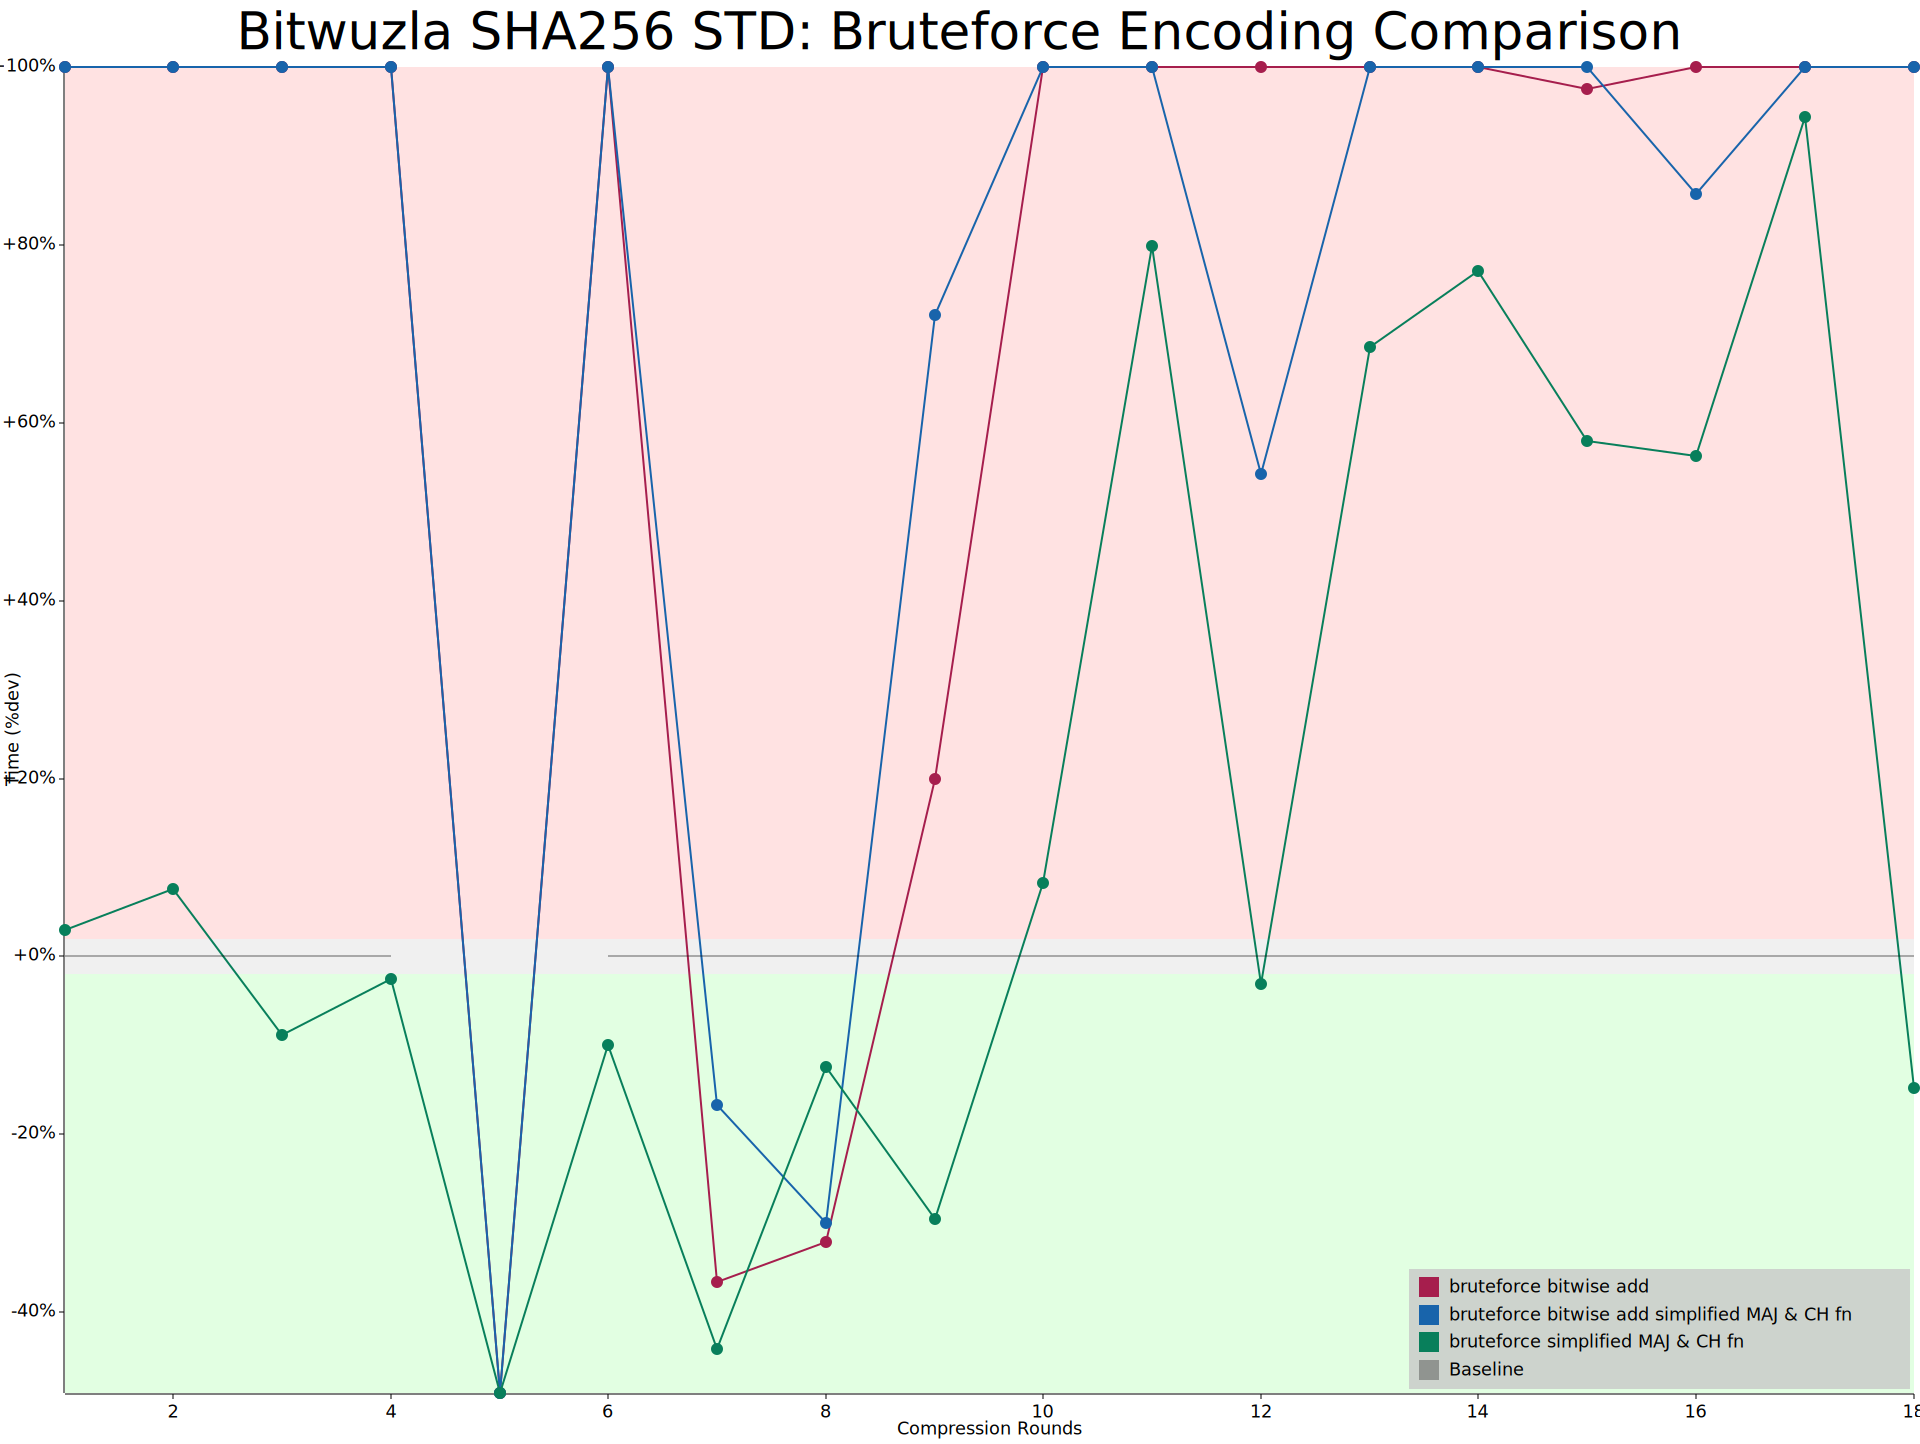
\includegraphics[width=0.8\textwidth]{../../graphs/bitwuzla_bruteforce_encoding_comparison.svg}
\end{figure}

\begin{figure}[H]
	\centering
	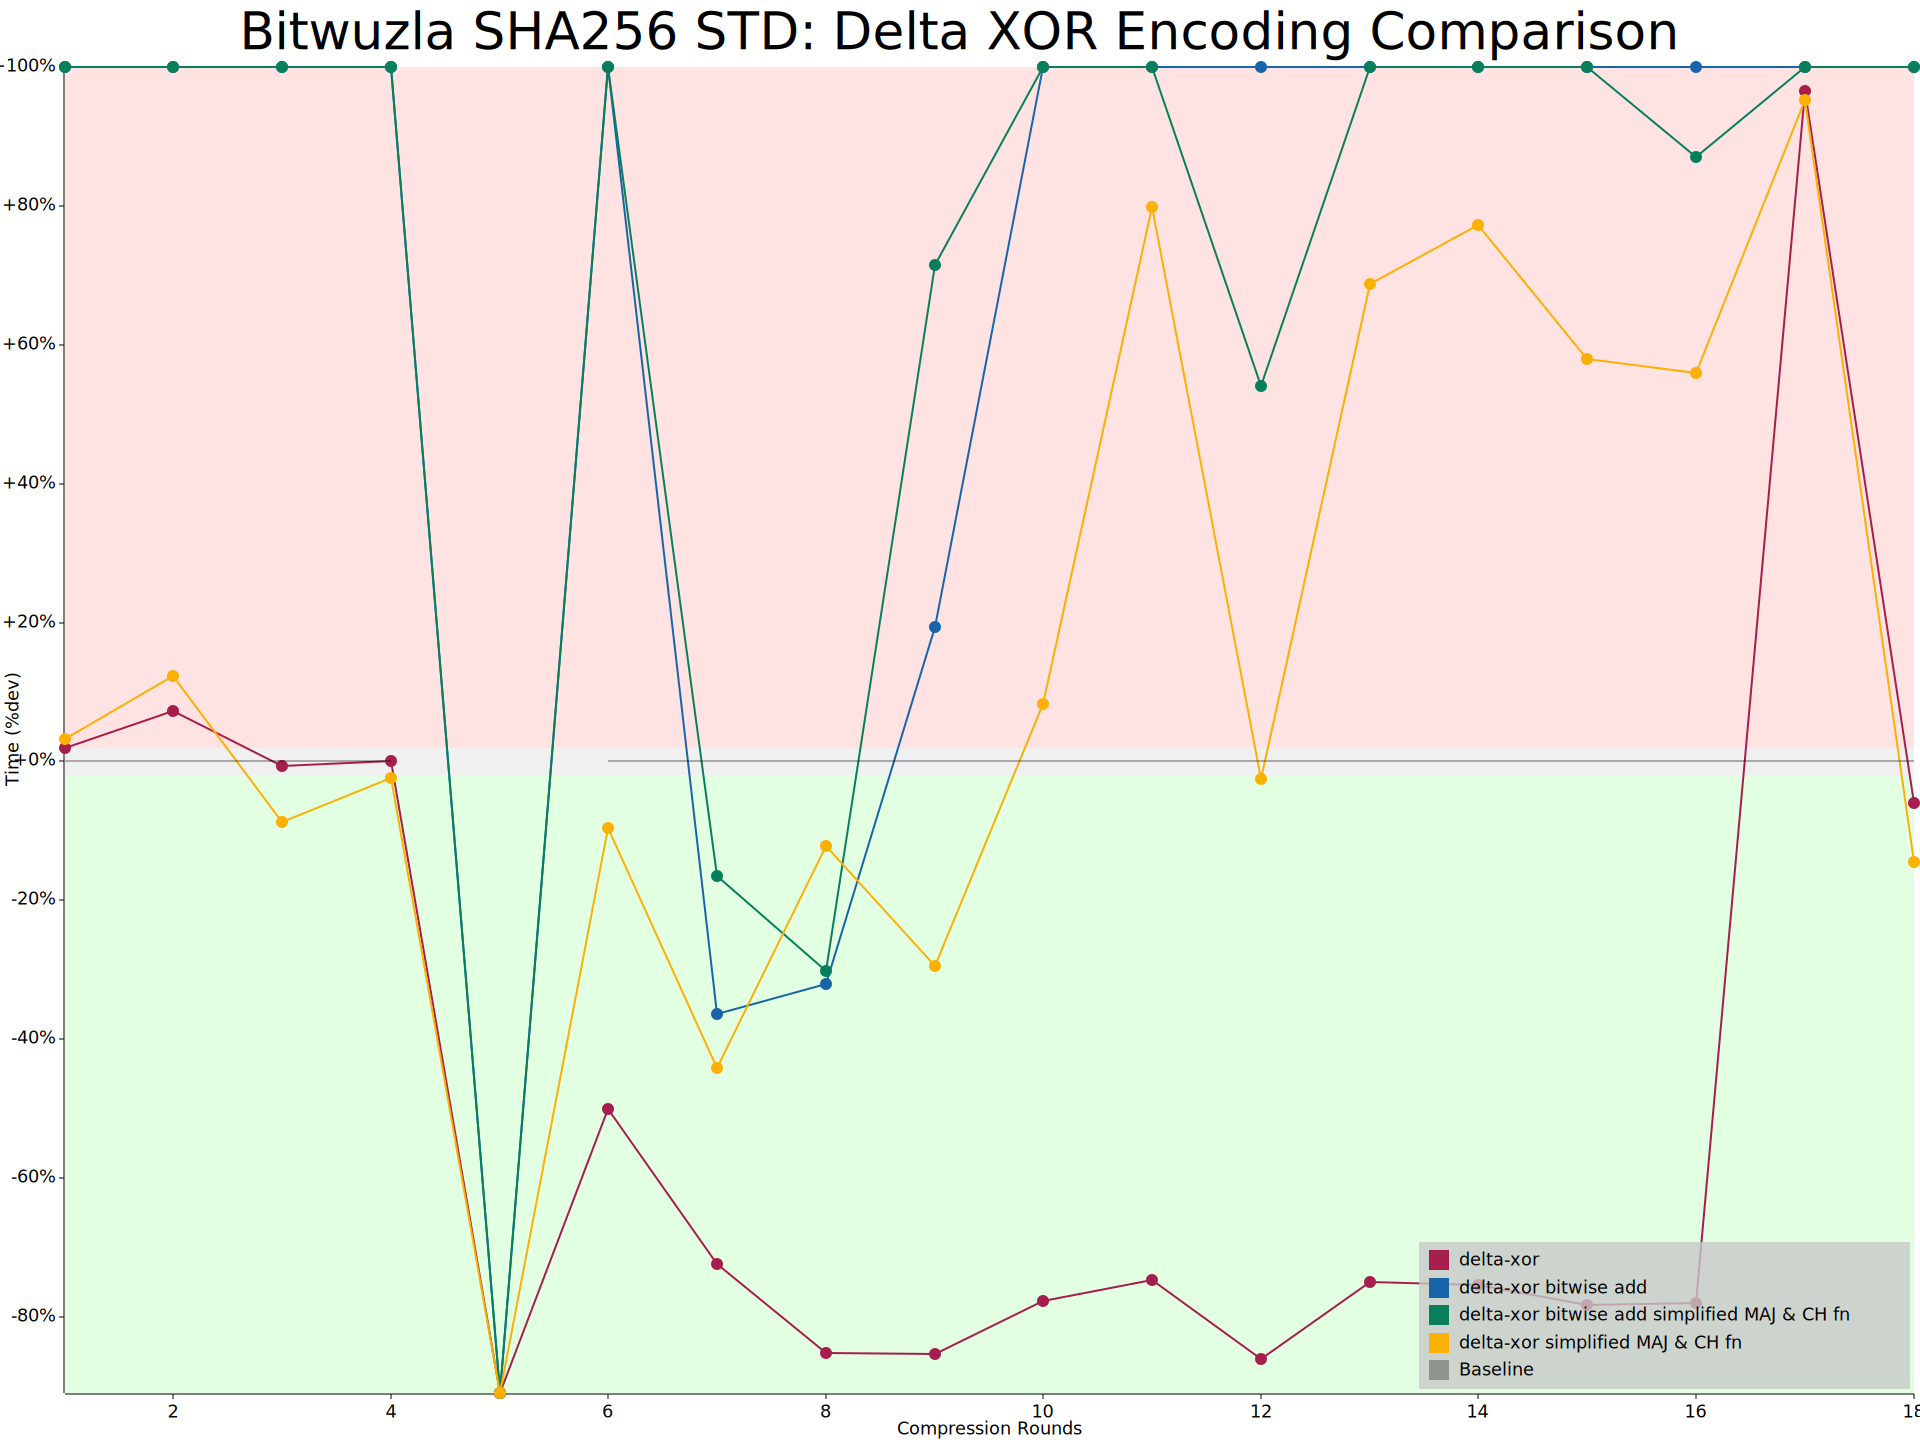
\includegraphics[width=0.8\textwidth]{../../graphs/bitwuzla_delta_xor_encoding_comparison.svg}
\end{figure}

\begin{figure}[H]
	\centering
	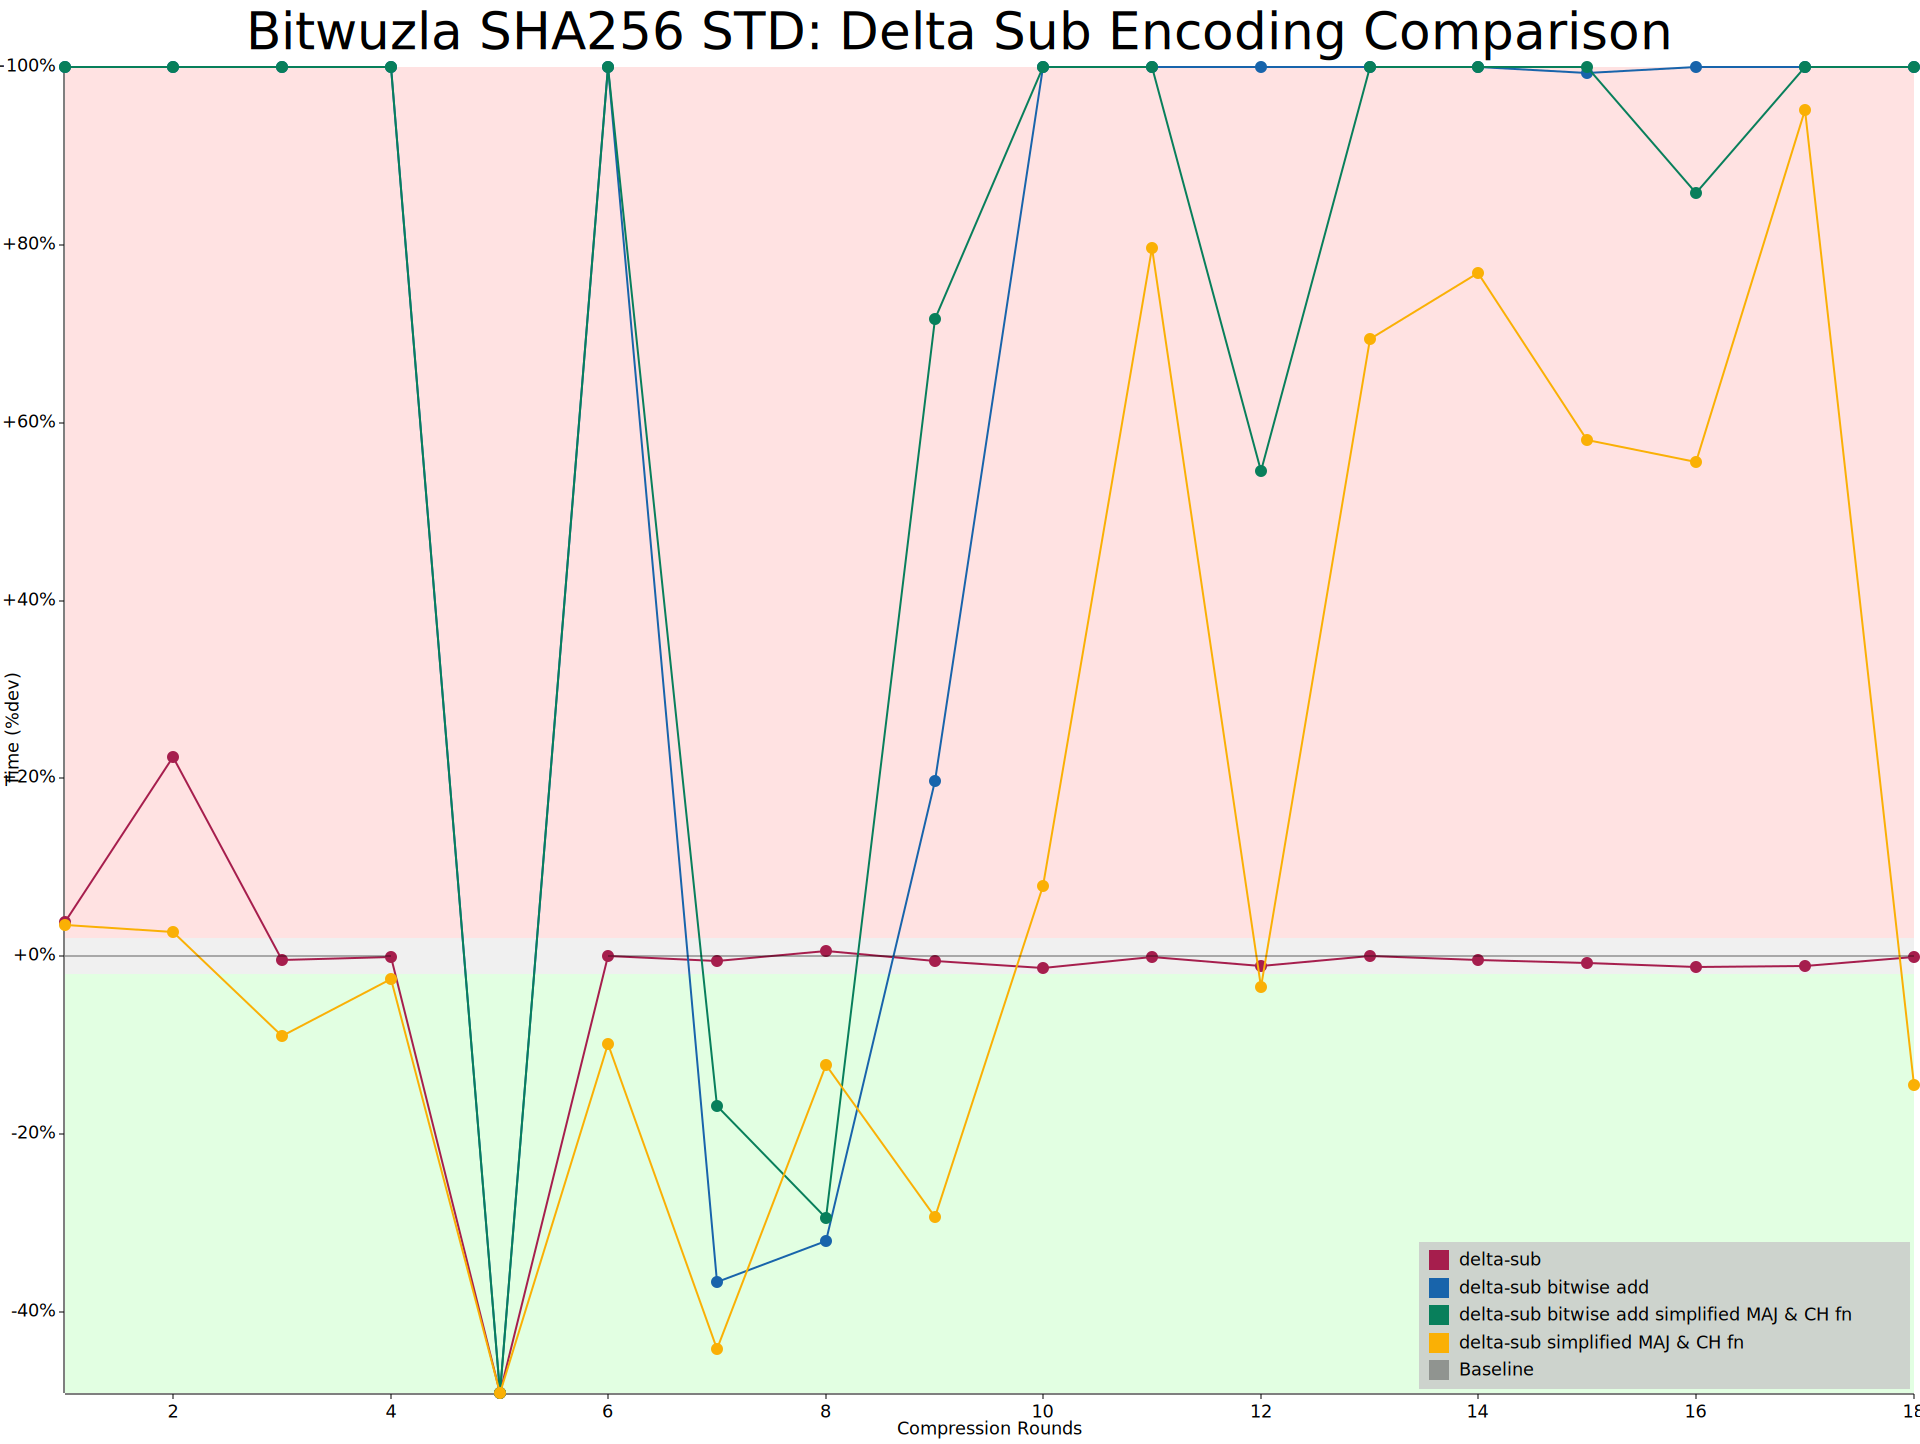
\includegraphics[width=0.8\textwidth]{../../graphs/bitwuzla_delta_sub_encoding_comparison.svg}
\end{figure}

	\begin{landscape}
\section{Result Tables}
\label{sec:full-results-tables}

\begin{table}[H]
\centering
\resizebox{1.5\textwidth}{!}{
\begin{tabular}{lllllllllllllllllllll}
Round & 1 & 2 & 3 & 4 & 5 & 6 & 7 & 8 & 9 & 10 & 11 & 12 & 13 & 14 & 15 & 16 & 17 & 18 & 19 & 20 \\
Time (s) & 0.0 & 0.0 & 0.7 & 2.2 & 3515.7 & 18.3 & 54.7 & 100.7 & 1.0 & 0.8 & 0.8 & 1.6 & 0.9 & 1.0 & 1.2 & 1.3 & 1.5 & 46.2 & 36000.1 & 900.1 \\
Memory (MiB) & 8258 & 9410 & 14082 & 21482 & 266754 & 46862 & 80986 & 100662 & 43066 & 47394 & 50894 & 57722 & 59262 & 61474 & 65806 & 73986 & 79482 & 100186 & - & - \\
Result & UNSAT & UNSAT & UNSAT & UNSAT & UNSAT & UNSAT & UNSAT & UNSAT & SAT & SAT & SAT & SAT & SAT & SAT & SAT & SAT & SAT & SAT & T/O & T/O \\
\end{tabular}}
\caption{Bitwuzla result table for standard collisions using brute-force encoding.}
\label{tab:bitwuzla-std-brute-force-results}
\end{table}

\begin{table}[H]
\centering
\resizebox{1.5\textwidth}{!}{
\begin{tabular}{lllllllllllllllllllll}
Round & 1 & 2 & 3 & 4 & 5 & 6 & 7 & 8 & 9 & 10 & 11 & 12 & 13 & 14 & 15 & 16 & 17 & 18 & 19 & 20 \\
Time (s) & 0.0 & 0.0 & 0.0 & 0.0 & 900.1 & 900.1 & 900.1 & 900.1 & 900.1 & 900.1 & 900.1 & 900.1 & 900.1 & 900.1 & 900.1 & 900.1 & 900.1 & 900.1 & 900.1 & 900.1 \\
Memory (MiB) & 28610 & 29378 & 29570 & 29570 & - & - & - & - & - & - & - & - & - & - & - & - & - & - & - & - \\
Result & UNSAT & UNSAT & UNSAT & UNSAT & T/O & T/O & T/O & T/O & T/O & T/O & T/O & T/O & T/O & T/O & T/O & T/O & T/O & T/O & T/O & T/O \\
\end{tabular}}
\caption{Z3 result table for standard collisions using brute-force encoding.}
\label{tab:z3-std-brute-force-results}
\end{table}

\begin{table}[H]
\centering
\resizebox{1.5\textwidth}{!}{
\begin{tabular}{lllllllllllllllllllll}
Round & 1 & 2 & 3 & 4 & 5 & 6 & 7 & 8 & 9 & 10 & 11 & 12 & 13 & 14 & 15 & 16 & 17 & 18 & 19 & 20 \\
Time (s) & 0.0 & 0.1 & 0.4 & 0.8 & 15.7 & 571.0 & 900.1 & 900.1 & 900.1 & 900.1 & 900.1 & 900.1 & 900.1 & 900.1 & 900.1 & 900.1 & 900.1 & 900.1 & 900.1 & 900.1 \\
Memory (MiB) & 4226 & 5186 & 6338 & 7682 & 23042 & 93890 & - & - & - & - & - & - & - & - & - & - & - & - & - & - \\
Result & UNSAT & UNSAT & UNSAT & UNSAT & UNSAT & UNSAT & T/O & T/O & T/O & T/O & T/O & T/O & T/O & T/O & T/O & T/O & T/O & T/O & T/O & T/O \\
\end{tabular}}
\caption{Yices result table for standard collisions using brute-force encoding.}
\label{tab:yices-std-brute-force-results}
\end{table}

\begin{table}[H]
\centering
\resizebox{1.5\textwidth}{!}{
\begin{tabular}{lllllllllllllllllllll}
Round & 1 & 2 & 3 & 4 & 5 & 6 & 7 & 8 & 9 & 10 & 11 & 12 & 13 & 14 & 15 & 16 & 17 & 18 & 19 & 20 \\
Time (s) & 0.0 & 0.1 & 0.4 & 0.9 & 900.1 & 900.1 & 900.1 & 900.1 & 900.1 & 900.1 & 900.1 & 900.1 & 900.1 & 900.1 & 900.1 & 900.1 & 900.1 & 900.1 & 900.1 & 900.1 \\
Memory (MiB) & 21506 & 27394 & 33062 & 41198 & - & - & - & - & - & - & - & - & - & - & - & - & - & - & - & - \\
Result & UNSAT & UNSAT & UNSAT & UNSAT & T/O & T/O & T/O & T/O & T/O & T/O & T/O & T/O & T/O & T/O & T/O & T/O & T/O & T/O & T/O & T/O \\
\end{tabular}}
\caption{CVC5 result table for standard collisions using brute-force encoding.}
\label{tab:cvc5-std-brute-force-results}
\end{table}

\begin{table}[H]
\centering
\resizebox{1.5\textwidth}{!}{
\begin{tabular}{lllllllllllllllllllll}
Round & 1 & 2 & 3 & 4 & 5 & 6 & 7 & 8 & 9 & 10 & 11 & 12 & 13 & 14 & 15 & 16 & 17 & 18 & 19 & 20 \\
Time (s) & 0.0 & 0.0 & 0.0 & 0.0 & 900.1 & 900.1 & 900.1 & 900.1 & 0.6 & 0.5 & 0.6 & 0.7 & 0.8 & 0.8 & 1.1 & 1.0 & 1.9 & 900.1 & 900.1 & 900.1 \\
Memory (MiB) & 10370 & 10562 & 10562 & 10754 & - & - & - & - & 40090 & 39598 & 43870 & 45514 & 49922 & 50306 & 53998 & 60650 & 68038 & - & - & - \\
Result & UNSAT & UNSAT & UNSAT & UNSAT & T/O & T/O & T/O & T/O & SAT & SAT & SAT & SAT & SAT & SAT & SAT & SAT & SAT & T/O & T/O & T/O \\
\end{tabular}}
\caption{MathSAT result table for standard collisions using brute-force encoding.}
\label{tab:mathsat-std-brute-force-results}
\end{table}

\begin{table}[H]
\centering
\resizebox{1.5\textwidth}{!}{
\begin{tabular}{llllllllllllllllll}
Round & 1 & 2 & 3 & 4 & 5 & 6 & 7 & 8 & 9 & 10 & 11 & 12 & 13 & 15 & 18 & 19 & 20 \\
Time (s) & 900.1 & 900.1 & 900.1 & 900.1 & 900.1 & 900.1 & 900.1 & 900.1 & 900.1 & 900.1 & 900.1 & 900.1 & 900.1 & 0.3 & 900.1 & 900.1 & 900.1 \\
Memory (MiB) & - & - & - & - & - & - & - & - & - & - & - & - & - & 33982 & - & - & - \\
Result & T/O & T/O & T/O & T/O & T/O & T/O & T/O & T/O & T/O & T/O & T/O & T/O & T/O & SAT & T/O & T/O & T/O \\
\end{tabular}}
\caption{Colibri2 result table for standard collisions using brute-force encoding.}
\label{tab:colibri2-std-brute-force-results}
\end{table}

\begin{table}[H]
\centering
\resizebox{1.5\textwidth}{!}{
\begin{tabular}{lllllllllllllllllllll}
Round & 1 & 2 & 3 & 4 & 5 & 6 & 7 & 8 & 9 & 10 & 11 & 12 & 13 & 14 & 15 & 16 & 17 & 18 & 19 & 20 \\
Time (s) & 0.0 & 0.0 & 900.1 & 900.1 & 900.1 & 900.1 & 900.1 & 900.1 & 900.1 & 900.1 & 900.1 & 900.1 & 31.4 & 56.6 & 30.0 & 48.4 & 57.9 & 900.1 & 900.1 & 900.1 \\
Memory (MiB) & 6146 & 6146 & - & - & - & - & - & - & - & - & - & - & 71562 & 98562 & 67390 & 84042 & 87206 & - & - & - \\
Result & UNSAT & UNSAT & T/O & T/O & T/O & T/O & T/O & T/O & T/O & T/O & T/O & T/O & SAT & SAT & SAT & SAT & SAT & T/O & T/O & T/O \\
\end{tabular}}
\caption{Boolector result table for standard collisions using brute-force encoding.}
\label{tab:boolector-std-brute-force-results}
\end{table}

\begin{table}[H]
\centering
\resizebox{1.5\textwidth}{!}{
\begin{tabular}{lllllllllllllllllllll}
Round & 1 & 2 & 3 & 4 & 5 & 6 & 7 & 8 & 9 & 10 & 11 & 12 & 13 & 14 & 15 & 16 & 17 & 18 & 19 & 20 \\
Time (s) & 0.9 & 2.9 & 5.4 & 6.4 & 21.0 & 66.9 & 34.6 & 68.4 & 1.2 & 2.7 & 1.9 & 3.4 & 3.7 & 2.3 & 2.4 & 4.1 & 5.8 & 362.3 & 900.1 & 900.1 \\
Memory (MiB) & 15142 & 22682 & 34802 & 42634 & 56926 & 106686 & 79210 & 115822 & 68262 & 79234 & 85202 & 88370 & 95298 & 102930 & 106790 & 116470 & 133174 & 242386 & - & - \\
Result & UNSAT & UNSAT & UNSAT & UNSAT & UNSAT & UNSAT & UNSAT & UNSAT & SAT & SAT & SAT & SAT & SAT & SAT & SAT & SAT & SAT & SAT & T/O & T/O \\
\end{tabular}}
\caption{Bitwuzla result table for standard collisions using brute-force encoding with alternative bitwise add.}
\label{tab:bitwuzla-std-brute-force-add-results}
\end{table}

\begin{table}[H]
\centering
\resizebox{1.5\textwidth}{!}{
\begin{tabular}{lllllllllllllllllllll}
Round & 1 & 2 & 3 & 4 & 5 & 6 & 7 & 8 & 9 & 10 & 11 & 12 & 13 & 14 & 15 & 16 & 17 & 18 & 19 & 20 \\
Time (s) & 0.0 & 0.0 & 0.6 & 2.1 & 11.2 & 16.5 & 30.5 & 88.2 & 0.7 & 0.8 & 1.4 & 1.5 & 1.6 & 1.7 & 1.9 & 2.0 & 3.0 & 39.4 & 900.1 & 900.1 \\
Memory (MiB) & 8066 & 9602 & 14214 & 21898 & 36646 & 44738 & 53554 & 100974 & 42670 & 46362 & 50462 & 53946 & 57698 & 64506 & 65374 & 70610 & 78422 & 107846 & - & - \\
Result & UNSAT & UNSAT & UNSAT & UNSAT & UNSAT & UNSAT & UNSAT & UNSAT & SAT & SAT & SAT & SAT & SAT & SAT & SAT & SAT & SAT & SAT & T/O & T/O \\
\end{tabular}}
\caption{Bitwuzla result table for standard collisions using brute-force encoding with simplified $Maj$ and $Ch$ functions.}
\label{tab:bitwuzla-std-brute-force-simpl-results}
\end{table}

\begin{table}[H]
\centering
\resizebox{1.5\textwidth}{!}{
\begin{tabular}{lllllllllllllllllllll}
Round & 1 & 2 & 3 & 4 & 5 & 6 & 7 & 8 & 9 & 10 & 11 & 12 & 13 & 14 & 15 & 16 & 17 & 18 & 19 & 20 \\
Time (s) & 0.9 & 2.9 & 5.4 & 6.5 & 22.1 & 70.5 & 45.5 & 70.5 & 1.8 & 3.5 & 1.9 & 2.4 & 3.7 & 2.3 & 4.2 & 2.4 & 10.2 & 356.0 & 900.1 & 900.1 \\
Memory (MiB) & 14970 & 23042 & 35358 & 40478 & 55666 & 105262 & 83890 & 123002 & 68954 & 77498 & 81406 & 87630 & 92902 & 103742 & 107810 & 114602 & 126794 & 282186 & - & - \\
Result & UNSAT & UNSAT & UNSAT & UNSAT & UNSAT & UNSAT & UNSAT & UNSAT & SAT & SAT & SAT & SAT & SAT & SAT & SAT & SAT & SAT & SAT & T/O & T/O \\
\end{tabular}}
\caption{Bitwuzla result table for standard collisions using brute-force encoding with simplified $Maj$ and $Ch$ functions, and alternative bitwise add.}
\label{tab:bitwuzla-std-brute-force-add-simpl-results}
\end{table}

\begin{table}[H]
\centering
\resizebox{1.5\textwidth}{!}{
\begin{tabular}{lllllllllllllllllllll}
Round & 1 & 2 & 3 & 4 & 5 & 6 & 7 & 8 & 9 & 10 & 11 & 12 & 13 & 14 & 15 & 16 & 17 & 18 & 19 & 20 \\
Time (s) & 0.9 & 2.9 & 5.4 & 6.4 & 21.0 & 67.1 & 34.8 & 68.3 & 1.2 & 2.7 & 1.9 & 3.4 & 3.7 & 2.3 & 2.4 & 4.1 & 5.9 & 361.8 & 900.1 & 900.1 \\
Memory (MiB) & 14910 & 25158 & 35174 & 41354 & 56822 & 112482 & 81246 & 118758 & 69246 & 79494 & 84626 & 89470 & 95594 & 106794 & 114206 & 116626 & 132430 & 240878 & - & - \\
Result & UNSAT & UNSAT & UNSAT & UNSAT & UNSAT & UNSAT & UNSAT & UNSAT & SAT & SAT & SAT & SAT & SAT & SAT & SAT & SAT & SAT & SAT & T/O & T/O \\
\end{tabular}}
\caption{Bitwuzla result table for standard collisions using delta XOR encoding with alternative bitwise add.}
\label{tab:bitwuzla-std-delta-xor-add-results}
\end{table}

\begin{table}[H]
\centering
\resizebox{1.5\textwidth}{!}{
\begin{tabular}{lllllllllllllllllllll}
Round & 1 & 2 & 3 & 4 & 5 & 6 & 7 & 8 & 9 & 10 & 11 & 12 & 13 & 14 & 15 & 16 & 17 & 18 & 19 & 20 \\
Time (s) & 0.0 & 0.0 & 0.6 & 2.1 & 11.3 & 16.6 & 30.5 & 88.4 & 0.7 & 0.8 & 1.4 & 1.5 & 1.6 & 1.7 & 1.9 & 2.0 & 3.0 & 39.5 & 900.1 & 900.1 \\
Memory (MiB) & 8066 & 9410 & 15050 & 22922 & 36534 & 44286 & 55890 & 103570 & 42950 & 46390 & 51910 & 53990 & 57538 & 64138 & 65426 & 70958 & 76566 & 102770 & - & - \\
Result & UNSAT & UNSAT & UNSAT & UNSAT & UNSAT & UNSAT & UNSAT & UNSAT & SAT & SAT & SAT & SAT & SAT & SAT & SAT & SAT & SAT & SAT & T/O & T/O \\
\end{tabular}}
\caption{Bitwuzla result table for standard collisions using delta XOR encoding with simplified $Maj$ and $Ch$ functions.}
\label{tab:bitwuzla-std-delta-xor-simpl-results}
\end{table}

\begin{table}[H]
\centering
\resizebox{1.5\textwidth}{!}{
\begin{tabular}{lllllllllllllllllllll}
Round & 1 & 2 & 3 & 4 & 5 & 6 & 7 & 8 & 9 & 10 & 11 & 12 & 13 & 14 & 15 & 16 & 17 & 18 & 19 & 20 \\
Time (s) & 0.9 & 2.9 & 5.4 & 6.5 & 22.2 & 70.3 & 45.6 & 70.2 & 1.8 & 3.5 & 1.9 & 2.4 & 3.7 & 2.3 & 4.2 & 2.4 & 10.2 & 352.8 & 900.1 & 900.1 \\
Memory (MiB) & 14954 & 22870 & 36734 & 39682 & 56962 & 103294 & 85238 & 117686 & 69726 & 77530 & 81894 & 87786 & 92934 & 103886 & 111798 & 114642 & 123514 & 282870 & - & - \\
Result & UNSAT & UNSAT & UNSAT & UNSAT & UNSAT & UNSAT & UNSAT & UNSAT & SAT & SAT & SAT & SAT & SAT & SAT & SAT & SAT & SAT & SAT & T/O & T/O \\
\end{tabular}}
\caption{Bitwuzla result table for standard collisions using delta XOR encoding with simplified $Maj$ and $Ch$ functions, and alternative bitwise add.}
\label{tab:bitwuzla-std-delta-xor-add-simpl-results}
\end{table}

\begin{table}[H]
\centering
\resizebox{1.5\textwidth}{!}{
\begin{tabular}{lllllllllllllllllllll}
Round & 1 & 2 & 3 & 4 & 5 & 6 & 7 & 8 & 9 & 10 & 11 & 12 & 13 & 14 & 15 & 16 & 17 & 18 & 19 & 20 \\
Time (s) & 0.0 & 0.0 & 0.7 & 2.2 & 900.1 & 18.3 & 54.4 & 101.2 & 1.0 & 0.8 & 0.8 & 1.6 & 0.9 & 1.0 & 1.2 & 1.3 & 1.5 & 46.2 & 900.1 & 900.1 \\
Memory (MiB) & 8258 & 9218 & 14386 & 22938 & - & 47222 & 80618 & 100766 & 43286 & 47134 & 51994 & 55050 & 64386 & 61514 & 67266 & 71586 & 80502 & 103022 & - & - \\
Result & UNSAT & UNSAT & UNSAT & UNSAT & T/O & UNSAT & UNSAT & UNSAT & SAT & SAT & SAT & SAT & SAT & SAT & SAT & SAT & SAT & SAT & T/O & T/O \\
\end{tabular}}
\caption{Bitwuzla result table for standard collisions using delta Sub encoding.}
\label{tab:bitwuzla-std-delta-sub-results}
\end{table}

\begin{table}[H]
\centering
\resizebox{1.5\textwidth}{!}{
\begin{tabular}{lllllllllllllllllllll}
Round & 1 & 2 & 3 & 4 & 5 & 6 & 7 & 8 & 9 & 10 & 11 & 12 & 13 & 14 & 15 & 16 & 17 & 18 & 19 & 20 \\
Time (s) & 0.9 & 2.9 & 5.4 & 6.4 & 21.0 & 66.9 & 34.6 & 68.4 & 1.2 & 2.7 & 1.9 & 3.4 & 3.7 & 2.3 & 2.4 & 4.1 & 5.8 & 361.9 & 900.1 & 900.1 \\
Memory (MiB) & 14946 & 25358 & 34334 & 39762 & 56798 & 91638 & 84022 & 117454 & 69234 & 78310 & 85198 & 88210 & 94246 & 102958 & 114958 & 116706 & 130694 & 239462 & - & - \\
Result & UNSAT & UNSAT & UNSAT & UNSAT & UNSAT & UNSAT & UNSAT & UNSAT & SAT & SAT & SAT & SAT & SAT & SAT & SAT & SAT & SAT & SAT & T/O & T/O \\
\end{tabular}}
\caption{Bitwuzla result table for standard collisions using delta Sub encoding with alternative bitwise add.}
\label{tab:bitwuzla-std-delta-sub-add-results}
\end{table}

\begin{table}[H]
\centering
\resizebox{1.5\textwidth}{!}{
\begin{tabular}{lllllllllllllllllllll}
Round & 1 & 2 & 3 & 4 & 5 & 6 & 7 & 8 & 9 & 10 & 11 & 12 & 13 & 14 & 15 & 16 & 17 & 18 & 19 & 20 \\
Time (s) & 0.0 & 0.0 & 0.6 & 2.1 & 11.3 & 16.5 & 30.5 & 88.3 & 0.7 & 0.8 & 1.4 & 1.5 & 1.6 & 1.7 & 1.9 & 2.0 & 3.0 & 39.6 & 900.1 & 900.1 \\
Memory (MiB) & 8450 & 9602 & 13822 & 23038 & 41230 & 42910 & 55442 & 94750 & 42422 & 47602 & 51038 & 53902 & 57954 & 64262 & 63514 & 69850 & 77074 & 107982 & - & - \\
Result & UNSAT & UNSAT & UNSAT & UNSAT & UNSAT & UNSAT & UNSAT & UNSAT & SAT & SAT & SAT & SAT & SAT & SAT & SAT & SAT & SAT & SAT & T/O & T/O \\
\end{tabular}}
\caption{Bitwuzla result table for standard collisions using delta Sub encoding with simplified $Maj$ and $Ch$ functions.}
\label{tab:bitwuzla-std-delta-sub-simpl-results}
\end{table}

\begin{table}[H]
\centering
\resizebox{1.5\textwidth}{!}{
\begin{tabular}{lllllllllllllllllllll}
Round & 1 & 2 & 3 & 4 & 5 & 6 & 7 & 8 & 9 & 10 & 11 & 12 & 13 & 14 & 15 & 16 & 17 & 18 & 19 & 20 \\
Time (s) & 0.9 & 2.9 & 5.4 & 6.5 & 22.1 & 70.7 & 45.5 & 71.0 & 1.8 & 3.5 & 1.9 & 2.4 & 3.7 & 2.3 & 4.2 & 2.4 & 10.2 & 354.8 & 900.1 & 900.1 \\
Memory (MiB) & 15066 & 23026 & 36178 & 43438 & 57914 & 106126 & 83238 & 123038 & 69950 & 77426 & 81874 & 88110 & 93382 & 100990 & 105074 & 114586 & 129902 & 283446 & - & - \\
Result & UNSAT & UNSAT & UNSAT & UNSAT & UNSAT & UNSAT & UNSAT & UNSAT & SAT & SAT & SAT & SAT & SAT & SAT & SAT & SAT & SAT & SAT & T/O & T/O \\
\end{tabular}}
\caption{Bitwuzla result table for standard collisions using delta Sub encoding with simplified $Maj$ and $Ch$ functions, and alternative bitwise add.}
\label{tab:bitwuzla-std-delta-sub-add-simpl-results}
\end{table}
\end{landscape}



	\chapter{Source Code}
	\section{Notes}
This tex document makes use of the lstlisting-rust provided under the BSD-3 licence. \cite{lstlisting-rust}

\section{Proofs}
\subsection{Bitwise Adder}
\begin{lstlisting}[language=Lisp, caption={Core adder in SMTLIB2 for 32-bit BV}, label=lst:bitadd]
(define-fun bitadd-2 ((a (_ BitVec 32)) (b (_ BitVec 32))) (_ BitVec 32)
	(let (
		(p0 (bvxor a b))
		(g0 (bvand a b))
	)
	(
		let (
			(g1 (bvor g0 (bvand p0 (bvshl g0 #x00000001))))
			(p1 (bvand p0 (bvshl p0 #x00000001)))
		)
		(
			let (
				(g2 (bvor g1 (bvand p1 (bvshl g1 #x00000002))))
				(p2 (bvand p1 (bvshl p1 #x00000002)))
			)
			(
				let (
					(g3 (bvor g2 (bvand p2 (bvshl g2 #x00000004))))
					(p3 (bvand p2 (bvshl p2 #x00000004)))
				)
				(
					let (
						(g4 (bvor g3 (bvand p3 (bvshl g3 #x00000008))))
						(p4 (bvand p3 (bvshl p3 #x00000008)))
					)
					(
						let (
							(g5 (bvor g4 (bvand p4 (bvshl g4 #x00000010))))
							(p5 (bvand p4 (bvshl p4 #x00000010)))
						)
						(
							let (
								(g6 (bvor g5 (bvand p5 (bvshl g5 #x00000020))))
								(p6 (bvand p5 (bvshl p5 #x00000020))) ; Redundant
							)
							(
								bvxor p0 (bvshl g6 #x00000001)
							)
						)
					)
				)
			)
		)
	))
)
\end{lstlisting}

\begin{lstlisting}[language=lisp, caption={multiple operand adder in smtlib2 for 32-bit bv}, label=lst:bitadd-multi]
(define-fun bitadd-3 ((a (_ bitvec 32)) (b (_ bitvec 32)) (c (_ bitvec 32))) (_ bitvec 32)
	(let (
		(sum (bvxor a b c))
		(carry (bvshl (bvor (bvand a b) (bvand a c) (bvand b c)) #x00000001))
	)
	(
		bitadd-2 sum carry
	))
)
(define-fun bitadd-4 ((a (_ bitvec 32)) (b (_ bitvec 32)) (c (_ bitvec 32)) (d (_ bitvec 32))) (_ bitvec 32)
	(let (
		(sum (bvxor a b c))
		(carry (bvshl (bvor (bvand a b) (bvand a c) (bvand b c)) #x00000001))
	)
	(
		bitadd-3 sum carry d
	))
)
(define-fun bitadd-5 ((a (_ bitvec 32)) (b (_ bitvec 32)) (c (_ bitvec 32)) (d (_ bitvec 32)) (e (_ bitvec 32))) (_ bitvec 32)
	(let (
		(sum1 (bvxor a b c))
		(carry1 (bvshl (bvor (bvand a b) (bvand a c) (bvand b c)) #x00000001))
		(sum2 (bvxor d e))
		(carry2 (bvshl (bvand d e) #x00000001))
	)
	(
		bitadd-4 sum1 carry1 sum2 carry2
	))
)
(define-fun bitadd-6 ((a (_ bitvec 32)) (b (_ bitvec 32)) (c (_ bitvec 32)) (d (_ bitvec 32)) (e (_ bitvec 32)) (f (_ bitvec 32))) (_ bitvec 32)
	(let (
		(sum1 (bvxor a b c))
		(carry1 (bvshl (bvor (bvand a b) (bvand a c) (bvand b c)) #x00000001))
		(sum2 (bvxor d e f))
		(carry2 (bvshl (bvor (bvand d e) (bvand d f) (bvand e f)) #x00000001))
	)
	(
		bitadd-4 sum1 carry1 sum2 carry2
	))
)
\end{lstlisting}

\subsection{BASE4 Proofs}
\begin{lstlisting}[language=lisp, caption={AND logic proof}, label=lst:and-proof]
(set-option :produce-models true)
(set-logic QF_BV)

(define-sort BV4 () (_ BitVec 4))


; Input Variables
(declare-fun LEFT_X () BV4)
(declare-fun RIGHT_X () BV4)
(declare-fun LEFT_Y () BV4)
(declare-fun RIGHT_Y () BV4)


; Differential variables for X
(define-fun X_a () BV4 (bvand (bvnot LEFT_X) (bvnot RIGHT_X)))
(define-fun X_b () BV4 (bvand (bvnot LEFT_X) RIGHT_X))
(define-fun X_c () BV4 (bvand LEFT_X (bvnot RIGHT_X)))
(define-fun X_d () BV4 (bvand LEFT_X RIGHT_X))
(define-fun X_f () BV4 (bvor X_b X_d))  ; f = b OR d
(define-fun X_g () BV4 (bvor X_c X_d))  ; g = c OR d


; Differential variables for Y
(define-fun Y_a () BV4 (bvand (bvnot LEFT_Y) (bvnot RIGHT_Y)))
(define-fun Y_b () BV4 (bvand (bvnot LEFT_Y) RIGHT_Y))
(define-fun Y_c () BV4 (bvand LEFT_Y (bvnot RIGHT_Y)))
(define-fun Y_d () BV4 (bvand LEFT_Y RIGHT_Y))
(define-fun Y_f () BV4 (bvor Y_b Y_d))  ; f = b OR d
(define-fun Y_g () BV4 (bvor Y_c Y_d))  ; g = c OR d


; Theory Diff
(define-fun LEFT_XY () BV4 (bvand LEFT_X LEFT_Y))
(define-fun RIGHT_XY () BV4 (bvand RIGHT_X RIGHT_Y))


; Actual
(define-fun a_XY () BV4 (bvand (bvnot LEFT_XY) (bvnot RIGHT_XY)))
(define-fun b_XY () BV4 (bvand (bvnot LEFT_XY) RIGHT_XY))
(define-fun c_XY () BV4 (bvand LEFT_XY (bvnot RIGHT_XY)))
(define-fun d_XY () BV4 (bvand LEFT_XY RIGHT_XY))


; Logic
(define-fun d2 () BV4 (bvand X_d Y_d))
(define-fun b2 () BV4 (bvand (bvand X_f Y_f) (bvnot d2)))
(define-fun c2 () BV4 (bvand (bvand X_g Y_g) (bvnot d2)))
(define-fun a2 () BV4 (bvnot (bvor d2 (bvor c2 b2))))


; Assert mismatch
(assert (not (and
		(= a2 a_XY)
		(= b2 b_XY)
		(= c2 c_XY)
		(= d2 d_XY)
)))


(check-sat)
\end{lstlisting}

\begin{lstlisting}[language=lisp, caption={OR logic proof}, label=lst:or-proof]
(set-option :produce-models true)
(set-logic QF_BV)

(define-sort BV4 () (_ BitVec 4))


; Input Variables
(declare-fun LEFT_X () BV4)
(declare-fun RIGHT_X () BV4)
(declare-fun LEFT_Y () BV4)
(declare-fun RIGHT_Y () BV4)


; Differential variables for X
(define-fun X_a () BV4 (bvand (bvnot LEFT_X) (bvnot RIGHT_X)))
(define-fun X_b () BV4 (bvand (bvnot LEFT_X) RIGHT_X))
(define-fun X_c () BV4 (bvand LEFT_X (bvnot RIGHT_X)))
(define-fun X_d () BV4 (bvand LEFT_X RIGHT_X))
(define-fun X_f () BV4 (bvor X_b X_d))  ; f = b OR d
(define-fun X_g () BV4 (bvor X_c X_d))  ; g = c OR d


; Differential variables for Y
(define-fun Y_a () BV4 (bvand (bvnot LEFT_Y) (bvnot RIGHT_Y)))
(define-fun Y_b () BV4 (bvand (bvnot LEFT_Y) RIGHT_Y))
(define-fun Y_c () BV4 (bvand LEFT_Y (bvnot RIGHT_Y)))
(define-fun Y_d () BV4 (bvand LEFT_Y RIGHT_Y))
(define-fun Y_f () BV4 (bvor Y_b Y_d))  ; f = b OR d
(define-fun Y_g () BV4 (bvor Y_c Y_d))  ; g = c OR d


; Theory Diff
(define-fun LEFT_XY () BV4 (bvor LEFT_X LEFT_Y))
(define-fun RIGHT_XY () BV4 (bvor RIGHT_X RIGHT_Y))


; Actual
(define-fun a_XY () BV4 (bvand (bvnot LEFT_XY) (bvnot RIGHT_XY)))
(define-fun b_XY () BV4 (bvand (bvnot LEFT_XY) RIGHT_XY))
(define-fun c_XY () BV4 (bvand LEFT_XY (bvnot RIGHT_XY)))
(define-fun d_XY () BV4 (bvand LEFT_XY RIGHT_XY))


; Logic
(define-fun a2 () BV4 (bvand X_a Y_a))
(define-fun b2 () BV4 (bvnot (bvor X_g Y_g a2)))
(define-fun c2 () BV4 (bvnot (bvor X_f Y_f a2)))
(define-fun d2 () BV4 (bvnot (bvor a2 b2 c2)))


; Assert mismatch
(assert (not (and
		(= a2 a_XY)
		(= b2 b_XY)
		(= c2 c_XY)
		(= d2 d_XY)
)))


(check-sat)
\end{lstlisting}

\begin{lstlisting}[language=lisp, caption={XOR logic proof}, label=lst:xor-proof]
(set-option :produce-models true)
(set-logic QF_BV)

(define-sort BV4 () (_ BitVec 4))


; Input variables
(declare-fun LEFT_X () BV4)
(declare-fun RIGHT_X () BV4)
(declare-fun LEFT_Y () BV4)
(declare-fun RIGHT_Y () BV4)


; Differential variables for X
(define-fun X_a () BV4 (bvand (bvnot LEFT_X) (bvnot RIGHT_X)))
(define-fun X_b () BV4 (bvand (bvnot LEFT_X) RIGHT_X))
(define-fun X_c () BV4 (bvand LEFT_X (bvnot RIGHT_X)))
(define-fun X_d () BV4 (bvand LEFT_X RIGHT_X))


; Differential variables for Y
(define-fun Y_a () BV4 (bvand (bvnot LEFT_Y) (bvnot RIGHT_Y)))
(define-fun Y_b () BV4 (bvand (bvnot LEFT_Y) RIGHT_Y))
(define-fun Y_c () BV4 (bvand LEFT_Y (bvnot RIGHT_Y)))
(define-fun Y_d () BV4 (bvand LEFT_Y RIGHT_Y))


; Theory Diff
(define-fun LEFT_XY () BV4 (bvxor LEFT_X LEFT_Y))
(define-fun RIGHT_XY () BV4 (bvxor RIGHT_X RIGHT_Y))


; Actual
(define-fun a_XY () BV4 (bvand (bvnot LEFT_XY) (bvnot RIGHT_XY)))
(define-fun b_XY () BV4 (bvand (bvnot LEFT_XY) RIGHT_XY))
(define-fun c_XY () BV4 (bvand LEFT_XY (bvnot RIGHT_XY)))
(define-fun d_XY () BV4 (bvand LEFT_XY RIGHT_XY))


; Logic
(define-fun a2 () BV4
		(bvor (bvand X_a Y_a)
					(bvand X_b Y_b)
					(bvand X_c Y_c)
					(bvand X_d Y_d)
		)
)

(define-fun b2 () BV4
		(bvor (bvand X_a Y_b)
					(bvand X_b Y_a)
					(bvand X_c Y_d)
					(bvand X_d Y_c)
		)
)

(define-fun c2 () BV4
		(bvor (bvand X_a Y_c)
					(bvand X_c Y_a)
					(bvand X_b Y_d)
					(bvand X_d Y_b)
		)
)

(define-fun d2 () BV4
		(bvor (bvand X_a Y_d)
					(bvand X_d Y_a)
					(bvand X_b Y_c)
					(bvand X_c Y_b)
		)
)


; Assert mismatch
(assert (not (and
		(= a2 a_XY)
		(= b2 b_XY)
		(= c2 c_XY)
		(= d2 d_XY)
)))

(check-sat)
\end{lstlisting}

\section{Rust Codebase}
\label{sec:codebase}
\begin{lstlisting}[language=rust, caption={main.rs}]
use std::error::Error;
use std::fs;
use std::ops::Range;
use std::path::PathBuf;
use std::time::Duration;
use clap::{Parser, Subcommand};
use plotters::prelude::RGBColor;
use crate::benchmark::runner::BenchmarkRunner;
use crate::data::data_retriever::DataRetriever;
use crate::graphing::graph_renderer::GraphRenderer;
use crate::sha::{MessageBlock, Sha, StartVector, Word};
use crate::smt_lib::smt_lib::generate_smtlib_files;
use crate::smt_lib::smt_retriever::{EncodingType, SmtRetriever};
use crate::structs::benchmark::{Benchmark, SmtSolver};
use crate::structs::collision_type::CollisionType;
use crate::structs::hash_function::HashFunction;

#[cfg(not(unix))]
compile_error!("This crate supports only Unix-like operating systems");

mod smt_lib;
mod sha;
mod verification;
mod structs;
mod graphing;
mod data;
mod benchmark;


#[derive(Parser, Debug)]
#[command(author, version, about, long_about = None)]
struct Cli {
	#[command(subcommand)]
	command: Commands,
}

#[derive(Subcommand, Debug)]
enum Commands {
	/// Generate SMTLIB 2.6 standard files
	Generate {
		/// Directory where smt2 files will be saved. Default `smt/`
		#[arg(short = 'S', long)]
		smt_dir: Option<PathBuf>,
	},

	/// Run an exhaustive benchmark over all solvers, hash functions, collision types and arguments
	Benchmark {
		/// Argument to select solver. Use multiple `--solver <SOLVER>` statements for multiple solvers
		#[arg(required = true, long)]
		solver: Vec<SmtSolver>,

		/// Argument to select hash function. Use separate `--hash-function <HASH_FUNCTION>` statements for multiple hash functions
		#[arg(required = true, long)]
		hash_function: Vec<HashFunction>,

		/// Argument to select collision type. Use separate `--collision-type <COLLISION_TYPE>` statements for multiple collision types
		#[arg(required = true, long)]
		collision_type: Vec<CollisionType>,

		/// Argument to set (non-inclusive) range of compression rounds. Input with `--round-range <MIN>..<MAX>`. Default 1..hash function max
		#[arg(long, value_parser = parse_range)]
		round_range: Option<Range<u8>>,

		/// Argument to set the solver argument sets (combinations of solver arguments).
		/// An arugment set can contain multiple arguments which will all be executed on the solver.
		/// To test each argument separately, set each solver argument as a separate --arg-set.
		/// Use separate `--arg-set "<ARG_SET>"` statements for multiple argument sets.
		/// Default <No Args>
		#[arg(long, allow_hyphen_values = true)]
		arg_set: Option<Vec<String>>,

		/// The number of required sequential failures to stop. Default 3
		#[arg(short, long)]
		stop_tolerance:  Option<u8>,

		/// Duration after which run is marked as timed out. Default 15 mins
		#[arg(short, long)]
		timeout_sec: Option<u64>,

		/// Path to directory containing SMT files. Default `smt/`
		#[arg(short = 'S', long)]
		smt_dir: Option<PathBuf>,

		/// Path to directory where result files will be saved to. `None` to disable output. Default `results/`
		#[arg(short, long)]
		result_dir: Option<PathBuf>,

		/// Should remaining benchmark runs continue despite error on one. Default false
		#[arg(short = 'C', visible_alias = "cof", long)]
		continue_on_fail: Option<bool>,

		/// Type of encoding to benchmark.
		/// Format `<encoding_type>:[simplified_maj_and_ch_functions]:[alternative_add]`,
		/// where simplified_maj_and_ch_functions and alternative_add are bool with default false.
		///
		/// Valid examples: `bruteforce:true:true`, `dxor::true`, `base4:true`, `dsub`.
		/// Default bruteforce:false:false
		///
		/// [encoding_type possible values: bruteforce, dxor, dsub, base4]
		#[arg(short = 'E', long)]
		encoding_type: Option<String>,

		/// Should the benchmark be marked as a rerun. Useful for flagging up anomalies. Default false
		#[arg(short = 'R', long)]
		is_rerun: Option<bool>,
	},

	/// Run the underlying sha2 function
	Sha2 {
		/// Message to hash
		#[arg(short, long)]
		msg: Option<String>,

		/// Message digest block to hash (pre-padded and pre-processed digest), separated word-by-word with spaces
		#[arg(short = 'M', visible_alias = "mb", long)]
		msg_block: Option<String>,

		/// Hash function
		hash_function: HashFunction,

		/// Number of compression rounds. Default hash function max
		#[arg(short, long)]
		rounds: Option<u8>,

		/// Starting vector for hash function, separated word-by-word with spaces. Default Initial Vector (IV)
		#[arg(long, visible_alias = "sv")]
		start_vector: Option<String>,
	},

	/// Load, verify and display result files
	Load {
		/// Path to a result file, or a directory. Default `results/`
		#[arg(short = 'R', long)]
		result_path: Option<PathBuf>,

		/// Should directory scan be recursive. Default true
		#[arg(short, long)]
		recursive: Option<bool>,
	},

	/// Render result graphs
	Graph {
		/// Directory where graphs will be saved. Default `graphs/`
		#[arg(long)]
		graph_dir: Option<PathBuf>,

		/// Directory where all benchmark results are stored. Default `results/`
		#[arg(long)]
		result_dir: Option<PathBuf>,
	}
}

fn main() -> Result<(), Box<dyn Error>> {
	let cli = Cli::parse();

	match &cli.command {
		Commands::Generate { smt_dir } => {
			let smt_dir = smt_dir.clone().unwrap_or(PathBuf::from("smt/"));
			generate_smtlib_files(
				SmtRetriever::new(smt_dir)?
			)?;
		},

		Commands::Benchmark {
			solver: solvers,
			hash_function: hash_functions,
			collision_type: collision_types,
			round_range,
			arg_set,
			stop_tolerance,
			timeout_sec,
			smt_dir,
			result_dir,
			continue_on_fail,
			encoding_type,
			is_rerun,
		} => {
			let round_range = round_range.clone().unwrap_or(1..80);
			let arg_set = arg_set.clone().unwrap_or(Vec::with_capacity(0));
			let stop_tolerance = (*stop_tolerance).unwrap_or(3);
			let timeout = Duration::from_secs((*timeout_sec).unwrap_or(15 * 60));
			let continue_on_fail = (*continue_on_fail).unwrap_or(false);
			let encoding_type: EncodingType = encoding_type.as_deref().map_or(
				EncodingType::BruteForce {
					simplified_maj_and_ch_functions: false,
					alternative_add: false,
				},
				|s| s.parse().expect("Failed to parse encoding type")
			);
			let smt_dir = smt_dir.clone().unwrap_or(PathBuf::from("smt/"));
			let is_rerun = is_rerun.unwrap_or(false);

			let save_dir = if result_dir
				.clone()
				.is_some_and(|path| path.to_str().unwrap().to_lowercase() == "none")
			{
				None
			} else if let Some(path) = result_dir.clone() {
				Some(path)
			} else {
				Some(PathBuf::from("results/"))
			};

			let runner = BenchmarkRunner::new(
				stop_tolerance,
				timeout,
				SmtRetriever::new(smt_dir)?,
				save_dir,
				continue_on_fail,
				encoding_type,
				is_rerun,
			);

			runner.run_benchmarks(
				solvers.clone(),
				hash_functions.clone(),
				collision_types.clone(),
				round_range,
				arg_set,
			)?;
		}

		Commands::Sha2 {
			msg,
			msg_block,
			hash_function,
			rounds,
			start_vector,
		} => {
			let rounds = rounds.unwrap_or(hash_function.max_rounds());

			let start_vector = match start_vector {
				None => StartVector::IV,
				Some(start_vector) => {
					let mut words= Vec::with_capacity(8);
					for word in start_vector.split_whitespace() {
						words.push(Word::from_str_radix(word, 16, *hash_function)?);
					}

					StartVector::CV(<[Word; 8]>::try_from(words).unwrap())
				}
			};

			let result = if let Some(msg) = msg {
				Sha::from_string(
					msg,
					*hash_function,
					rounds,
					start_vector,
				)?.execute()?
			} else if let Some(msg_block) = msg_block {
				Sha::from_message_block(
					MessageBlock::from_str_radix(msg_block, 16, *hash_function)?,
					*hash_function,
					rounds,
					start_vector,
				)?.execute()?
			} else {
				return Err(Box::from("Either msg or msg_block must be provided"));
			};

			println!("{}", result.hash);
		},

		Commands::Load {
			result_path,
			recursive,
		} => {
			let result_path = result_path.clone().unwrap_or(PathBuf::from("results/"));
			let recursive = recursive.unwrap_or(true);

			let benchmarks_with_files = load_mapped(&result_path, recursive)?;
			let show_file_names = benchmarks_with_files.len() > 1;
			for (mut benchmark, file_path) in benchmarks_with_files {
				let file_name = file_path
					.file_name()
					.unwrap()
					.to_str()
					.ok_or("Failed to read file")?;

				if show_file_names {
					println!("{file_name}");
				}

				match benchmark.parse_output() {
					Ok(output) => match output {
						None => println!("UNSAT\n"),
						Some(colliding_pair) => println!("{}\n", colliding_pair),
					}
					Err(err) => println!("{err}"),
				}

				println!("---\n")
			}
		}

		Commands::Graph {
			graph_dir,
			result_dir,
		} => {
			let graph_dir = graph_dir.clone().unwrap_or(PathBuf::from("graphs/"));
			let result_dir = result_dir.clone().unwrap_or(PathBuf::from("results/"));

			let mut graph_renderer = GraphRenderer::new(
				graph_dir.clone(),
				(1024, 768),
				("noto sans", 36),
				("noto sans", 14),
				Box::from([
					RGBColor(166, 30, 77), // Maroon
					RGBColor(24, 100, 171), // Dark Blue
					RGBColor(8, 127, 91), // Green
					RGBColor(250, 176, 5), // Yellow
					RGBColor(156, 54, 181), // Purple
					RGBColor(12, 133, 153), // Cyan
					RGBColor(95, 61, 196), // Light Purple
					RGBColor(70, 210, 94), // Light Green
					RGBColor(116, 143, 252), // Light Blue
					RGBColor(0, 0, 0),
				]),
				2,
				DataRetriever::new(result_dir.clone())?,
			)?;

			graph_renderer.generate_all_graphs()?;
		},
	}

	Ok(())
}

fn load_mapped(
	dir_location: &PathBuf,
	recursive: bool,
) -> Result<Vec<(Benchmark, PathBuf)>, Box<dyn Error>> {
	let mut map = Vec::new();

	if dir_location.is_file() {
		map.push((Benchmark::load(dir_location)?, dir_location.clone()));
		return Ok(map);
	}

	for dir_entry in fs::read_dir(dir_location)? {
		if let Ok(entry) = dir_entry {
			let metadata = entry.metadata()?;
			if recursive && metadata.is_dir() {
				map.extend(load_mapped(&entry.path(), true)?);
			} else if metadata.is_file() {
				map.push((Benchmark::load(&entry.path())?, entry.path()));
			}
		}
	}

	Ok(map)
}

fn parse_range(s: &str) -> Result<Range<u8>, String> {
	let (start, end) = s.split_once("..")
		.ok_or_else(|| format!("Invalid range format: '{}'", s))?;

	Ok(Range {
		start: start.parse().map_err(|e| format!("Start: {}", e))?,
		end: end.parse().map_err(|e| format!("End: {}", e))?
	})
}
\end{lstlisting}

\begin{lstlisting}[language=rust, caption={sha/structs.rs}]
use std::fmt::{Display, Formatter, LowerHex};
use std::num::ParseIntError;
use crate::structs::hash_function::HashFunction;
use crate::verification::bit_differential::BitDifferential;

#[derive(thiserror::Error, Debug, PartialEq, Clone)]
pub enum HashError {
	#[error("requested rounds {requested} exceeds maximum rounds {maximum} for hash function")]
	TooManyRounds {
		requested: u8,
		maximum: u8,
	},
	#[error("failed to convert bytes into valid word")]
	FailedToConvertBytes,
	#[error("attempted to {operation} on two different word sizes")]
	WordMismatch {
		operation: String,
	}
}

#[derive(Debug, Eq, PartialEq, Copy, Clone, serde::Serialize, serde::Deserialize)]
pub enum Word {
	W32(u32),
	W64(u64)
}

impl Display for Word {
	fn fmt(&self, f: &mut Formatter<'_>) -> std::fmt::Result {
		match self {
			Word::W32(w) => f.write_str(&format!("{w:08x}")),
			Word::W64(w) => f.write_str(&format!("{w:016x}"))
		}
	}
}

impl From<u32> for Word {
	fn from(value: u32) -> Self {
		Word::W32(value)
	}
}

impl From<u64> for Word {
	fn from(value: u64) -> Self {
		Word::W64(value)
	}
}

impl PartialEq<u32> for Word {
	fn eq(&self, other: &u32) -> bool {
		match self {
			Word::W32(s) => s == other,
			Word::W64(_) => false,
		}
	}

	fn ne(&self, other: &u32) -> bool {
		!self.eq(other)
	}
}

impl PartialEq<u64> for Word {
	fn eq(&self, other: &u64) -> bool {
		match self {
			Word::W32(_) => false,
			Word::W64(s) => s == other,
		}
	}

	fn ne(&self, other: &u64) -> bool {
		!self.eq(other)
	}
}

impl LowerHex for Word {
	fn fmt(&self, f: &mut Formatter<'_>) -> std::fmt::Result {
		match self {
			Word::W32(w) => f.write_str(&format!("{w:08x}")),
			Word::W64(w) => f.write_str(&format!("{w:016x}")),
		}?;

		Ok(())
	}
}

impl BitDifferential for Word {
	fn bit_diff(self, rhs: Self) -> String {
		use Word::*;
		match (self, rhs) {
			(W32(l), W32(r)) => l.bit_diff(r),
			(W64(l), W64(r)) => l.bit_diff(r),
			(_, _) => HashError::WordMismatch { operation: String::from("bit diff") }.to_string(),
		}
	}
}

impl Word {
	pub(super) fn ch(e: Self, f: Self, g: Self) -> Result<Self, HashError> {
		use Word::*;
		match (e, f, g) {
			(W32(e), W32(f), W32(g)) => Ok(W32((e & f) ^ (!e & g))),
			(W64(e), W64(f), W64(g)) => Ok(W64((e & f) ^ (!e & g))),
			(_, _, _) => Err(HashError::WordMismatch { operation: String::from("ch")}),
		}
	}

	pub(super) fn maj(a: Self, b: Self, c: Self) -> Result<Self, HashError> {
		use Word::*;
		match (a, b, c) {
			(W32(a), W32(b), W32(c)) => Ok(W32((a & b) ^ (a & c) ^ (b & c))),
			(W64(a), W64(b), W64(c)) => Ok(W64((a & b) ^ (a & c) ^ (b & c))),
			(_, _, _) => Err(HashError::WordMismatch { operation: String::from("maj")}),
		}
	}

	pub(super) fn sigma0(a: Self) -> Self {
		use Word::*;
		match a {
			W32(a) => W32(a.rotate_right(2) ^ a.rotate_right(13) ^ a.rotate_right(22)),
			W64(a) => W64(a.rotate_right(28) ^ a.rotate_right(34) ^ a.rotate_right(39)),
		}
	}

	pub(super) fn sigma1(e: Self) -> Self {
		use Word::*;
		match e {
			W32(e) => W32(e.rotate_right(6) ^ e.rotate_right(11) ^ e.rotate_right(25)),
			W64(e) => W64(e.rotate_right(14) ^ e.rotate_right(18) ^ e.rotate_right(41)),
		}
	}

	pub(super) fn gamma0(x: Self) -> Self {
		use Word::*;
		match x {
			W32(x) => W32(x.rotate_right(7) ^ x.rotate_right(18) ^ (x >> 3)),
			W64(x) => W64(x.rotate_right(1) ^ x.rotate_right(8) ^ (x >> 7)),
		}
	}

	pub(super) fn gamma1(x: Self) -> Self {
		use Word::*;
		match x {
			W32(x) => W32(x.rotate_right(17) ^ x.rotate_right(19) ^ (x >> 10)),
			W64(x) => W64(x.rotate_right(19) ^ x.rotate_right(61) ^ (x >> 6)),
		}
	}

	pub fn from_u32_vec(slice: Vec<u32>) -> Vec<Self> {
		slice.into_iter().map(|x| Word::W32(x)).collect()
	}

	pub fn from_u64_vec(slice: Vec<u64>) -> Vec<Self> {
		slice.into_iter().map(|x| Word::W64(x)).collect()
	}

	pub fn from_str_radix(
		src: &str,
		radix: u32,
		hash_function: HashFunction,
	) -> Result<Word, ParseIntError> {
		use HashFunction::*;
		match hash_function {
			SHA224 | SHA256 => Ok(Word::W32(u32::from_str_radix(src, radix)?)),
			SHA512 => Ok(Word::W64(u64::from_str_radix(src, radix)?)),
		}
	}

	pub(super) fn wrapping_add(self, rhs: Word) -> Result<Self, HashError> {
		match (self, rhs) {
			(Word::W32(l), Word::W32(r)) => Ok(Word::W32(l.wrapping_add(r))),
			(Word::W64(l), Word::W64(r)) => Ok(Word::W64(l.wrapping_add(r))),
			(_, _) => Err(HashError::WordMismatch { operation: String::from("wrapping add")})
		}
	}

	pub(super) fn from_be_bytes(bytes: &[u8]) -> Result<Self, HashError> {
		match bytes.len() {
			4 => Ok(Word::W32(u32::from_be_bytes(bytes.try_into().unwrap()))),
			8 => Ok(Word::W64(u64::from_be_bytes(bytes.try_into().unwrap()))),
			_ => Err(HashError::FailedToConvertBytes),
		}
	}

	#[allow(dead_code)]
	pub fn to_be_bytes(self) -> Box<[u8]> {
		match self {
			Word::W32(w) => Box::from(w.to_be_bytes()),
			Word::W64(w) => Box::from(w.to_be_bytes()),
		}
	}
}

#[cfg(test)]
mod tests {
	use super::Word;

	#[test]
	fn test_word_ch() {
		use Word::*;

		let e = W32(20);
		let f = W32(40);
		let g = W32(60);

		assert_eq!(Word::ch(e, f, g), Ok(W32(40)));

		let e = W64(20);
		let f = W64(40);
		let g = W64(60);

		assert_eq!(Word::ch(e, f, g), Ok(W64(40)));
	}

	#[test]
	fn test_word_maj() {
		use Word::*;

		let a = W32(20);
		let b = W32(40);
		let c = W32(60);

		assert_eq!(Word::maj(a, b, c).unwrap(), W32(60));

		let a = W64(20);
		let b = W64(40);
		let c = W64(60);

		assert_eq!(Word::maj(a, b, c).unwrap(), W64(60));
	}

	#[test]
	fn test_word_sigma0() {
		use Word::*;
		assert_eq!(Word::sigma0(W32(1)), W32(1074267136));
		assert_eq!(Word::sigma0(W64(1)), W64(69826772992));
	}

	#[test]
	fn test_word_sigma1() {
		use Word::*;
		assert_eq!(Word::sigma1(W32(1)), W32(69206144));
		assert_eq!(Word::sigma1(W64(1)), W64(1196268659408896));
	}

	#[test]
	fn test_word_gamma0() {
		use Word::*;
		assert_eq!(Word::gamma0(W32(1)), W32(33570816));
		assert_eq!(Word::gamma0(W64(1)), W64(9295429630892703744));
	}

	#[test]
	fn test_word_gamma1() {
		use Word::*;
		assert_eq!(Word::gamma1(W32(1)), W32(40960));
		assert_eq!(Word::gamma1(W64(1)), W64(35184372088840));
	}

	#[test]
	fn test_word_from_be_bytes() {
		use Word::*;

		assert_eq!(Word::from_be_bytes(&8u32.to_be_bytes()).unwrap(), W32(8));
		assert_eq!(Word::from_be_bytes(&8u64.to_be_bytes()).unwrap(), W64(8));
	}

	#[test]
	fn test_word_wrapping_add() {
		use Word::*;
		assert_eq!(Word::wrapping_add(W32(1), W32(2)).unwrap(), W32(3));
		assert_eq!(Word::wrapping_add(W64(1), W64(2)).unwrap(), W64(3));

		assert_eq!(Word::wrapping_add(W32(u32::MAX), W32(2)).unwrap(), W32(1));
		assert_eq!(Word::wrapping_add(W64(u64::MAX), W64(2)).unwrap(), W64(1));
	}
}
\end{lstlisting}

\begin{lstlisting}[language=rust, caption={sha/sha.rs}]
use std::cmp::PartialEq;
use std::error::Error;
use std::fmt::{Debug, Display, Formatter};
use crate::sha::structs::{HashError, Word};
use crate::structs::hash_function::HashFunction;
use crate::structs::hash_result::HashResult;
use crate::structs::sha_state::ShaState;

macro_rules! impl_word_display {
    ($type:ty, $closure:expr) => {
        impl Display for $type {
            fn fmt(&self, f: &mut Formatter<'_>) -> std::fmt::Result {
                for (i, word) in $closure(self).iter().enumerate() {
                    if i > 0 {
                        write!(f, " ")?;
                    }
                    write!(f, "{word}")?;
                }

                Ok(())
            }
        }
    };
}

macro_rules! impl_from_word_array {
    ($array_type:ty, $array_size:expr, $for_type:ty, $constructor:expr) => {
        impl From<[$array_type; $array_size]> for $for_type {
            fn from(arr: [$array_type; $array_size]) -> Self {
                $constructor(arr.map(Word::from))
            }
        }
    };
}

#[derive(Debug, Eq, PartialEq, Copy, Clone, serde::Serialize, serde::Deserialize)]
pub enum StartVector {
	/// Initial Vector
	IV,
	/// Chaining Vector
	CV([Word; 8])
}

impl_from_word_array!(u32, 8, StartVector, StartVector::CV);
impl_from_word_array!(u64, 8, StartVector, StartVector::CV);

impl Display for StartVector {
	fn fmt(&self, f: &mut Formatter<'_>) -> std::fmt::Result {
		match self {
			StartVector::IV => write!(f, "IV Start Vector")?,
			StartVector::CV(vec) => {
				for (i, word) in vec.iter().enumerate() {
					if i > 0 {
						write!(f, " ")?;
					}
					write!(f, "{word}")?;
				}
			}
		}

		Ok(())
	}
}

impl StartVector {
	/// Retrieves initial vector (IV), often referred to as H variables
	pub fn get_vector(self, hash_function: HashFunction) -> [Word; 8] {
		let vec = match (self, hash_function) {
			(StartVector::IV, HashFunction::SHA224) => Word::from_u32_vec(vec![
				0xc1059ed8, 0x367cd507, 0x3070dd17, 0xf70e5939,
				0xffc00b31, 0x68581511, 0x64f98fa7, 0xbefa4fa4,
			]),
			(StartVector::IV, HashFunction::SHA256) => Word::from_u32_vec(vec![
				0x6a09e667, 0xbb67ae85, 0x3c6ef372, 0xa54ff53a,
				0x510e527f, 0x9b05688c, 0x1f83d9ab, 0x5be0cd19,
			]),
			(StartVector::IV, HashFunction::SHA512) => Word::from_u64_vec(vec![
				0x6a09e667f3bcc908, 0xbb67ae8584caa73b, 0x3c6ef372fe94f82b, 0xa54ff53a5f1d36f1,
				0x510e527fade682d1, 0x9b05688c2b3e6c1f, 0x1f83d9abfb41bd6b, 0x5be0cd19137e2179,
			]),
			(StartVector::CV(vec), _) => return vec,
		};

		vec.try_into().expect("Failed to convert initial vector; vector size mismatch!")
	}
}

#[derive(Copy, Clone, Debug)]
pub struct MessageBlock(pub [Word; 16]);

impl_word_display!(MessageBlock, |mb: &MessageBlock| mb.0);
impl_from_word_array!(u32, 16, MessageBlock, MessageBlock);
impl_from_word_array!(u64, 16, MessageBlock, MessageBlock);

impl MessageBlock {
	pub fn from_str_radix(
		src: &str,
		radix: u32,
		hash_function: HashFunction,
	) -> Result<MessageBlock, Box<dyn Error>> {
		let mut words = Vec::with_capacity(16);
		for word_str in src.split_whitespace() {
			words.push(Word::from_str_radix(word_str, radix, hash_function)?);
		}

		if words.len() != 16 {
			return Err(Box::from(format!("Message digest should be 16 words in length, parsed {} instead", words.len())));
		}

		// Ensure all words are same size
		let base_discriminant = std::mem::discriminant(&words[0]);
		for word in words.iter() {
			if base_discriminant != std::mem::discriminant(word) {
				return Err(Box::from("Words length must be of the same size, parsed both u32 and u64"));
			}
		}

		Ok(MessageBlock(<[Word; 16]>::try_from(words).expect("Failed to word Vec convert to array")))
	}
}

#[derive(Clone, Debug, PartialEq, Eq)]
pub struct OutputHash(pub Box<[Word]>);

impl_word_display!(OutputHash, |oh: &OutputHash| oh.0.clone());

#[derive(Debug)]
pub struct Sha {
	/// Message blocks
	block: MessageBlock,
	/// Current state of sha function
	state: [Word; 8],
	/// Hash function to use
	hash_function: HashFunction,
	/// Number of compression rounds
	rounds: u8,
}

impl Sha {
	/// Construct an SHA digest from a string message.
	///
	/// # Arguments
	///
	/// * `message`: Message to hash
	/// * `hash_function`: Hash function to use
	/// * `rounds`: Number of compression rounds
	/// * `start_vector`: Vector to start with
	///
	/// # Returns
	/// `Result<Sha<W>, HashError>`
	///
	/// Returns SHA digest or HashError.
	///
	/// # Examples
	///
	/// ```
	/// let sha_digest = Sha::from_string("abc", SHA256, 64, IV);
	/// ```
	pub fn from_string(
		message: &str,
		hash_function: HashFunction,
		rounds: u8,
		start_vector: StartVector
	) -> Result<Self, HashError> {
		hash_function.validate_rounds(rounds)?;

		let bytes = Self::pad_message(message.as_bytes(), hash_function);
		let block = Self::bytes_to_block(&bytes, hash_function)?;

		let state = start_vector.get_vector(hash_function);

		Ok(Sha {
			block,
			state,
			hash_function,
			rounds,
		})
	}

	/// Construct an SHA digest from a prepared padded message block.
	///
	/// # Arguments
	///
	/// * `blocks`: Message blocks to hash
	/// * `hash_function`: Hash function to use
	/// * `rounds`: Number of compression rounds
	/// * `start_vector`: Vector to start with
	///
	/// # Returns
	/// `Result<Sha<W>, HashError>`
	///
	/// Returns SHA digest or HashError.
	///
	/// # Examples
	///
	/// ```
	/// let message: [u32; 16] = [
	/// 	0xc61d6de7, 0x755336e8, 0x5e61d618, 0x18036de6,
	/// 	0xa79f2f1d, 0xf2b44c7b, 0x4c0ef36b, 0xa85d45cf,
	/// 	0xf72b8c2f, 0x0def947c, 0xa0eab159, 0x8021370c,
	/// 	0x4b0d8011, 0x7aad07f6, 0x33cd6902, 0x3bad5d64,
	/// ];
	///
	/// let sha_digest = Sha::from_hash(message, SHA256, 64, IV);
	/// ```
	pub fn from_message_block(
		block: MessageBlock,
		hash_function: HashFunction,
		rounds: u8,
		start_vector: StartVector,
	) -> Result<Self, HashError> {
		hash_function.validate_rounds(rounds)?;

		let state = start_vector.get_vector(hash_function);

		Ok(Sha {
			block,
			state,
			hash_function,
			rounds,
		})
	}

	/// Executes the hashing and compression algorithm.
	///
	/// # Returns
	/// `HashResult<W>`
	///
	/// Returns HashResult of words.
	///
	/// # Examples
	///
	/// ```
	/// let sha_digest = Sha::from_hash(message, SHA256, 64, IV)?;
	///
	/// let hash = sha_digest.execute();
	/// ```
	pub fn execute(mut self) -> Result<HashResult, HashError> {
		let k = self.hash_function.get_constant();
		let mut w = vec![self.hash_function.default_word(); k.len()];
		let mut states = Vec::<ShaState>::with_capacity(self.rounds as usize);

		// Initialization of first 16 words with current block
		w[..16].copy_from_slice(&self.block.0);

		// Message schedule expansion
		for i in 16..self.rounds as usize {
			w[i] = w[i-16]
				.wrapping_add(Word::gamma0(w[i-15]))?
				.wrapping_add(w[i-7])?
				.wrapping_add(Word::gamma1(w[i-2]))?;
		}

		// Initialize working variables
		let mut working_vars = self.state.clone();

		// Compression loop
		for i in 0..self.rounds as usize {
			let t1 = working_vars[7]
				.wrapping_add(Word::sigma1(working_vars[4]))?
				.wrapping_add(Word::ch(working_vars[4], working_vars[5], working_vars[6])?)?
				.wrapping_add(k[i])?
				.wrapping_add(w[i])?;

			let t2 = Word::sigma0(working_vars[0])
				.wrapping_add(Word::maj(working_vars[0], working_vars[1], working_vars[2])?)?;

			// Rotate working variables
			working_vars.rotate_right(1);
			working_vars[0] = t1.wrapping_add(t2)?;
			working_vars[4] = working_vars[4].wrapping_add(t1)?;

			states.push(ShaState {
				i: i as u8,
				w: w[i].clone(),
				a: working_vars[0],
				e: working_vars[4],
			});
		}

		// Update state
		for i in 0..8 {
			self.state[i] = self.state[i].wrapping_add(working_vars[i])?;
		}

		// Truncate
		let truncate_to_length = self.hash_function
			.truncate_to_length()
			.or(Some(self.state.len()))
			.unwrap();

		let hash = OutputHash(Box::from(&self.state[..truncate_to_length]));

		Ok(HashResult {
			hash,
			states,
		})
	}

	/// Pads the given message with SHA2 rules.
	/// Returns vector of padded message, with block size length of given hash function.
	///
	/// # Arguments
	///
	/// * `message`: Message to pad
	/// * `hash_function`: Hash function to pad for
	///
	/// # Returns
	/// `Vec<u8, Global>`
	///
	/// # Examples
	///
	/// ```
	/// let message = b"abc";
	/// let padded_message = Self::pad_message(message, HashFunction::SHA256);
	/// ```
	fn pad_message(message: &[u8], hash_function: HashFunction) -> Vec<u8> {
		// Example message "ABC" (3 char, 24b) for SHA 256
		// | Original Message | Single 1 | Padding (0's)             | Length (64b)          |
		// |------------------|----------|---------------------------|-----------------------|
		// | 24b              |    1b    | 423b of zero-padding      | 64b representing "24" |

		let block_size_bytes = hash_function.block_size().bytes();
		let length_size_bytes = hash_function.length_size().bytes();

		let mut padded = message.to_vec();
		padded.push(0x80);  // '1' bit

		// Calculate padding zeros
		let needed = block_size_bytes - ((padded.len() + length_size_bytes) % block_size_bytes);
		padded.extend(vec![0u8; needed]);

		// Append original bit length
		let bit_len = (message.len() as u128) * 8;
		padded.extend(&bit_len.to_be_bytes()[16 - length_size_bytes..]);

		padded
	}

	/// Converts padded byte message to blocks.
	///
	/// # Arguments
	///
	/// * `bytes`: padded byte message
	///
	/// # Returns
	/// `Result<[W; 16], HashError>` 16 blocks of words
	fn bytes_to_block(bytes: &[u8], hash_function: HashFunction) -> Result<MessageBlock, HashError> {
		let mut words = [hash_function.default_word(); 16];
		let size = hash_function.word_size().bytes();

		for (i, chunk) in bytes.chunks_exact(size).enumerate() {
			words[i] = Word::from_be_bytes(chunk)?;
		}

		Ok(MessageBlock(words))
	}
}

#[cfg(test)]
mod tests {
	use super::HashFunction::{SHA224, SHA256, SHA512};
	use super::StartVector::*;
	use super::*;

	const MESSAGE: &str = "abc";

	#[test]
	fn test_padding() {
		// MESSAGE "abc" (3 char, 24b) for SHA 256
		// | Original Message | Single 1 | Padding (0's)             | Length (64b)          |
		// |------------------|----------|---------------------------|-----------------------|
		// | 24b              |    1b    | 423b of zero-padding      | 64b representing "24" |

		let expected = vec![
			// Original message characters
			97, 98, 99,
			// Single 1 as Big Endian
			128, // Binary 1000 0000
			// Padding of 0s
			0, 0, 0, 0, 0, 0, 0, 0,
			0, 0, 0, 0, 0, 0, 0, 0,
			0, 0, 0, 0, 0, 0, 0, 0,
			0, 0, 0, 0, 0, 0, 0, 0,
			0, 0, 0, 0, 0, 0, 0, 0,
			0, 0, 0, 0, 0, 0, 0, 0,
			0, 0, 0, 0, 0, 0, 0, 0,
			0, 0, 0,
			// Lenth of message in bits
			24
		];

		assert_eq!(Sha::pad_message(MESSAGE.as_bytes(), SHA256), expected);
	}

	#[test]
	/// Using 64 rounds should match the standard SHA-224 for "abc".
	fn test_sha224_correctness() {
		let result = Sha::from_string(MESSAGE, SHA224, 64, IV)
			.unwrap()
			.execute()
			.unwrap();

		let expected: [u32; 7] = [
			0x23097d22, 0x3405d822, 0x8642a477, 0xbda255b3,
			0x2aadbce4, 0xbda0b3f7, 0xe36c9da7,
		];

		assert_eq!(*result.hash.0, expected);
	}

	#[test]
	/// Using 64 rounds should match the standard SHA-256 for "abc".
	fn test_sha256_correctness() {
		let result = Sha::from_string(MESSAGE, SHA256, 64, IV)
			.unwrap()
			.execute()
			.unwrap();

		let expected: [u32; 8] = [
			0xba7816bf, 0x8f01cfea, 0x414140de, 0x5dae2223,
			0xb00361a3, 0x96177a9c, 0xb410ff61, 0xf20015ad,
		];

		assert_eq!(*result.hash.0, expected);
	}

	#[test]
	/// Using 80 rounds should match the standard SHA-512 for "abc".
	fn test_sha512_correctness() {
		let result = Sha::from_string(MESSAGE, SHA512, 80, IV)
			.unwrap()
			.execute()
			.unwrap();

		let expected: [u64; 8] = [
			0xddaf35a193617aba, 0xcc417349ae204131, 0x12e6fa4e89a97ea2, 0x0a9eeee64b55d39a,
			0x2192992a274fc1a8, 0x36ba3c23a3feebbd, 0x454d4423643ce80e, 0x2a9ac94fa54ca49f,
		];

		assert_eq!(*result.hash.0, expected);
	}

	#[test]
	fn test_sha256_round_difference() {
		let result_32r = Sha::from_string(MESSAGE, SHA256, 32, IV)
			.unwrap()
			.execute()
			.unwrap();

		let result_64r = Sha::from_string(MESSAGE, SHA256, 64, IV)
			.unwrap()
			.execute()
			.unwrap();

		assert_ne!(result_32r, result_64r);
	}

	#[test]
	fn test_sha512_round_difference() {
		let result_40r = Sha::from_string(MESSAGE, SHA512, 40, IV)
			.unwrap()
			.execute()
			.unwrap();

		let result_80r = Sha::from_string(MESSAGE, SHA512, 80, IV)
			.unwrap()
			.execute()
			.unwrap();

		assert_ne!(result_40r, result_80r);
	}

	#[test]
	/// Example in Li et al. (p.17, Table 5)
	fn test_single_cv_collision_sha256() {
		let cv = StartVector::from([
			0x02b19d5a, 0x88e1df04, 0x5ea3c7b7, 0xf2f7d1a4,
			0x86cb1b1f, 0xc8ee51a5, 0x1b4d0541, 0x651b92e7_u32,
		]);

		let m: [u32; 16] = [
			0xc61d6de7, 0x755336e8, 0x5e61d618, 0x18036de6,
			0xa79f2f1d, 0xf2b44c7b, 0x4c0ef36b, 0xa85d45cf,
			0xf72b8c2f, 0x0def947c, 0xa0eab159, 0x8021370c,
			0x4b0d8011, 0x7aad07f6, 0x33cd6902, 0x3bad5d64,
		].into();

		let m_prime: [u32; 16] = [
			0xc61d6de7, 0x755336e8, 0x5e61d618, 0x18036de6,
			0xa79f2f1d, 0xf2b44c7b, 0x4c0ef36b, 0xa85d45cf,
			0xe72b8c2f, 0x0fcf907c, 0xb0eab159, 0x81a1bfc1,
			0x4b098611, 0x7aad07f6, 0x33cd6902, 0x3bad5d64,
		];

		let expected: [u32; 8] = [
			0x431cadcd, 0xce6893bb, 0xd6c9689a, 0x334854e8,
			0x3baae1ab, 0x038a195a, 0xccf54a19, 0x1c40606d,
		];

		let result_m = Sha::from_message_block(m.into(), SHA256, 39, cv)
			.unwrap()
			.execute()
			.unwrap();

		let result_m_prime = Sha::from_message_block(m_prime.into(), SHA256, 39, cv)
			.unwrap()
			.execute()
			.unwrap();

		assert_eq!(*result_m.hash.0, expected);
		assert_eq!(*result_m.hash.0, *result_m_prime.hash.0);
	}

	#[test]
	/// Example in Li et al. (p.26, Table 9)
	fn test_single_cv_collision_sha512() {
		let m: [u64; 16] = [
			0x1f736d69a0368ef6, 0x7277e5081ad1c198, 0xe953a3cdc4cbe577, 0xbd05f6a203b2f75f,
			0xdd18b3e39f563fca, 0xcad0a5bb69049fcd, 0x4d0dd2a06e2efdc0, 0x86db19c26fc2e1cf,
			0x0184949e92cdd314, 0x82fb3c1420112000, 0xe4930d9b8295ab26, 0x5500d3a2f30a3402,
			0x26f0aa8790cb1813, 0xa9c09c5c5015bc0d, 0x53892c5a64e94edb, 0x8e60d500013a1932,
		];

		let m_prime: [u64; 16] = [
			0x1f736d69a0368ef6, 0x7277e5081ad1c198, 0xe953a3cdc4cbe577, 0xbd05f6a203b2f75f,
			0xdd18b3e39f563fca, 0xcad0a5bb69049fcd, 0x4d0dd2a06e2efdc0, 0x86db19c26fc2e1cf,
			0x037a8f464c0bb995, 0x83033bd41e111fff, 0xe4930d9b8295ab26, 0x5500d3a2f30a3402,
			0x26f0aa8790cb1813, 0xa9809e5c4015bc45, 0x53892c5a64e94edb, 0x8e60d500013a1932,
		];

		let expected: [u64; 8] = [
			0xdceb3d88adf54bd2, 0x966c4cb1ab0cf400, 0x01e701fdf10ab603, 0x796d6e5028a5e89a,
			0xf29a7517b216c09f, 0x46dbae73b1db8cce, 0x8ea44d45041010ea, 0x26a7a6b902f2632f,
		];

		let result_m = Sha::from_message_block(m.into(), SHA512, 28, IV)
			.unwrap()
			.execute()
			.unwrap();

		let result_m_prime = Sha::from_message_block(m_prime.into(), SHA512, 28, IV)
			.unwrap()
			.execute()
			.unwrap();

		assert_eq!(*result_m.hash.0, expected);
		assert_eq!(*result_m.hash.0, *result_m_prime.hash.0);
	}

	#[test]
	/// Example in Li et al. (p.27, Table 10)
	fn test_dual_cv_collision_sha224() {
		let cv = StartVector::from([
			0x791c9c6b_u32, 0xbaa7f900, 0xf7c53298, 0x9073cbbd,
			0xc90690c5_u32, 0x5591553c, 0x43a5d984, 0xaf92402d,
		]);

		let cv_prime = StartVector::from([
			0x791c9c6b_u32, 0xbaa7f900, 0xf7c53298, 0x9073cbbd,
			0xc90690c5_u32, 0x5591553c, 0x43a5d984, 0xbf92402d,
		]);

		let m: [u32; 16] = [
			0xf41d61b4, 0xce033ba2, 0xdd1bc208, 0xa268189b,
			0xee6bda2c, 0x5ddbe94d, 0x9675bbd3, 0x32c1ba8a,
			0x7eba797d, 0x88b06a8f, 0x3bc3015c, 0xd36f38cc,
			0xcfcb88e0, 0x3c70f7f3, 0xfaa0c1fe, 0x35c62535,
		];

		let m_prime: [u32; 16] = [
			0xe41d61b4, 0xce033ba2, 0xdd1bc208, 0xa268189b,
			0xee6bda2c, 0x5ddbe94d, 0x9675bbd3, 0x32c1ba8a,
			0x7eba797d, 0x98b06a8f, 0x39e3055c, 0xc36f38cc,
			0xce4b002d, 0x3c74f1f3, 0xfaa0c1fe, 0x35c62535,
		];

		let expected: [u32; 7] = [
			0x9af50cac, 0xc165a72f, 0xb6f1c9f3, 0xef54bad9,
			0xaf0cfb1f, 0x57d357c9, 0xc6462616,
		];

		let result_m = Sha::from_message_block(m.into(), SHA224, 40, cv)
			.unwrap()
			.execute()
			.unwrap();

		let result_m_prime = Sha::from_message_block(m_prime.into(), SHA224, 40, cv_prime)
			.unwrap()
			.execute()
			.unwrap();

		assert_eq!(*result_m.hash.0, expected);
		assert_eq!(*result_m.hash.0, *result_m_prime.hash.0);
	}

	#[test]
	fn test_too_many_rounds() {
		let result = Sha::from_string(MESSAGE, SHA224, 65, IV);
		assert!(matches!(result, Err(HashError::TooManyRounds { .. })));

		let result = Sha::from_string(MESSAGE, SHA256, 65, IV);
		assert!(matches!(result, Err(HashError::TooManyRounds { .. })));

		let result = Sha::from_string(MESSAGE, SHA512, 81, IV);
		assert!(matches!(result, Err(HashError::TooManyRounds { .. })));
	}
}
\end{lstlisting}

\begin{lstlisting}[language=rust, caption={sha/mod.rs}]
mod sha;
mod structs;

#[allow(unused_imports)] pub use sha::{Sha, StartVector, MessageBlock, OutputHash};
#[allow(unused_imports)] pub use structs::{Word, HashError};
\end{lstlisting}

\begin{lstlisting}[language=rust, caption={benchmark/mod.rs}]
pub mod runner;
\end{lstlisting}

\begin{lstlisting}[language=rust, caption={benchmark/runner.rs}]
use std::error::Error;
use std::io::{BufReader, Read};
use std::ops::Range;
use std::os::unix::prelude::CommandExt;
use std::path::PathBuf;
use std::process::{Command, ExitStatus, Stdio};
use std::time::{Duration, Instant};
use chrono::Local;
use nix::sys::signal::{killpg, Signal};
use nix::unistd::Pid;
use wait_timeout::ChildExt;
use crate::smt_lib::smt_retriever::{EncodingType, SmtRetriever};
use crate::structs::benchmark::{Benchmark, BenchmarkResult, SmtSolver, SolverArg};
use crate::structs::collision_type::CollisionType;
use crate::structs::hash_function::HashFunction;

#[derive(thiserror::Error, Debug, PartialEq, Clone)]
pub enum BenchmarkError {
	#[error("solver {solver} was not found on the host system")]
	SolverNotFound {
		solver: String,
	},
}

pub struct BenchmarkRunner {
	stop_tolerance: u8,
	timeout: Duration,
	smt_retriever: SmtRetriever,
	benchmark_save_dir: Option<PathBuf>,
	continue_on_failure: bool,
	encoding_type: EncodingType,
	is_rerun: bool,
}

impl BenchmarkRunner {
	pub fn new(
		stop_tolerance: u8,
		timeout: Duration,
		smt_retriever: SmtRetriever,
		benchmark_save_dir: Option<PathBuf>,
		continue_on_failure: bool,
		encoding_type: EncodingType,
		is_rerun: bool,
	) -> Self {
		BenchmarkRunner {
			stop_tolerance,
			timeout,
			smt_retriever,
			benchmark_save_dir,
			continue_on_failure,
			encoding_type,
			is_rerun,
		}
	}

	pub fn run_benchmarks(
		&self,
		solvers: Vec<SmtSolver>,
		hash_functions: Vec<HashFunction>,
		collision_types: Vec<CollisionType>,
		round_range: Range<u8>,
		arguments: Vec<SolverArg>,
	) -> Result<(), Box<dyn Error>> {
		for solver in solvers {
			for hash_function in &hash_functions {
				for collision_type in &collision_types {
					let mut sequential_fails = 0;
					if arguments.len() == 0 {
						self.invoke(
							solver,
							hash_function,
							collision_type,
							round_range.clone(),
							None,
							&mut sequential_fails,
						)?;
					} else {
						for arg in arguments.clone() {
							self.invoke(
								solver,
								hash_function,
								collision_type,
								round_range.clone(),
								Some(arg),
								&mut sequential_fails,
							)?;
						}
					}
				}
			}
		}

		Ok(())
	}

	fn invoke(
		&self,
		solver: SmtSolver,
		hash_function: &HashFunction,
		collision_type: &CollisionType,
		round_range: Range<u8>,
		arg: Option<SolverArg>,
		sequential_fails: &mut u8,
	) -> Result<(), Box<dyn Error>> {
		// Ensure range max does not exceed hash function max rounds.
		let hash_max = hash_function.max_rounds();
		let min = round_range.clone().min().unwrap_or(1).max(1);
		let max = round_range.clone().max().unwrap_or(hash_max).min(hash_max) + 1;

		for rounds in min..max {
			let smt_path = self.smt_retriever.get_file(
				*hash_function,
				*collision_type,
				rounds,
				self.encoding_type.clone(),
			);

			let mut result = self.run_solver_with_benchmark(
				*hash_function,
				rounds,
				*collision_type,
				solver,
				self.is_rerun,
				self.encoding_type.clone(),
				smt_path,
				arg.clone(),
			);

			if let Err(err) = self.handle_result(&mut result, sequential_fails) {
				if !self.continue_on_failure {
					return Err(err);
				}

				continue;
			}

			if self.stop_tolerance != 0 && self.stop_tolerance == *sequential_fails {
				println!("Failed {} in a row!\n", sequential_fails);
				break;
			}
		}

		Ok(())
	}

	fn handle_result(
		&self,
		result: &mut Result<Benchmark, Box<dyn Error>>,
		sequential_fails: &mut u8,
	) -> Result<(), Box<dyn Error>> {
		match result {
			Ok(benchmark) => {
				if let Some(path) = &self.benchmark_save_dir {
					benchmark
						.save(path)
						.expect("Failed to save benchmark!");
				}

				match benchmark.result {
					BenchmarkResult::SMTError => {
						println!("Received SMT Error: {:?}\n", benchmark.console_output);
						*sequential_fails += 1;
					}
					BenchmarkResult::Sat | BenchmarkResult::Unsat => {
						match benchmark.parse_output()? {
							None => println!("UNSAT\n"),
							Some(colliding_pair) => println!("{}\n", colliding_pair),
						}

						*sequential_fails = 0;
					}
					_ => {
						println!("{}\n", benchmark.result);
						*sequential_fails += 1;
					}
				}
				Ok(())
			}
			Err(err) => {
				println!("{}\n", err);
				if !self.continue_on_failure {
					Err(Box::from("Aborting benchmarks!"))
				} else {
					println!("Continuing!\n\n");
					Ok(())
				}
			}
		}
	}

	fn run_solver_with_benchmark(
		&self,
		hash_function: HashFunction,
		rounds: u8,
		collision_type: CollisionType,
		solver: SmtSolver,
		is_rerun: bool,
		encoding: EncodingType,
		smt_file: PathBuf,
		arguments: Option<SolverArg>,
	) -> Result<Benchmark, Box<dyn Error>> {
		if !check_command_present(&solver.command())? {
			return Err(Box::from(BenchmarkError::SolverNotFound { solver: solver.command() }));
		}

		let mut full_args: Vec<SolverArg> = vec![
			"-v".into(),
			solver.command(),
		];

		let mut split_args: Vec<String> = vec![];
		let mut has_args = false;
		if let Some(args) = &arguments {
			split_args.extend(args.split(" ").map(String::from));
			has_args = true;
		}

		let file_path = smt_file.to_str().ok_or("Failed to get smt file path")?;
		full_args.extend(split_args);
		full_args.push(file_path.into());

		let date_time = Local::now().to_utc();
		let start_time = Instant::now();
		let mut child = Command::new("time")
			.args(full_args)
			.process_group(0)
			.stdout(Stdio::piped())
			.stderr(Stdio::piped())
			.spawn()?;

		let pid = child.id();
		let arg_str = if let Some(args) = &arguments {
			if args.len() > 0 {
				&format!(" {args}")
			} else { "" }
		} else { "" };

		println!("{rounds} rounds; {hash_function} {collision_type} collision; {solver}{arg_str}; SMT solver PID: {pid}\nFile: {file_path}");

		// Await process exit
		let status = child.wait_timeout(self.timeout)?;
		let execution_time = start_time.elapsed();

		// Read output
		let (cout, cerr) = match status {
			None => {
				killpg(Pid::from_raw(pid as i32), Signal::SIGKILL)?;
				child.wait()?;
				(String::new(), String::new())
			},
			Some(_) => {
				let cout = if let Some(stdout) = child.stdout.take() {
					let mut cout = String::new();
					BufReader::new(stdout).read_to_string(&mut cout)?;
					cout
				} else { String::new() };

				let cerr = if let Some(stderr) = child.stderr.take() {
					let mut cerr = String::new();
					BufReader::new(stderr).read_to_string(&mut cerr)?;
					cerr
				} else { String::new() };

				(cout, cerr)
			}
		};

		// Extract memory information
		let mut bytes_rss = 0;
		if let Some(line) = cerr
			.lines()
			.find(|line| line.contains("Maximum resident set size")) {
			if let Some(val_str) = line.split(':').nth(1) {
				if let Ok(value) = val_str.trim().parse::<u64>() {
					// Convert kB to bytes
					bytes_rss = value * 1024;
				}
			}
		}

		let is_baseline = !has_args && self.timeout == Duration::from_secs(900);

		Ok(Benchmark {
			date_time,
			solver,
			arguments,
			hash_function,
			rounds,
			collision_type,
			execution_time,
			memory_bytes: bytes_rss,
			result: Self::categorize_status(status, &cout)?,
			console_output: (cout, cerr),
			is_valid: None,
			is_baseline,
			is_rerun,
			encoding,
			stop_tolerance: self.stop_tolerance,
			timeout: self.timeout,
		})
	}

	fn categorize_status(exit_status: Option<ExitStatus>, cout: &String) -> Result<BenchmarkResult, Box<dyn Error>> {
		use Signal::*;
		use BenchmarkResult::*;

		Ok(match exit_status {
			None => CPUOut,
			Some(status) => {
				let code = status.code().ok_or("Failed to retrieve status code!")?;
				let outcome = cout
					.lines()
					.next()
					.unwrap_or("unknown")
					.to_lowercase();

				if outcome.contains("unsat") {
					Unsat
				} else if outcome.contains("sat") {
					Sat
				} else {
					let signal = Signal::try_from(code)?;

					match signal {
						SIGABRT | SIGKILL | SIGSEGV => MemOut,
						SIGALRM | SIGTERM | SIGXCPU => CPUOut,
						SIGHUP | SIGILL | SIGSYS => SMTError,
						_ => Unknown,
					}
				}
			}
		})
	}
}

fn check_command_present(command: &str) -> Result<bool, Box<dyn Error>> {
	let output = Command::new("sh")
		.arg("-c")
		.arg(format!("command -v {}", command))
		.output()?;

	Ok(output.status.success())
}
\end{lstlisting}

\begin{lstlisting}[language=rust, caption={data/mod.rs}]
// mod result_store;
pub mod data_retriever;
\end{lstlisting}

\begin{lstlisting}[language=rust, caption={data/data\_retriever.rs}]
use std::collections::BTreeMap;
use std::error::Error;
use std::fs;
use std::path::PathBuf;
use crate::smt_lib::smt_retriever::EncodingType;
use crate::smt_lib::smt_retriever::EncodingType::BruteForce;
use crate::structs::benchmark::{Benchmark, SmtSolver, SolverArg};
use crate::structs::collision_type::CollisionType;
use crate::structs::hash_function::HashFunction;


pub struct DataRetriever {
	data_dir: PathBuf,
	all_results: Option<Vec<Benchmark>>,
}

impl DataRetriever {
	pub fn new(data_dir: PathBuf) -> Result<Self, Box<dyn Error>> {
		if !data_dir.exists() {
			fs::create_dir_all(data_dir.clone())?;
		}

		Ok(DataRetriever {
			data_dir,
			all_results: None,
		})
	}

	#[allow(dead_code)]
	pub fn default() -> Result<Self, Box<dyn Error>> {
		DataRetriever::new(PathBuf::from("results/"))
	}

	fn cache_all(&mut self) -> Result<(), Box<dyn Error>> {
		let benchmarks: Vec<_> = Benchmark::load_all(&self.data_dir, true)?
			.into_iter()
			.filter(|b| b.is_valid != Some(false))
			.collect();

		if !benchmarks.is_empty() {
			self.all_results = Some(benchmarks);
		}

		Ok(())
	}

	pub fn retrieve_all_baselines(
		&mut self,
		hash_function: HashFunction,
		collision_type: CollisionType,
		prefer_test_reruns: bool,
	) -> Result<Vec<Benchmark>, Box<dyn Error>> {
		if self.all_results.is_none() {
			self.cache_all()?;
		}

		let mut baselines = Vec::new();
		let mut reruns = Vec::new();
		for b in self.all_results.clone().unwrap() {
			if b.is_baseline
				&& b.hash_function == hash_function
				&& b.collision_type == collision_type
				&& b.arguments.is_none()
			{
				if b.is_rerun {
					reruns.push(b);
				} else {
					baselines.push(b);
				}
			}
		}

		if prefer_test_reruns {
			substitute_reruns(&mut baselines, reruns);
		}

		Ok(baselines)
	}

	pub fn retrieve_all_baselines_with_encoding(
		&mut self,
		hash_function: HashFunction,
		collision_type: CollisionType,
		encoding_type: EncodingType,
		prefer_test_reruns: bool,
	) -> Result<Vec<Benchmark>, Box<dyn Error>> {
		if self.all_results.is_none() {
			self.cache_all()?;
		}

		let mut baselines = Vec::new();
		let mut reruns = Vec::new();
		for b in self.all_results.clone().unwrap() {
			if b.is_baseline
				&& b.hash_function == hash_function
				&& b.collision_type == collision_type
				&& b.arguments.is_none()
				&& b.encoding == encoding_type
			{
				if b.is_rerun {
					reruns.push(b);
				} else {
					baselines.push(b);
				}
			}
		}

		if prefer_test_reruns {
			substitute_reruns(&mut baselines, reruns);
		}

		Ok(baselines)
	}

	pub fn retrieve_baseline(
		&mut self,
		solver: SmtSolver,
		hash_function: HashFunction,
		collision_type: CollisionType,
		encoding_type: EncodingType,
		prefer_test_reruns: bool,
	) -> Result<Vec<Benchmark>, Box<dyn Error>> {
		let all_baselines = self.retrieve_all_baselines(
			hash_function,
			collision_type,
			prefer_test_reruns
		)?;

		Ok(
			all_baselines
				.into_iter()
				.filter(|b| b.solver == solver)
				.filter(|b| b.encoding == encoding_type)
				.collect()
		)
	}

	pub fn retrieve_with_args(
		&mut self,
		solver: SmtSolver,
		hash_function: HashFunction,
		collision_type: CollisionType,
		prefer_test_reruns: bool,
		arg_identifier: &str,
	) -> Result<BTreeMap<SolverArg, Vec<Benchmark>>, Box<dyn Error>> {
		if self.all_results.is_none() {
			self.cache_all()?;
		}

		fn has_similar_arg(benchmark: &Benchmark, identifier: &str) -> bool {
			benchmark.arguments.iter().any(|arg| arg.contains(identifier))
		}

		let mut baselines = Vec::new();
		let mut reruns = Vec::new();
		for b in self.all_results.clone().unwrap() {
			if b.solver == solver
				&& b.hash_function == hash_function
				&& b.collision_type == collision_type
				&& has_similar_arg(&b, arg_identifier)
			{
				if b.is_rerun {
					reruns.push(b);
				} else {
					baselines.push(b);
				}
			}
		}

		if prefer_test_reruns {
			substitute_reruns(&mut baselines, reruns);
		}

		let mut map = BTreeMap::new();
		for benchmark in baselines {
			let key = benchmark.arguments.clone().unwrap_or("".into());
			map.entry(key)
				.or_insert_with(Vec::new)
				.push(benchmark);
		}

		Ok(map)
	}

	pub fn retrieve_non_bruteforce_encodings(
		&mut self,
		solver: SmtSolver,
		hash_function: HashFunction,
		collision_type: CollisionType,
		prefer_test_reruns: bool,
	) -> Result<BTreeMap<EncodingType, Vec<Benchmark>>, Box<dyn Error>> {
		if self.all_results.is_none() {
			self.cache_all()?;
		}

		let mut baselines = Vec::new();
		let mut reruns = Vec::new();
		for b in self.all_results.clone().unwrap() {
			if b.solver == solver
				&& b.hash_function == hash_function
				&& b.collision_type == collision_type
				&& !matches!(b.encoding, BruteForce {..})
			{
				if b.is_rerun {
					reruns.push(b);
				} else {
					baselines.push(b);
				}
			}
		}

		if prefer_test_reruns {
			substitute_reruns(&mut baselines, reruns);
		}

		let mut map = BTreeMap::new();
		for benchmark in baselines {
			let key = benchmark.encoding.clone();
			map.entry(key)
				.or_insert_with(Vec::new)
				.push(benchmark);
		}

		Ok(map)
	}
}

fn substitute_reruns(
	baselines: &mut Vec<Benchmark>,
	reruns: Vec<Benchmark>,
) {
	for rerun in reruns.into_iter() {
		for baseline in baselines.iter_mut() {
			if baseline.rounds == rerun.rounds
				&& baseline.collision_type == rerun.collision_type
				&& baseline.hash_function == rerun.hash_function
				&& baseline.solver == rerun.solver
			{
				*baseline = rerun;
				break;
			}
		}
	}
}
\end{lstlisting}

\begin{lstlisting}[language=rust, caption={graphing/mod.rs}]
pub mod graph_renderer;
pub mod graphs;
mod utils;
mod components;
\end{lstlisting}

\begin{lstlisting}[language=rust, caption={graphing/utils.rs}]
use std::ops::{Add, Range};
use num_traits::One;
use crate::structs::benchmark::Benchmark;


/// Utility method to retrieve the range of a given data set for any numerical data.
///
/// # Arguments
///
/// * `data`: Data to retrieve range for.
/// * `retr`: Retriever lambda to define which field and how to map it.
///
/// # Returns
/// `Option<Range<T>>`
///
/// Returns `None` if length 0 data provided, otherwise provides a range of the retrieved data type.
// Potential bug/oversight with plotters.rs?
// Range<u8> and Range<u16> don't implement plotters::prelude::Ranged as expected?
pub(super) fn get_range<T: Copy + PartialOrd>(
	data: &Vec<Benchmark>,
	retr: &dyn Fn(&Benchmark) -> T,
) -> Option<Range<T>> {
	let mut it = data.into_iter();
	let first = retr(it.next()?);
	let (min, max) = it.fold((first, first), |(min_agg, max_agg), b| {
		let v = retr(b);
		(
			if v < min_agg { v } else { min_agg },
			if v > max_agg { v } else { max_agg }
		)
	});

	Some(min..max)
}

/// Splits a data set to multiple segments.
/// This is useful when there is a gap in the data which is meant to be rendered as disjoint.
///
/// # Arguments
///
/// * `data`: Data to split.
///
/// # Returns
/// Vec<Vec<(XT, YT), Global>, Global>
///
/// A set of continious cartesian data.
pub(super) fn split_data<XT, YT>(
	data: Vec<(XT, YT)>
) -> Vec<Vec<(XT, YT)>>
where
	XT: Clone + Copy + Add<Output = XT> + PartialOrd + One + 'static,
	YT: Clone + 'static,
{
	if data.is_empty() {
		return vec![];
	}

	let mut segments = Vec::new();
	let mut current_segment = Vec::new();
	current_segment.push(data[0].clone());

	for window in data.windows(2) {
		let (x1, _) = window[0];
		let (x2, _) = window[1];

		if x2 > x1 + XT::one() {
			segments.push(current_segment);
			current_segment = Vec::new();
		}

		current_segment.push(window[1].clone());
	}

	if !current_segment.is_empty() {
		segments.push(current_segment);
	}

	segments
}
\end{lstlisting}

\begin{lstlisting}[language=rust, caption={graphing/graphs.rs}]
use std::collections::BTreeMap;
use std::error::Error;
use std::ops::Range;
use std::path::PathBuf;
use num_traits::Float;
use plotters::prelude::*;
use crate::graphing::graph_renderer::{GraphRenderer, GraphRendererError};
use crate::graphing::graph_renderer::GraphRendererError::{FailedToGenerate, MissingData};
use crate::graphing::utils::get_range;
use crate::smt_lib::smt_retriever::EncodingType;
use crate::structs::benchmark::{Benchmark, BenchmarkResult, SmtSolver};


/// Implementation of graph types
impl GraphRenderer {
	/// Create graph describing the relation of time and memory for a given run.
	///
	/// # Arguments
	///
	/// * `data`: Single run benchmark data.
	///
	/// # Returns
	/// `Result<PathBuf, Box<dyn Error>>`
	///
	/// Returns path of saved graph file, or error.
	fn create_time_and_memory_chart(
		&self,
		data: Vec<Benchmark>,
	) -> Result<PathBuf, Box<dyn Error>> {
		if data.len() == 0 {
			println!("{}", MissingData { graph_name: "Time & Memory", dataset_name: "data" });
		}

		let solver_name = data[0].solver.to_string().to_lowercase();
		let file_name = format!(
			"detailed_{}_{}_{}.svg",
			solver_name,
			data[0].hash_function,
			data[0].collision_type,
		);
		let path = self.output_dir.join(file_name);

		let data: Vec<_> = data
			.into_iter()
			.filter(|b| b.result == BenchmarkResult::Sat || b.result == BenchmarkResult::Unsat)
			.collect();

		let mut sorted_data = data;
		sorted_data.sort_by_key(|b| b.rounds);

		// Define ranges
		let x_range = get_range(&sorted_data.clone(), &|b| b.rounds as u32)
			.ok_or(GraphRendererError::GetRangeFailed { variable: "x_range"})?;
		let y_range_mem = get_range(&sorted_data.clone(), &|b| b.memory_bytes as f64 / 1048576.0)
			.ok_or(GraphRendererError::GetRangeFailed { variable: "y_range_mem"})?;
		let y_range_time = get_range(&sorted_data.clone(), &|b| b.execution_time.as_secs_f64())
			.ok_or(GraphRendererError::GetRangeFailed { variable: "y_range_time"})?;

		let path_clone_bind = path.clone();
		let root = SVGBackend::new(&path_clone_bind, self.output_size)
			.into_drawing_area();
		root.fill(&WHITE)?;

		let title = format!("{solver_name}; Memory & Time vs Rounds");
		let mut chart = ChartBuilder::on(&root)
			.x_label_area_size(45)
			.y_label_area_size(60)
			.right_y_label_area_size(60)
			.margin(5)
			.caption(title, self.title_style)
			.build_cartesian_2d(x_range.clone(), y_range_time.log_scale().base(2.0))? // Time
			.set_secondary_coord(x_range, y_range_mem); // Memory

		// Draw axis
		self.set_x_axis_as_rounds(&mut chart)?;
		self.set_y_axis(
			&mut chart,
			"Time (s)",
			Some(self.color_palette[0].to_rgba()),
			Some(&|y: &f64| format!("2^{}", y.log2())),
		)?;
		self.set_secondary_y_axis(
			&mut chart,
			"Memory (MiB)",
			Some(self.color_palette[1].to_rgba()),
			None,
		)?;

		// Draw primary data
		let time_data: Vec<_> = sorted_data
			.clone()
			.into_iter()
			.map(|b| (b.rounds as u32, b.execution_time.as_secs_f64()))
			.collect();

		self.draw_series(
			&mut chart,
			time_data,
			true,
			true,
			"Time",
			Some(self.color_palette[0].to_rgba())
		)?;

		// Draw secondary data
		let memory_data: Vec<_> = sorted_data
			.clone()
			.into_iter()
			.map(|b| (b.rounds as u32, b.memory_bytes as f64 / 1048576.0))
			.collect();

		self.draw_secondary_series(
			&mut chart,
			memory_data,
			true,
			true,
			"Memory",
			Some(self.color_palette[1].to_rgba())
		)?;

		self.draw_legend(&mut chart)?;

		// Write to PathBuf
		root.present()?;
		Ok(path)
	}

	/// Create graph where one solver run is a baseline, and the remaining data is compared against it.
	///
	/// # Arguments
	///
	/// * `baseline`: Single run benchmark data, used as a baseline.
	/// * `data`: Vector of benchmark runs, used as deviation.
	/// * `argument_name`: String outputted to the title.
	/// * `buffer`: Should the graph be buffered on each end?
	/// * `enforce`: Should minimums and a max range be respected?
	///
	/// # Returns
	/// `Result<PathBuf, Box<dyn Error>>`
	///
	/// Returns path of saved graph file, or error.
	fn create_baseline_graph<L>(
		&self,
		baseline_data: Vec<Benchmark>,
		data: BTreeMap<L, Vec<Benchmark>>,
		title_str: &str,
		buffer: bool,
		enforce: bool,
		draw_background: bool,
	) -> Result<PathBuf, Box<dyn Error>>
	where
		L: Clone + Ord + Into<String>,
	{
		if baseline_data.len() == 0 {
			return Err(MissingData { graph_name: "baseline", dataset_name: "baseline" }.into());
		}

		if data.len() == 0 {
			println!("{}", MissingData { graph_name: "baseline", dataset_name: "data" });
		}

		// Define x range
		let x_range = get_range(&baseline_data, &|b| b.rounds as u32)
			.ok_or(GraphRendererError::GetRangeFailed { variable: "x_range" })?;

		// Trim data
		let mut trimmed_data: BTreeMap<L, Vec<Benchmark>> = BTreeMap::new();
		for (encoding, mut benchmarks) in data.clone().into_iter() {
			if benchmarks.len() > x_range.end as usize {
				benchmarks.retain(|b| b.rounds <= x_range.end as u8);
			}

			trimmed_data.insert(encoding, benchmarks);
		}

		let title = format!(
			"{} {} {}: {}",
			baseline_data[0].solver,
			baseline_data[0].hash_function,
			baseline_data[0].collision_type,
			title_str,
		);

		let file_name = format!(
			"{}_{}.svg",
			baseline_data[0].solver.to_string().to_lowercase(),
			title_str.to_lowercase().replace(" ", "_"),
		);

		let path = self.output_dir.join(file_name);

		let mut baseline_data = baseline_data;
		baseline_data.sort_by_key(|b| b.rounds);

		let mut baseline = BTreeMap::new();
		for b in &baseline_data {
			baseline.insert(b.rounds as u32, b.execution_time.as_secs_f64());
		}

		// Convert generic to str

		// Get range & calculate deviation from baseline
		let mut deviation_range: Range<f64> = f64::MAX..f64::MIN;
		let mut deviation_data: BTreeMap<String, Vec<(u32, f64)>> = BTreeMap::new();
		for (label, run) in trimmed_data.clone() {
			let mut data = vec![];
			for b in run {
				let dev_percent = if let Some(&base_time) = baseline.get(&(b.rounds as u32)) {
					let dev_time = b.execution_time.as_secs_f64();
					let dev_percent = ((dev_time / base_time) - 1.0) * 100.0;

					if deviation_range.start > dev_percent {
						deviation_range.start = dev_percent;
					}

					if deviation_range.end < dev_percent {
						deviation_range.end = dev_percent;
					}

					dev_percent
				} else {
					f64::neg_infinity()
				};

				data.push((b.rounds as u32, dev_percent))
			}

			data.sort_by_key(|b| b.0);
			deviation_data.insert(label.into(), data);
		}

		if buffer {
			deviation_range.start = deviation_range.start - 5.0;
			deviation_range.end = deviation_range.end + 5.0;
		}

		// Truncate max range & enforce a minimum
		if enforce {
			deviation_range.end = deviation_range.end.min(100.0);
			deviation_range.start = deviation_range.start.min(-5.0);
		}

		// Define y range
		let y_range = deviation_range;

		let path_clone_bind = path.clone();
		let root = SVGBackend::new(&path_clone_bind, self.output_size)
			.into_drawing_area();
		root.fill(&WHITE)?;

		let mut chart = ChartBuilder::on(&root)
			.x_label_area_size(45)
			.y_label_area_size(60)
			.margin(5)
			.caption(title, self.title_style)
			.build_cartesian_2d(x_range.clone(), y_range.clone())?;

		// Draw background
		if draw_background {
			chart
				.draw_series(std::iter::once(
					Rectangle::new(
						[(x_range.start, -2.0), (x_range.end, y_range.start)],
						RGBAColor(182, 255, 182, 0.4).filled(),
					)
				))?;

			chart
				.draw_series(std::iter::once(
					Rectangle::new(
						[(x_range.start, 2.0), (x_range.end, -2.0)],
						RGBAColor(182, 182, 182, 0.2).filled(),
					)
				))?;

			chart
				.draw_series(std::iter::once(
					Rectangle::new(
						[(x_range.start, 2.0), (x_range.end, y_range.end)],
						RGBAColor(255, 182, 182, 0.4).filled(),
					)
				))?;
		}

		// Draw axis
		self.set_x_axis_as_rounds(&mut chart)?;
		self.set_y_axis(
			&mut chart,
			"Time (%dev)",
			None,
			Some(&|v| format!("{:+.0}%", v)),
		)?;

		// Draw deviation data
		for (i, (label, run)) in deviation_data.into_iter().enumerate() {
			if run.len() <= 0 {
				continue;
			}

			self.draw_series(
				&mut chart,
				run.clone(),
				true,
				true,
				&label,
				Some(self.color_palette[i].to_rgba()),
			)?
		}

		// Draw baseline data
		self.draw_series(
			&mut chart,
			baseline.keys().map(|&x| (x, 0.0)).collect(),
			true,
			true,
			"Baseline",
			Some(RGBAColor(0, 0, 0, 0.3)),
		)?;

		self.draw_legend(&mut chart)?;

		// Write to PathBuf
		root.present()?;
		Ok(path)
	}

	/// Create graph comparing solvers.
	///
	/// # Arguments
	///
	/// * `data`: All runs combined.
	///
	/// # Returns
	/// `Result<PathBuf, Box<dyn Error>>`
	///
	/// Returns path of saved graph file, or error.
	fn solver_comparison(
		&self,
		data: Vec<Benchmark>,
	) -> Result<PathBuf, Box<dyn Error>> {
		if data.is_empty() {
			return Err(MissingData { graph_name: "comparison", dataset_name: "data" }.into());
		}

		let title = format!(
			"{} {} Solver Comparison",
			data[0].hash_function,
			data[0].collision_type,
		);

		let file_name = format!(
			"solver_comparison_{}_{}.svg",
			data[0].hash_function,
			data[0].collision_type,
		);

		let path = self.output_dir.join(file_name);

		let mut sorted_data = data.clone();
		sorted_data.sort_by_key(|b| b.rounds);

		// Define ranges
		let x_range = get_range(&data, &|b| b.rounds as u32)
			.ok_or(GraphRendererError::GetRangeFailed { variable: "x_range"})?;
		let y_range = get_range(&data, &|b| b.execution_time.as_secs_f64())
			.ok_or(GraphRendererError::GetRangeFailed { variable: "y_range"})?;

		let path_clone_bind = path.clone();
		let root = SVGBackend::new(&path_clone_bind, self.output_size)
			.into_drawing_area();
		root.fill(&WHITE)?;

		let mut chart = ChartBuilder::on(&root)
			.x_label_area_size(45)
			.y_label_area_size(60)
			.margin(5)
			.caption(title, self.title_style)
			.build_cartesian_2d(x_range, y_range.log_scale().base(2.0))?;

		// Draw axis
		self.set_x_axis_as_rounds(&mut chart)?;
		self.set_y_axis(
			&mut chart,
			"Time (s)",
			None,
			Some(&|y: &f64| format!("2^{}", y.log2())),
		)?;

		// Draw data
		let mut split_data = BTreeMap::new();
		for b in sorted_data {
			split_data
				.entry(b.solver)
				.or_insert_with(Vec::new)
				.push((b.rounds as u32, b.execution_time.as_secs_f64()));
		}

		for (i, (solver, data)) in split_data.into_iter().enumerate() {
			self.draw_series(
				&mut chart,
				data,
				true,
				true,
				&solver.to_string(),
				Some(self.color_palette[i].to_rgba())
			)?;
		}

		// TODO: Add shapes for result types!
		// TODO: Do secondary legend with the result types
		self.draw_legend(&mut chart)?;

		Ok(path)
	}

	/// Collection function to generate all graphs.
	pub fn generate_all_graphs(&mut self) -> Result<(), Box<dyn Error>> {
		use crate::structs::hash_function::HashFunction::*;
		use crate::structs::collision_type::CollisionType::*;
		use crate::smt_lib::smt_retriever::EncodingType::*;


		// Generate all solver comparisons for each HashFunction and CollisionType
		for hash_function in [SHA224, SHA256, SHA512] {
			for collision_type in [Standard, SemiFreeStart, FreeStart] {
				let baselines = self.data_retriever.retrieve_all_baselines_with_encoding(
					hash_function,
					collision_type,
					BruteForce {
						simplified_maj_and_ch_functions: false,
						alternative_add: false,
					},
					false,
				)?;

				if baselines.is_empty() {
					println!(
						"WARNING: {}",
						FailedToGenerate {
							hash_function,
							collision_type,
							err: &MissingData {
								graph_name: "Time & Memory",
								dataset_name: "Bitwuzla",
							}.to_string(),
						},
					);
					continue;
				}
				self.solver_comparison(baselines)?;
			}
		}


		// Generate Bitwuzla detail chart
		let bitwuzla_baseline_with_anomalies = self.data_retriever.retrieve_baseline(
			SmtSolver::Bitwuzla,
			SHA256,
			Standard,
			BruteForce {
				simplified_maj_and_ch_functions: false,
				alternative_add: false
			},
			true,
		)?;
		self.create_time_and_memory_chart(bitwuzla_baseline_with_anomalies.clone())?;


		// Generate Bitwuzla argument Graphs
		let arg_categories = BTreeMap::from([
			("Abstraction", "-abstraction"),
			("Preprocessing", "-pp-"),
			("Propagation", "-prop"),
			("Rewrite Level", "-rwl"),
			("SAT Solver", "--sat-solver"),
			("Solver Engine", "--bv-solver"),
		]);

		let bitwuzla_baseline: Vec<_> = self.data_retriever.retrieve_baseline(
			SmtSolver::Bitwuzla,
			SHA256,
			Standard,
			BruteForce {
				simplified_maj_and_ch_functions: false,
				alternative_add: false
			},
			false,
		)?
			.into_iter()
			.filter(|b| b.result != BenchmarkResult::CPUOut)
			.collect()
			;

		for (category, identifier) in arg_categories {
			let deviation_data = self.data_retriever.retrieve_with_args(
				SmtSolver::Bitwuzla,
				SHA256,
				Standard,
				false,
				identifier,
			)?;

			let deviation_data = deviation_data
				.into_iter()
				.map(|(a, runs)|{
					let runs = runs.into_iter()
						.filter(|b| b.result != BenchmarkResult::CPUOut)
						.collect();
					(a, runs)
				})
				.collect();

			self.create_baseline_graph(
				bitwuzla_baseline.clone(),
				deviation_data,
				&format!("{category} Args"),
				true,
				true,
				true,
			)?;
		}


		// Generate Bitwuzla encoding graphs
		let encoding_data = self.data_retriever.retrieve_non_bruteforce_encodings(
			SmtSolver::Bitwuzla,
			SHA256,
			Standard,
			false,
		)?;

		// DXOR
		let dxor_encoding_data: BTreeMap<_, _> = encoding_data
			.clone()
			.into_iter()
			.filter(|(e, _)| matches!(e, DeltaXOR { .. }))
			.collect();

		self.create_baseline_graph(
			bitwuzla_baseline.clone(),
			dxor_encoding_data,
			"Delta XOR Encoding Comparison",
			true,
			true,
			true,
		)?;

		// DSUB
		let dsub_encoding_data: BTreeMap<_, _> = encoding_data
			.clone()
			.into_iter()
			.filter(|(e, _)| matches!(e, DeltaSub { .. }))
			.collect();

		self.create_baseline_graph(
			bitwuzla_baseline.clone(),
			dsub_encoding_data,
			"Delta Sub Encoding Comparison",
			true,
			true,
			true,
		)?;

		// Pure encoding comparison graph
		let mut all_encodings: BTreeMap<EncodingType, Vec<Benchmark>> = BTreeMap::new();

		// Retrieve remaining results
		let bruteforce_simpl = self.data_retriever.retrieve_baseline(
			SmtSolver::Bitwuzla,
			SHA256,
			Standard,
			BruteForce {
				simplified_maj_and_ch_functions: true,
				alternative_add: false,
			},
			false
		).expect("Failed to retrieve bruteforce simplified baseline");

		let bruteforce_alt_add = self.data_retriever.retrieve_baseline(
			SmtSolver::Bitwuzla,
			SHA256,
			Standard,
			BruteForce {
				simplified_maj_and_ch_functions: false,
				alternative_add: true,
			},
			false
		).expect("Failed to retrieve bruteforce alt add baseline");

		let bruteforce_alt_add_simpl = self.data_retriever.retrieve_baseline(
			SmtSolver::Bitwuzla,
			SHA256,
			Standard,
			BruteForce {
				simplified_maj_and_ch_functions: true,
				alternative_add: true,
			},
			false
		).expect("Failed to retrieve bruteforce alt add simplified baseline");

		// Insert baselines
		all_encodings.insert(BruteForce {
			simplified_maj_and_ch_functions: true,
			alternative_add: false,
		}, bruteforce_simpl);
		all_encodings.insert(BruteForce {
			simplified_maj_and_ch_functions: false,
			alternative_add: true,
		}, bruteforce_alt_add);
		all_encodings.insert(BruteForce {
			simplified_maj_and_ch_functions: true,
			alternative_add: true,
		}, bruteforce_alt_add_simpl);

		self.create_baseline_graph(
			bitwuzla_baseline.clone(),
			all_encodings,
			"Bruteforce Encoding Comparison",
			true,
			true,
			true,
		)?;

		Ok(())
	}
}
\end{lstlisting}

\begin{lstlisting}[language=rust, caption={graphing/graph\_renderer.rs}]
use std::error::Error;
use std::fs;
use std::path::PathBuf;
use plotters::prelude::RGBColor;
use crate::data::data_retriever::DataRetriever;
use crate::structs::collision_type::CollisionType;
use crate::structs::hash_function::HashFunction;


pub struct GraphRenderer {
	pub(super) output_dir: PathBuf,
	pub(super) output_size: (u32, u32),
	pub(super) title_style: (&'static str, u32),
	pub(super) text_style: (&'static str, u32),
	pub(super) color_palette: Box<[RGBColor]>,
	pub(super) line_thickness: u32,
	pub(super) data_retriever: DataRetriever,
}

impl GraphRenderer {
	pub fn new(
		output_dir: PathBuf,
		output_size: (u32, u32),
		title_style: (&'static str, u32),
		text_style: (&'static str, u32),
		color_palette: Box<[RGBColor]>,
		line_thickness: u32,
		data_retriever: DataRetriever,
	) -> Result<Self, Box<dyn Error>> {
		if !output_dir.exists() {
			fs::create_dir_all(output_dir.clone())?;
		}

		Ok(GraphRenderer {
			output_dir,
			output_size,
			title_style,
			text_style,
			color_palette,
			line_thickness,
			data_retriever,
		})
	}

	#[allow(dead_code)]
	pub fn default() -> Result<Self, Box<dyn Error>> {
		Ok(GraphRenderer {
			output_dir: PathBuf::from("graphs/"),
			output_size: (1024, 768),
			title_style: ("noto sans", 36),
			text_style: ("noto sans", 14),
			color_palette: Box::from([
				RGBColor(166, 30, 77), // Maroon
				RGBColor(24, 100, 171), // Dark Blue
				RGBColor(8, 127, 91), // Green
				RGBColor(250, 176, 5), // Yellow
				RGBColor(156, 54, 181), // Purple
				RGBColor(12, 133, 153), // Cyan
				RGBColor(95, 61, 196), // Light Purple
				RGBColor(70, 210, 94), // Light Green
				RGBColor(116, 143, 252), // Light Blue
				RGBColor(0, 0, 0), // Black
			]),
			line_thickness: 2,
			data_retriever: DataRetriever::default()?,
		})
	}
}

#[derive(thiserror::Error, Debug, PartialEq, Clone)]
pub enum GraphRendererError<'a> {
	#[error("failed to get range for {variable}")]
	GetRangeFailed {
		variable: &'a str,
	},
	#[error("failed to generate chart {hash_function} {collision_type}: {err}")]
	FailedToGenerate {
		hash_function: HashFunction,
		collision_type: CollisionType,
		err: &'a str,
	},
	#[error("{graph_name} graph generation - {dataset_name} data cannot be empty!")]
	MissingData {
		graph_name: &'a str,
		dataset_name: &'a str,
	},
}
\end{lstlisting}

\begin{lstlisting}[language=rust, caption={graphing/components.rs}]
use std::error::Error;
use std::ops::Add;
use num_traits::One;
use plotters::chart::DualCoordChartContext;
use plotters::coord::ranged1d::ValueFormatter;
use plotters::prelude::*;
use crate::graphing::graph_renderer::GraphRenderer;
use crate::graphing::utils::split_data;

/// Generalized components for reuse in graphs.
impl GraphRenderer {
	/// Set the X-Axis to Compression Rounds
	///
	/// # Arguments
	///
	/// * `chart`: The chart to add axis to.
	///
	/// # Returns
	/// `Result<(), Box<dyn Error>>`
	pub(super) fn set_x_axis_as_rounds<'a, DB, X, Y, XT, YT>(
		&self,
		chart: &mut ChartContext<'a, DB, Cartesian2d<X, Y>>,
	) -> Result<(), Box<dyn Error>>
	where
		DB: DrawingBackend + 'a,
		DB::ErrorType: 'static,
		X: Ranged<ValueType = XT> + ValueFormatter<XT>,
		Y: Ranged<ValueType = YT> + ValueFormatter<YT>,
	{
		chart
			.configure_mesh()
			.disable_mesh()
			.disable_y_axis()
			.x_desc("Compression Rounds")
			.label_style(self.text_style.with_color(&BLACK))
			.draw()?;
		Ok(())
	}

	/// Set the primary (left side) Y-Axis to the given label and color.
	/// For secondary (right side) Y-Axis see [Self::set_secondary_y_axis].
	///
	/// # Arguments
	///
	/// * `chart`: The chart to add axis to.
	/// * `label`: Axis label.
	/// * `color`: Color of axis labels, or black by default.
	/// * `formatter`: Formatter of Y-Axis, that takes Y-Axis type and returns String.
	///
	/// # Returns
	/// `Result<(), Box<dyn Error>>`
	pub(super) fn set_y_axis<'a, DB, X, Y, XT, YT>(
		&self,
		chart: &mut ChartContext<'a, DB, Cartesian2d<X, Y>>,
		label: &str,
		color: Option<RGBAColor>,
		formatter: Option<&dyn Fn(&YT) -> String>,
	) -> Result<(), Box<dyn Error>>
	where
		DB: DrawingBackend + 'a,
		DB::ErrorType: 'static,
		X: Ranged<ValueType = XT> + ValueFormatter<XT>,
		Y: Ranged<ValueType = YT> + ValueFormatter<YT>,
		YT: 'a,
	{
		let color = color.unwrap_or(BLACK.to_rgba());
		let mut builder = chart.configure_mesh();

		if let Some(formatter) = formatter {
			builder.y_label_formatter(formatter);
		}

		builder
			.disable_mesh()
			.disable_x_axis()
			.y_desc(label)
			.label_style(self.text_style.with_color(color))
			.draw()?;
		Ok(())
	}

	/// Set the secondary (right side) Y-Axis to the given label and color.
	/// For primary (left side) Y-Axis see [Self::set_y_axis].
	///
	/// # Arguments
	///
	/// * `chart`: The chart to add axis to.
	/// * `label`: Axis label.
	/// * `color`: Color of axis labels, or black by default.
	/// * `formatter`: Formatter of Y-Axis, that takes Y-Axis type and returns String.
	///
	/// # Returns
	/// `Result<(), Box<dyn Error>>`
	pub(super) fn set_secondary_y_axis<'a, DB, X, Y1, Y2, XT, YT1, YT2>(
		&self,
		chart: &mut DualCoordChartContext<'a, DB, Cartesian2d<X, Y1>, Cartesian2d<X, Y2>>,
		label: &str,
		color: Option<RGBAColor>,
		formatter: Option<&dyn Fn(&YT2) -> String>,
	) -> Result<(), Box<dyn Error>>
	where
		DB: DrawingBackend + 'a,
		DB::ErrorType: 'static,
		X: Ranged<ValueType = XT> + ValueFormatter<XT>,
		Y1: Ranged<ValueType = YT1> + ValueFormatter<YT1>,
		Y2: Ranged<ValueType = YT2> + ValueFormatter<YT2>,
	{
		let color = color.unwrap_or(BLACK.to_rgba());
		let mut builder = chart.configure_secondary_axes();

		if let Some(formatter) = formatter {
			builder.y_label_formatter(formatter);
		}

		builder
			.y_desc(label)
			.label_style(self.text_style.with_color(color))
			.draw()?;
		Ok(())
	}

	/// Draw a line series of provided data on the primary Y-Axis.
	/// For drawing on the secondary Y-Axis see [Self::draw_secondary_series].
	///
	/// # Arguments
	///
	/// * `chart`: The chart to draw on.
	/// * `data`: The data to draw.
	/// * `with_points`: Should circle points be made for each data plot?
	/// * `discontinue_line`: Should the line be continious/discontinue if part of the data is missing?
	/// * `label`: Legend label for the charted data.
	/// * `color`: Color of drawn line, or black by default.
	///
	/// # Returns
	/// `Result<(), Box<dyn Error>>`
	pub(super) fn draw_series<'a, DB, X, Y, XT, YT>(
		&self,
		chart: &mut ChartContext<'a, DB, Cartesian2d<X, Y>>,
		data: Vec<(XT, YT)>,
		with_points: bool,
		discontinue_line: bool,
		label: &str,
		color: Option<RGBAColor>,
	) -> Result<(), Box<dyn Error>>
	where
		DB: DrawingBackend + 'a,
		DB::ErrorType: 'static,
		X: Ranged<ValueType = XT> + ValueFormatter<XT>,
		Y: Ranged<ValueType = YT> + ValueFormatter<YT>,
		XT: Clone + Copy + Add<Output = XT> + PartialOrd + 'static + One,
		YT: Clone + 'static,
	{
		let color = color.unwrap_or(BLACK.to_rgba());

		// Split into data contigious data segments
		let data = if discontinue_line {
			split_data(data)
		} else {
			vec![data]
		};

		// Render
		let mut was_legend_defined = false;
		for split in data {
			let series = chart
				.draw_series(LineSeries::new(
					split.clone(),
					ShapeStyle {
						color: color.to_rgba(),
						filled: false,
						stroke_width: self.line_thickness,
					}
				))?;

			// Define only once
			if !was_legend_defined {
				was_legend_defined = true;
				series
					.label(label)
					.legend(move |(x, y)| PathElement::new(vec![(x, y), (x + 20, y)], color));
			}

			if with_points {
				chart.draw_series(PointSeries::of_element(
					split,
					3,
					color,
					&|c, s, st| Circle::new(c, s, st.filled()),
				))?;
			}
		}

		Ok(())
	}

	/// Draw a line series of provided data on the secondary Y-Axis.
	/// For drawing on the primary Y-Axis see [Self::draw_series].
	///
	/// # Arguments
	///
	/// * `chart`: The chart to draw on.
	/// * `data`: The data to draw.
	/// * `with_points`: Should circle points be made for each data plot?
	/// * `discontinue_line`: Should the line be continious/discontinue if part of the data is missing?
	/// * `label`: Legend label for the charted data.
	/// * `color`: Color of drawn line, or black by default.
	///
	/// # Returns
	/// `Result<(), Box<dyn Error>>`
	pub(super) fn draw_secondary_series<'a, DB, X, Y1, Y2, XT, YT1, YT2>(
		&self,
		chart: &mut DualCoordChartContext<'a, DB, Cartesian2d<X, Y1>, Cartesian2d<X, Y2>>,
		data: Vec<(XT, YT2)>,
		with_points: bool,
		discontinue_line: bool,
		label: &str,
		color: Option<RGBAColor>,
	) -> Result<(), Box<dyn Error>>
	where
		DB: DrawingBackend + 'a,
		DB::ErrorType: 'static,
		X: Ranged<ValueType = XT> + ValueFormatter<XT>,
		Y1: Ranged<ValueType = YT1> + ValueFormatter<YT1>,
		Y2: Ranged<ValueType = YT2> + ValueFormatter<YT2>,
		XT: Clone + Copy + Add<Output = XT> + PartialOrd + 'static + One,
		YT1: Clone + 'static,
		YT2: Clone + 'static,
	{
		let color = color.unwrap_or(BLACK.to_rgba());

		// Split into data contigious data segments
		let data = if discontinue_line {
			split_data(data)
		} else {
			vec![data]
		};

		// Render
		let mut was_legend_defined = false;
		for split in data {
			let series = chart
				.draw_secondary_series(LineSeries::new(
					split.clone(),
					ShapeStyle {
						color: color.to_rgba(),
						filled: false,
						stroke_width: self.line_thickness,
					}
				))?;

			// Define only once
			if !was_legend_defined {
				was_legend_defined = true;
				series
					.label(label)
					.legend(move |(x, y)| PathElement::new(vec![(x, y), (x + 20, y)], color));
			}

			if with_points {
				chart.draw_secondary_series(PointSeries::of_element(
					split,
					3,
					color,
					&|c, s, st| Circle::new(c, s, st.filled()),
				))?;
			}
		}

		Ok(())
	}

	/// Draw a legend in the bottom right corner.
	///
	/// # Arguments
	///
	/// * `chart`: The chart to draw on.
	///
	/// # Returns
	/// `Result<(), Box<dyn Error>>`
	pub(super) fn draw_legend<'a, DB, CT>(
		&self,
		chart: &mut ChartContext<'a, DB, CT>,
	) -> Result<(), Box<dyn Error>>
	where
		DB: DrawingBackend + 'a,
		DB::ErrorType: 'static,
		CT: CoordTranslate + 'a,
	{
		chart
			.configure_series_labels()
			.label_font(self.text_style.with_color(BLACK))
			.background_style(RGBAColor(200, 200, 200, 0.8))
			.position(SeriesLabelPosition::LowerRight)
			.draw()?;
		Ok(())
	}
}
\end{lstlisting}

\begin{lstlisting}[language=rust, caption={verification/mod.rs}]
mod verification;
pub mod bit_differential;
pub(crate) mod verify_hash;
pub mod colliding_pair;
\end{lstlisting}

\begin{lstlisting}[language=rust, caption={verification/verification.rs}]
#[cfg(test)]
mod tests {
	use crate::sha::{Sha, StartVector};
	use crate::sha::StartVector::IV;
	use crate::structs::hash_function::HashFunction::*;
	use crate::verification::bit_differential::BitDifferential;

	#[test]
	/// Example in Li et al. (p.17, Table 4)
	fn test_sha256_state_collision_table() {
		let cv = StartVector::from([
			0x02b19d5a_u32, 0x88e1df04, 0x5ea3c7b7, 0xf2f7d1a4,
			0x86cb1b1f_u32, 0xc8ee51a5, 0x1b4d0541, 0x651b92e7,
		]);

		let m: [u32; 16] = [
			0xc61d6de7, 0x755336e8, 0x5e61d618, 0x18036de6,
			0xa79f2f1d, 0xf2b44c7b, 0x4c0ef36b, 0xa85d45cf,
			0xf72b8c2f, 0x0def947c, 0xa0eab159, 0x8021370c,
			0x4b0d8011, 0x7aad07f6, 0x33cd6902, 0x3bad5d64,
		];

		let m_prime: [u32; 16] = [
			0xc61d6de7, 0x755336e8, 0x5e61d618, 0x18036de6,
			0xa79f2f1d, 0xf2b44c7b, 0x4c0ef36b, 0xa85d45cf,
			0xe72b8c2f, 0x0fcf907c, 0xb0eab159, 0x81a1bfc1,
			0x4b098611, 0x7aad07f6, 0x33cd6902, 0x3bad5d64,
		];

		let expected: [u32; 8] = [
			0x431cadcd, 0xce6893bb, 0xd6c9689a, 0x334854e8,
			0x3baae1ab, 0x038a195a, 0xccf54a19, 0x1c40606d,
		];

		let result_m = Sha::from_message_block(m.into(), SHA256, 39, cv)
			.unwrap()
			.execute()
			.unwrap();

		let result_m_prime = Sha::from_message_block(m_prime.into(), SHA256, 39, cv)
			.unwrap()
			.execute()
			.unwrap();

		println!("{}", result_m.states.bit_diff(result_m_prime.states));

		assert_eq!(*result_m.hash.0, expected);
		assert_eq!(*result_m.hash.0, *result_m_prime.hash.0);
	}

	#[test]
	/// Example in Li et al. (p.25, Table 8)
	fn test_sha512_state_collision_table() {
		let m: [u64; 16] = [
			0x1f736d69a0368ef6, 0x7277e5081ad1c198, 0xe953a3cdc4cbe577, 0xbd05f6a203b2f75f,
			0xdd18b3e39f563fca, 0xcad0a5bb69049fcd, 0x4d0dd2a06e2efdc0, 0x86db19c26fc2e1cf,
			0x0184949e92cdd314, 0x82fb3c1420112000, 0xe4930d9b8295ab26, 0x5500d3a2f30a3402,
			0x26f0aa8790cb1813, 0xa9c09c5c5015bc0d, 0x53892c5a64e94edb, 0x8e60d500013a1932,
		];

		let m_prime: [u64; 16] = [
			0x1f736d69a0368ef6, 0x7277e5081ad1c198, 0xe953a3cdc4cbe577, 0xbd05f6a203b2f75f,
			0xdd18b3e39f563fca, 0xcad0a5bb69049fcd, 0x4d0dd2a06e2efdc0, 0x86db19c26fc2e1cf,
			0x037a8f464c0bb995, 0x83033bd41e111fff, 0xe4930d9b8295ab26, 0x5500d3a2f30a3402,
			0x26f0aa8790cb1813, 0xa9809e5c4015bc45, 0x53892c5a64e94edb, 0x8e60d500013a1932,
		];

		let expected: [u64; 8] = [
			0xdceb3d88adf54bd2, 0x966c4cb1ab0cf400, 0x01e701fdf10ab603, 0x796d6e5028a5e89a,
			0xf29a7517b216c09f, 0x46dbae73b1db8cce, 0x8ea44d45041010ea, 0x26a7a6b902f2632f,
		];

		let result_m = Sha::from_message_block(m.into(), SHA512, 28, IV)
			.unwrap()
			.execute()
			.unwrap();

		let result_m_prime = Sha::from_message_block(m_prime.into(), SHA512, 28, IV)
			.unwrap()
			.execute()
			.unwrap();

		println!("{}", result_m.states.bit_diff(result_m_prime.states));

		assert_eq!(*result_m.hash.0, expected);
		assert_eq!(*result_m.hash.0, *result_m_prime.hash.0);
	}

	#[test]
	/// Example in Li et al. (p.27, Table 10)
	fn test_sha224_state_collision_table() {
		let cv = StartVector::from([
			0x791c9c6b_u32, 0xbaa7f900, 0xf7c53298, 0x9073cbbd,
			0xc90690c5_u32, 0x5591553c, 0x43a5d984, 0xaf92402d,
		]);

		let cv_prime = StartVector::from([
			0x791c9c6b_u32, 0xbaa7f900, 0xf7c53298, 0x9073cbbd,
			0xc90690c5_u32, 0x5591553c, 0x43a5d984, 0xbf92402d,
		]);

		let m: [u32; 16] = [
			0xf41d61b4, 0xce033ba2, 0xdd1bc208, 0xa268189b,
			0xee6bda2c, 0x5ddbe94d, 0x9675bbd3, 0x32c1ba8a,
			0x7eba797d, 0x88b06a8f, 0x3bc3015c, 0xd36f38cc,
			0xcfcb88e0, 0x3c70f7f3, 0xfaa0c1fe, 0x35c62535,
		];

		let m_prime: [u32; 16] = [
			0xe41d61b4, 0xce033ba2, 0xdd1bc208, 0xa268189b,
			0xee6bda2c, 0x5ddbe94d, 0x9675bbd3, 0x32c1ba8a,
			0x7eba797d, 0x98b06a8f, 0x39e3055c, 0xc36f38cc,
			0xce4b002d, 0x3c74f1f3, 0xfaa0c1fe, 0x35c62535,
		];

		let expected: [u32; 7] = [
			0x9af50cac, 0xc165a72f, 0xb6f1c9f3, 0xef54bad9,
			0xaf0cfb1f, 0x57d357c9, 0xc6462616,
		];

		let result_m = Sha::from_message_block(m.into(), SHA224, 40, cv)
			.unwrap()
			.execute()
			.unwrap();

		let result_m_prime = Sha::from_message_block(m_prime.into(), SHA224, 40, cv_prime)
			.unwrap()
			.execute()
			.unwrap();

		println!("{}", result_m.states.bit_diff(result_m_prime.states));

		assert_eq!(*result_m.hash.0, expected);
		assert_eq!(*result_m.hash.0, *result_m_prime.hash.0);
	}
}
\end{lstlisting}

\begin{lstlisting}[language=rust, caption={verification/verify\_hash.rs}]
use crate::sha::HashError;
use crate::structs::hash_function::HashFunction;

pub trait VerifyHash {
	fn verify(&self, hash_function: HashFunction, rounds: u8) -> Result<bool, HashError>;
}
\end{lstlisting}

\begin{lstlisting}[language=rust, caption={verification/colliding\_pair.rs}]
use std::fmt::{Display, Formatter};
use crate::sha::{HashError, MessageBlock, OutputHash, Sha, StartVector};
use crate::structs::hash_function::HashFunction;
use crate::structs::hash_result::HashResult;
use crate::structs::sha_state::ShaState;
use crate::verification::bit_differential::BitDifferential;
use crate::verification::verify_hash::VerifyHash;

#[derive(Debug)]
pub struct MessageData {
	pub m: MessageBlock,
	pub cv: StartVector,
	pub states: Vec<ShaState>,
	pub expected_hash: OutputHash,
}

impl MessageData {
	fn run_sha(
		&self,
		hash_function: HashFunction,
		rounds: u8
	) -> Result<HashResult, HashError> {
		Sha::from_message_block(
			self.m,
			hash_function,
			rounds,
			self.cv,
		)?.execute()
	}
}

impl VerifyHash for MessageData {
	fn verify(
		&self,
		hash_function: HashFunction,
		rounds: u8,
	) -> Result<bool, HashError> {
		let hash_result = self.run_sha(hash_function, rounds)?;
		Ok(hash_result.hash == self.expected_hash)
	}
}

#[derive(Debug)]
pub struct CollidingPair {
	pub m0: MessageData,
	pub m1: MessageData,
	pub hash_function: HashFunction,
	pub rounds: u8,
}

impl CollidingPair {
	pub fn verify(&self) -> Result<bool, HashError> {
		let is_m0_hash_same = self.m0.verify(self.hash_function, self.rounds)?;
		let is_m1_hash_same = self.m0.verify(self.hash_function, self.rounds)?;

		Ok(is_m0_hash_same && is_m1_hash_same)
	}
}

impl Display for CollidingPair {
	fn fmt(&self, f: &mut Formatter<'_>) -> std::fmt::Result {
		let is_m0_hash_same = self.m0.verify(self.hash_function, self.rounds).unwrap_or(false);
		let is_m1_hash_same = self.m1.verify(self.hash_function, self.rounds).unwrap_or(false);

		let mut mismatch_info = String::new();
		if !is_m0_hash_same {
			match self.m0.run_sha(self.hash_function, self.rounds) {
				Ok(result) => mismatch_info += &format!("\nActual Hash: {}", result.hash),
				Err(_) => mismatch_info += "\nUnable to retrieve actual hash for M!",
			}
		}

		if !is_m1_hash_same {
			match self.m1.run_sha(self.hash_function, self.rounds) {
				Ok(result) => mismatch_info += &format!("\nActual Hash': {}", result.hash),
				Err(_) => mismatch_info += "\nUnable to retrieve actual hash for M'!",
			}
		}

		if mismatch_info.len() > 0 {
			mismatch_info += "\n";
		}

		let hash_message = format!(
			"Hash : {} (Valid? {})\nHash': {} (Valid? {})\n{}",
			self.m0.expected_hash,
			is_m0_hash_same,
			self.m1.expected_hash,
			is_m1_hash_same,
			mismatch_info,
		);

		write!(f, "CV   : {}\n", self.m0.cv)?;
		write!(f, "CV'  : {}\n", self.m1.cv)?;
		write!(f, "M    : {}\n", self.m0.m)?;
		write!(f, "M'   : {}\n", self.m1.m)?;
		write!(f, "{hash_message}\n\n")?;
		write!(f, "{}", self.m0.states.clone().bit_diff(self.m1.states.clone()))?;
		Ok(())
	}
}
\end{lstlisting}

\begin{lstlisting}[language=rust, caption={verification/bit\_differential.rs}]
#[derive(Debug, Eq, PartialEq)]
enum DiffType {
	INCREASE,
	DECREASE,
	EQUAL,
	FALSE,
	TRUE,
}

impl DiffType {
	fn represent(&self) -> char {
		match self {
			DiffType::INCREASE => 'n',
			DiffType::DECREASE => 'u',
			DiffType::EQUAL => '=',
			DiffType::FALSE => '0',
			DiffType::TRUE => '1',
		}
	}
}

pub trait BitDifferential {
	fn bit_diff(self, other: Self) -> String;
}

macro_rules! impl_bit_differential_for {
    ($($t:ty),*) => {
        $(
            impl BitDifferential for $t {
                fn bit_diff(self, other: Self) -> String {
					let size = size_of::<Self>() * 8;
					let mut s: String = String::with_capacity(size);

					for i in (0..size).rev() {
						let bit_self = (self >> i) & 1 == 1;
						let bit_other = (other >> i) & 1 == 1;

						let representation = match (bit_self, bit_other) {
							(false, true) => DiffType::INCREASE,
							(true, false) => DiffType::DECREASE,
							_ if bit_self == bit_other => DiffType::EQUAL,
							(false, false) => DiffType::FALSE,
							(true, true) => DiffType::TRUE,
						}.represent();

						s.push(representation);
					}

					s
				}
            }
        )*
    }
}

impl_bit_differential_for!(u8, u16,u32, u64, u128);

impl<T: BitDifferential + Copy, const N: usize> BitDifferential for [T; N] {
	fn bit_diff(self, other: Self) -> String {
		self.into_iter()
			.zip(other)
			.map(|(s, o)| s.bit_diff(o))
			.collect::<String>()
	}
}

impl<T: BitDifferential + Copy> BitDifferential for &[T] {
	fn bit_diff(self, other: Self) -> String {
		self.into_iter()
			.zip(other)
			.map(|(s, o)| s.bit_diff(*o))
			.collect::<String>()
	}
}

#[cfg(test)]
mod test {
	use super::BitDifferential;

	#[test]
	fn test_differential_same() {
		let a = 5u8;
		let b = 5u8;

		assert_eq!(a.bit_diff(b), "========");
	}

	#[test]
	fn test_differential_different() {
		let a = 123u8;
		let b = 5u8;

		assert_eq!(a.bit_diff(b), "=uuuunu=");
	}

	#[test]
	fn test_differential_slice() {
		let a = [2u8; 2];
		let b = [1, 3];
		assert_eq!(a.bit_diff(b), "======un=======n");
	}

	#[test]
	fn test_differential_boxed_slice() {
		let a = Box::<[u8]>::from([2; 2]);
		let b = Box::<[u8]>::from([1, 3]);
		assert_eq!(a.bit_diff(&b), "======un=======n");
	}
}
\end{lstlisting}

\begin{lstlisting}[language=rust, caption={structs/mod.rs}]
pub mod collision_type;
pub mod hash_result;
pub mod sha_state;
pub mod size;
pub mod hash_function;
pub mod benchmark;
\end{lstlisting}

\begin{lstlisting}[language=rust, caption={structs/size.rs}]
/// Representation of a size, retrievable as bits or bytes.
/// Useful for distinguishing between bits and bytes in code.
pub struct Size(usize);

#[allow(dead_code)]
impl Size {
	/// Construct a size from a given number of bits.
	///
	/// # Arguments
	///
	/// `bits`: Number of bits to represent
	///
	/// # Returns
	/// `Size`
	///
	/// # Examples
	///
	/// ```
	/// let size = Bits::from_bits(8);
	/// ```
	pub fn from_bits(bits: usize) -> Self {
		Size(bits)
	}

	/// Construct a size from a given number of bytes.
	///
	/// # Arguments
	///
	/// `bytes`: Number of bytes to represent
	///
	/// # Returns
	/// `Size`
	///
	/// # Examples
	///
	/// ```
	/// let size = Bits::from_bytes(2);
	/// ```
	pub fn from_bytes(bytes: usize) -> Self {
		Size(bytes * 8)
	}

	/// Retreive the number of bits.
	///
	/// # Returns
	/// `usize`
	///
	/// # Examples
	///
	/// ```
	/// let size = Bits::from_bytes(2);
	/// println!("{}", size.bits()); // Outputs 16
	/// ```
	pub fn bits(&self) -> usize {
		self.0
	}

	/// Retreive the number of bytes.\
	/// The value will always be padded to the nearest full byte.
	///
	/// # Returns
	/// `usize`
	///
	/// # Examples
	///
	/// ```
	/// let size = Size::from_bits(8);
	/// println!("{}", size.bytes()); // Outputs 1
	/// ```
	///
	/// ```
	/// let size = Size::from_bits(12);
	/// println!("{}", size.bytes()); // Outputs 2
	/// ```
	pub fn bytes(&self) -> usize {
		(self.0 + 7) / 8
	}
}

#[cfg(test)]
mod tests {
	use super::Size;

	#[test]
	fn test_from_bits() {
		assert!(matches!(Size::from_bits(8), Size(8)));
		assert!(matches!(Size::from_bits(12), Size(12)));
	}

	#[test]
	fn test_from_bytes() {
		assert!(matches!(Size::from_bytes(1), Size(8)));
		assert!(matches!(Size::from_bytes(2), Size(16)));
	}

	#[test]
	fn test_bits() {
		assert_eq!(Size(8).bits(), 8);
	}

	#[test]
	fn test_bytes() {
		assert_eq!(Size(8).bytes(), 1);
	}

	#[test]
	fn test_non_full_bytes() {
		assert_eq!(Size(11).bytes(), 2);
	}
}
\end{lstlisting}

Due to tex errors related to invalid UTF-8 byte sequence, the $\Delta$ and $_i$ symbols have been substituted with \texttt{d} and \texttt{i}.

\begin{lstlisting}[language=rust, caption={structs/sha\_state.rs}]
use crate::sha::Word;
use crate::verification::bit_differential::BitDifferential;

#[derive(Copy, Clone, Debug, PartialEq)]
pub struct ShaState {
	pub i: u8,
	pub w: Word,
	pub a: Word,
	pub e: Word,
}

impl BitDifferential for ShaState {
	fn bit_diff(self, other: Self) -> String {
		let a_delta = self.a.bit_diff(other.a);
		let e_delta = self.e.bit_diff(other.e);
		let w_delta = self.w.bit_diff(other.w);

		format!("{a_delta} | {e_delta} | {w_delta}")
	}
}

impl BitDifferential for Vec<ShaState> {
	fn bit_diff(self, other: Self) -> String {
		let mut output = String::new();
		let padding = if let Some(state) = self.get(0) {
			match state.w {
				Word::W32(_) => 32,
				Word::W64(_) => 64,
			}
		} else { return output };

		// Append heading
		output += &format!(
			" i | {:^padding$} | {:^padding$} | {:^padding$}\n",
			"dAi", "dEi", "dWi"
		);

		// Append differential for each compression round
		for i in 0..self.len() {
			let diff = self[i].clone().bit_diff(other[i].clone());
			output += &format!("{i:2} | {diff}\n");
		}

		output.shrink_to_fit();
		output
	}
}
\end{lstlisting}

\begin{lstlisting}[language=rust, caption={structs/hash\_result.rs}]
use crate::sha::OutputHash;
use crate::structs::sha_state::ShaState;

#[derive(Debug, PartialEq, Clone)]
pub struct HashResult {
	pub hash: OutputHash,
	pub states: Vec<ShaState>,
}
\end{lstlisting}

\begin{lstlisting}[language=rust, caption={structs/hash\_function.rs}]
use std::fmt::{Display, Formatter};
use crate::sha::{HashError, Word};
use crate::structs::size::Size;

#[derive(Debug, Clone, Copy, Eq, PartialEq, serde::Serialize, serde::Deserialize, clap::ValueEnum)]
pub enum HashFunction {
	SHA224,
	SHA256,
	SHA512,
}

impl Display for HashFunction {
	fn fmt(&self, f: &mut Formatter<'_>) -> std::fmt::Result {
		match self {
			HashFunction::SHA224 => f.write_str("SHA224"),
			HashFunction::SHA256 => f.write_str("SHA256"),
			HashFunction::SHA512 => f.write_str("SHA512"),
		}
	}
}

impl HashFunction {
	pub fn max_rounds(&self) -> u8 {
		use HashFunction::*;
		match self {
			SHA224 | SHA256 => 64,
			SHA512 => 80,
		}
	}

	pub fn length_size(&self) -> Size {
		use HashFunction::*;
		match self {
			SHA224 | SHA256 => Size::from_bits(64),
			SHA512 => Size::from_bits(128),
		}
	}

	pub fn block_size(&self) -> Size {
		use HashFunction::*;
		match self {
			SHA224 | SHA256 => Size::from_bits(512),
			SHA512 => Size::from_bits(1024),
		}
	}

	pub fn default_word(&self) -> Word {
		use HashFunction::*;
		match self {
			SHA224 | SHA256 => Word::W32(0),
			SHA512 => Word::W64(0),
		}
	}

	pub fn word_size(&self) -> Size {
		use HashFunction::*;
		match self {
			SHA224 | SHA256 => Size::from_bits(32),
			SHA512 => Size::from_bits(64),
		}
	}

	pub fn truncate_to_length(&self) -> Option<usize> {
		use HashFunction::*;
		match self {
			SHA224 => Some(7),
			_ => None,
		}
	}

	/// Validates number of compression rounds.
	/// Returns error if rounds exceed max_rounds of given hash function.
	///
	/// # Arguments
	///
	/// * `rounds`: Number of compression rounds
	/// * `hash_function`: Hash function to validate against
	///
	/// # Returns
	/// `Result<(), HashError>`
	pub fn validate_rounds(&self, rounds: u8) -> Result<(), HashError> {
		let max_rounds = self.max_rounds();
		if rounds > max_rounds {
			return Err(HashError::TooManyRounds {
				requested: rounds,
				maximum: max_rounds,
			});
		}

		Ok(())
	}

	/// Retrieves constant K
	pub fn get_constant(&self) -> Vec<Word> {
		use HashFunction::*;
		match self {
			SHA224 | SHA256 => Word::from_u32_vec(vec![
				0x428a2f98, 0x71374491, 0xb5c0fbcf, 0xe9b5dba5,
				0x3956c25b, 0x59f111f1, 0x923f82a4, 0xab1c5ed5,
				0xd807aa98, 0x12835b01, 0x243185be, 0x550c7dc3,
				0x72be5d74, 0x80deb1fe, 0x9bdc06a7, 0xc19bf174,
				0xe49b69c1, 0xefbe4786, 0x0fc19dc6, 0x240ca1cc,
				0x2de92c6f, 0x4a7484aa, 0x5cb0a9dc, 0x76f988da,
				0x983e5152, 0xa831c66d, 0xb00327c8, 0xbf597fc7,
				0xc6e00bf3, 0xd5a79147, 0x06ca6351, 0x14292967,
				0x27b70a85, 0x2e1b2138, 0x4d2c6dfc, 0x53380d13,
				0x650a7354, 0x766a0abb, 0x81c2c92e, 0x92722c85,
				0xa2bfe8a1, 0xa81a664b, 0xc24b8b70, 0xc76c51a3,
				0xd192e819, 0xd6990624, 0xf40e3585, 0x106aa070,
				0x19a4c116, 0x1e376c08, 0x2748774c, 0x34b0bcb5,
				0x391c0cb3, 0x4ed8aa4a, 0x5b9cca4f, 0x682e6ff3,
				0x748f82ee, 0x78a5636f, 0x84c87814, 0x8cc70208,
				0x90befffa, 0xa4506ceb, 0xbef9a3f7, 0xc67178f2,
			]),
			SHA512 => Word::from_u64_vec(vec![
				0x428a2f98d728ae22, 0x7137449123ef65cd, 0xb5c0fbcfec4d3b2f, 0xe9b5dba58189dbbc,
				0x3956c25bf348b538, 0x59f111f1b605d019, 0x923f82a4af194f9b, 0xab1c5ed5da6d8118,
				0xd807aa98a3030242, 0x12835b0145706fbe, 0x243185be4ee4b28c, 0x550c7dc3d5ffb4e2,
				0x72be5d74f27b896f, 0x80deb1fe3b1696b1, 0x9bdc06a725c71235, 0xc19bf174cf692694,
				0xe49b69c19ef14ad2, 0xefbe4786384f25e3, 0x0fc19dc68b8cd5b5, 0x240ca1cc77ac9c65,
				0x2de92c6f592b0275, 0x4a7484aa6ea6e483, 0x5cb0a9dcbd41fbd4, 0x76f988da831153b5,
				0x983e5152ee66dfab, 0xa831c66d2db43210, 0xb00327c898fb213f, 0xbf597fc7beef0ee4,
				0xc6e00bf33da88fc2, 0xd5a79147930aa725, 0x06ca6351e003826f, 0x142929670a0e6e70,
				0x27b70a8546d22ffc, 0x2e1b21385c26c926, 0x4d2c6dfc5ac42aed, 0x53380d139d95b3df,
				0x650a73548baf63de, 0x766a0abb3c77b2a8, 0x81c2c92e47edaee6, 0x92722c851482353b,
				0xa2bfe8a14cf10364, 0xa81a664bbc423001, 0xc24b8b70d0f89791, 0xc76c51a30654be30,
				0xd192e819d6ef5218, 0xd69906245565a910, 0xf40e35855771202a, 0x106aa07032bbd1b8,
				0x19a4c116b8d2d0c8, 0x1e376c085141ab53, 0x2748774cdf8eeb99, 0x34b0bcb5e19b48a8,
				0x391c0cb3c5c95a63, 0x4ed8aa4ae3418acb, 0x5b9cca4f7763e373, 0x682e6ff3d6b2b8a3,
				0x748f82ee5defb2fc, 0x78a5636f43172f60, 0x84c87814a1f0ab72, 0x8cc702081a6439ec,
				0x90befffa23631e28, 0xa4506cebde82bde9, 0xbef9a3f7b2c67915, 0xc67178f2e372532b,
				0xca273eceea26619c, 0xd186b8c721c0c207, 0xeada7dd6cde0eb1e, 0xf57d4f7fee6ed178,
				0x06f067aa72176fba, 0x0a637dc5a2c898a6, 0x113f9804bef90dae, 0x1b710b35131c471b,
				0x28db77f523047d84, 0x32caab7b40c72493, 0x3c9ebe0a15c9bebc, 0x431d67c49c100d4c,
				0x4cc5d4becb3e42b6, 0x597f299cfc657e2a, 0x5fcb6fab3ad6faec, 0x6c44198c4a475817,
			]),
		}
	}
}
\end{lstlisting}

\begin{lstlisting}[language=rust, caption={structs/collision\_type.rs}]
use std::fmt::{Display, Formatter};

#[derive(Debug, Eq, PartialEq, Copy, Clone, serde::Serialize, serde::Deserialize, clap::ValueEnum)]
pub enum CollisionType {
	/// Use the fixed iv for both m0 and m1, where m0 != m1
	#[value(name = "std")]
	Standard,
	/// Use a shared cv for both m0 and m1, where m0 != m1
	#[value(name = "sfs")]
	SemiFreeStart,
	/// Use cv0 for m0, cv1 for m1, where cv0 != cv1 and m0 ?= m1
	#[value(name = "fs")]
	FreeStart,
}

impl Display for CollisionType {
	fn fmt(&self, f: &mut Formatter<'_>) -> std::fmt::Result {
		match self {
			CollisionType::Standard => f.write_str("STD"),
			CollisionType::SemiFreeStart => f.write_str("SFS"),
			CollisionType::FreeStart => f.write_str("FS"),
		}
	}
}
\end{lstlisting}

\begin{lstlisting}[language=rust, caption={structs/benchmark.rs}]
use std::collections::BTreeMap;
use std::error::Error;
use std::fmt::{Display, Formatter};
use std::fs;
use std::fs::File;
use std::io::Write;
use std::path::{Path, PathBuf};
use std::time::Duration;
use chrono::{DateTime, Utc};
use regex::Regex;
use serde::{Deserialize, Serialize};
use crate::sha::{MessageBlock, OutputHash, StartVector, Word};
use crate::smt_lib::smt_retriever::EncodingType;
use crate::structs::collision_type::CollisionType;
use crate::structs::hash_function::HashFunction;
use crate::structs::sha_state::ShaState;
use crate::verification::colliding_pair::{CollidingPair, MessageData};


#[derive(Copy, Clone, Debug, Serialize, Deserialize, Eq, PartialEq, Hash, Ord, PartialOrd, clap::ValueEnum)]
pub enum SmtSolver {
	Z3,
	CVC5,
	Yices2,
	Bitwuzla,
	Boolector,
	// STP, // STP Does not support SMTLIB 2.6!
	Colibri2,
	MathSAT,
}

// TODO: TO TEST:
// Z3:
// core.minimize (bool) minimize computed core (default: false)
//    bce (bool) eliminate blocked clauses (default: false)
//    ate (bool) asymmetric tautology elimination (default: true)
//    abce (bool) eliminate blocked clauses using asymmetric literals (default: false)
//     acce (bool) eliminate covered clauses using asymmetric added literals (default: false)
//     anf (bool) enable ANF based simplification in-processing (default: false)
//    binspr (bool) enable SPR inferences of binary propagation redundant clauses. This inprocessing step eliminates models (default: false)
//    cce (bool) eliminate covered clauses (default: false)
//		cut (bool) enable AIG based simplification in-processing (default: false)
//    threads (unsigned int) number of parallel threads to use (default: 1)
//    cancel_backup_file (symbol) file to save partial search state if search is canceled (default: )
//		enable_sls (bool) enable SLS tuning during weighted maxsat (default: false)
//    enable (bool) enable parallel solver by default on selected tactics (for QF_BV) (default: false)
//    check_lemmas (bool) check lemmas on the fly using an independent nlsat solver (default: false)
//    blast_distinct (bool) expand a distinct predicate into a quadratic number of disequalities (default: false)
//    blast_eq_value (bool) blast (some) Bit-vector equalities into bits (default: false)
//    bv_extract_prop (bool) attempt to partially propagate extraction inwards (default: false)
//    bv_not_simpl (bool) apply simplifications for bvnot (default: false)
//		bv_sort_ac (bool) sort the arguments of all AC operators (default: false)
//    elim_and (bool) conjunctions are rewritten using negation and disjunctions (default: false)
//[module] sls, description: Experimental Stochastic Local Search Solver (for QFBV only).
//

// CVC5:
//  --arith-rewrite-equalities
//                          turns on the preprocessing rewrite turning equalities
//                          into a conjunction of inequalities [*]
//   --arith-static-learning
//                          do arithmetic static learning for ite terms based on
//                          bounds when static learning is enabled [*]
//   --dio-solver           turns on Linear Diophantine Equation solver (Griggio,
//                          JSAT 2012) (EXPERTS only) [*]
//  --dio-decomps          let skolem variables for integer divisibility
//                          constraints leak from the dio solver (EXPERTS only) [*]
//  --new-prop             use the new row propagation system (EXPERTS only) [*]
//  --nl-cov               whether to use the cylindrical algebraic coverings
//                          solver for non-linear arithmetic [*]
//  --use-approx           attempt to use an approximate solver (EXPERTS only) [*]
//  --use-fcsimplex        use focusing and converging simplex (FMCAD 2013
//                          submission) (EXPERTS only) [*]
//   --use-soi              use sum of infeasibility simplex (FMCAD 2013
//                          submission) (EXPERTS only) [*]
//  --plugin-share-skolems true if we permit sharing theory lemmas and SAT clauses
//                          with skolems (EXPERTS only) [*]
//  --bitblast=MODE        choose bitblasting mode, see --bitblast=help
//  --bool-to-bv=MODE      convert booleans to bit-vectors of size 1 at various
//                          levels of aggressiveness, see --bool-to-bv=help
//  --bv-assert-input      assert input assertions on user-level 0 instead of
//                          assuming them in the bit-vector SAT solver (EXPERTS
//                          only) [*]
//  --bv-eager-eval        perform eager context-dependent evaluation for
//                          applications of bv kinds in the equality engine [*]
//  --bv-eq-engine         enable equality engine when possible in bitvector
//                          theory (EXPERTS only) [*]
//   --bv-gauss-elim        simplify formula via Gaussian Elimination if applicable
//                          (EXPERTS only) [*]
//   --bv-propagate         use bit-vector propagation in the bit-blaster (EXPERTS
//                          only) [*]
//   --bv-rw-extend-eq      enable additional rewrites over zero/sign extend over
//                          equalities with constants (useful on
//                          BV/2017-Preiner-scholl-smt08) (EXPERTS only) [*]
//   --bv-sat-solver=MODE   choose which sat solver to use, see
//                          --bv-sat-solver=help
//   --bv-solver=MODE       choose bit-vector solver, see --bv-solver=help
//  --minisat-simplification=MODE
//                          Simplifications to be performed by Minisat. (EXPERTS
//                          only)

// - Different arguments for each solver
// - Different kernels (https://askubuntu.com/a/126671)
// - Different memory timings
// - CPU Core Clock difference
// - Run to run variance

// TODO: Yices2
// TODO: Boolector

impl Display for SmtSolver {
	fn fmt(&self, f: &mut Formatter<'_>) -> std::fmt::Result {
		use SmtSolver::*;

		write!(f, "{}", match self {
			Z3 => "Z3",
			CVC5 => "CVC5",
			Yices2 => "Yices",
			Bitwuzla => "Bitwuzla",
			Boolector => "Boolector",
			// STP => "STP",
			Colibri2 => "Colibri2",
			MathSAT => "MathSAT",
		})
	}
}

impl SmtSolver {
	pub fn command(&self) -> String {
		use SmtSolver::*;

		match self {
			Z3 => "z3",
			CVC5 => "cvc5",
			Yices2 => "yices-smt2",
			Bitwuzla => "bitwuzla",
			Boolector => "boolector",
			// STP => "stp",
			Colibri2 => "./solvers/colibri2",
			MathSAT => "./solvers/mathsat",
		}.into()
	}
}

pub type SolverArg = String;

#[derive(Debug, Serialize, Deserialize, Eq, PartialEq, Clone)]
pub enum BenchmarkResult {
	Sat,
	Unsat,
	MemOut,
	CPUOut,
	Aborted,
	SMTError,
	Unknown,
}

impl Display for BenchmarkResult {
	fn fmt(&self, f: &mut Formatter<'_>) -> std::fmt::Result {
		write!(f, "{}", match self {
			BenchmarkResult::Sat => "SAT",
			BenchmarkResult::Unsat => "UNSAT",
			BenchmarkResult::MemOut => "OUT OF MEMORY",
			BenchmarkResult::CPUOut => "OUT OF CPU TIME",
			BenchmarkResult::Aborted => "ABORTED",
			BenchmarkResult::SMTError => "SMT ERROR",
			BenchmarkResult::Unknown => "UNKNOWN",
		})
	}
}

#[derive(Clone, Copy)]
enum SmtOutputFormat {
	Boolean,
	Hex,
	Decimal,
}

impl SmtOutputFormat {
	fn output_string(self) -> String {
		match self {
			SmtOutputFormat::Boolean => "#b([01]*)",
			SmtOutputFormat::Hex => "#x([0-9a-fA-F]*)",
			SmtOutputFormat::Decimal => "([0-9]*)",
		}.to_string()
	}

	fn get_base_size(
		self,
		capture: &str,
		hash_function: HashFunction
	) -> Result<Word, Box<dyn Error>> {
		let radix_size = match self {
			SmtOutputFormat::Boolean => 2,
			SmtOutputFormat::Hex => 16,
			SmtOutputFormat::Decimal => 10,
 		};

		Ok(Word::from_str_radix(capture, radix_size, hash_function)?)
	}
}

#[derive(Debug, PartialEq, Clone)]
pub struct MutableShaState {
	pub i: u8,
	pub w: Option<Word>,
	pub a: Option<Word>,
	pub e: Option<Word>,
}

impl Default for MutableShaState {
	fn default() -> Self {
		MutableShaState {
			i: 0,
			w: None,
			a: None,
			e: None,
		}
	}
}

impl MutableShaState {
	fn to_immutable(self) -> Option<ShaState> {
		Some(ShaState {
			i: self.i,
			w: self.w?,
			a: self.a?,
			e: self.e?,
		})
	}

	fn update_state_variable(&mut self, variable: char, value: Word) {
		match variable {
			'a' => self.a = Some(value),
			'e' => self.e = Some(value),
			'w' => self.w = Some(value),
			_ => {},
		}
	}
}

#[derive(Debug, Clone, Serialize, Deserialize, Eq, PartialEq)]
pub struct Benchmark {
	pub date_time: DateTime<Utc>,
	pub solver: SmtSolver,
	pub arguments: Option<SolverArg>,
	pub hash_function: HashFunction,
	pub rounds: u8,
	pub collision_type: CollisionType,
	pub execution_time: Duration,
	pub memory_bytes: u64,
	pub result: BenchmarkResult,
	pub console_output: (String, String),
	pub is_valid: Option<bool>,
	pub is_baseline: bool,
	pub is_rerun: bool,
	pub encoding: EncodingType,
	pub stop_tolerance: u8,
	pub timeout: Duration,
}

impl Benchmark {
	pub fn save(&self, path: &Path) -> Result<PathBuf, Box<dyn Error>> {
		if !path.exists() {
			fs::create_dir_all(path)?;
		}

		let path = path.join(
			format!("{}_{}_{}_{}_{}.json",
					self.hash_function,
					self.collision_type,
					self.solver,
					self.rounds,
					self.date_time,
			)
		);

		let mut file = File::options()
			.create_new(true)
			.write(true)
			.open(path.clone())?;

		let json = serde_json::to_string(&self)?;
		file.write_all(json.as_bytes())?;

		Ok(path)
	}

	pub fn load(file: &Path) -> Result<Self, Box<dyn Error>> {
		let contents = fs::read(file)?;
		let benchmark: Self = serde_json::from_slice(&contents)?;
		Ok(benchmark)
	}

	pub fn load_all(dir_location: &Path, recursively: bool) -> Result<Vec<Self>, Box<dyn Error>> {
		let mut benchmarks = vec![];

		if dir_location.is_file() {
			benchmarks.push(Self::load(dir_location)?);
			return Ok(benchmarks);
		}

		for dir_entry in fs::read_dir(dir_location)? {
			if let Ok(entry) = dir_entry {
				let metadata = entry.metadata()?;
				if recursively && metadata.is_dir() {
					benchmarks.extend(Self::load_all(&entry.path(), recursively)?)
				} else if metadata.is_file() {
					benchmarks.push(Self::load(&entry.path())?);
				}
			}
		}

		Ok(benchmarks)
	}

	pub fn parse_output(&mut self) -> Result<Option<CollidingPair>, Box<dyn Error>> {
		if self.result != BenchmarkResult::Sat {
			return Ok(None);
		}

		let output_format = self.get_output_format()?;
		let number_format = output_format.output_string();
		let re = Regex::new(
			&format!(
				r"\((?:m([01])_|)(delta_[aew]|[a-hw]|hash)([0-9]+) (?:\(_ bv{number_format} (?:32|64)\)|{number_format})\)",
			)
		)?;

		let (smt_output, _) = self.console_output.clone();
		let default_word = self.hash_function.default_word();

		let mut hash = Box::new([None; 8]);
		let mut start_blocks = [[default_word; 16]; 2];
		let mut start_vectors = [[default_word; 8]; 2];
		let mut states = [BTreeMap::new(), BTreeMap::new()];

		for capture in re.captures_iter(&smt_output) {
			let msg= capture.get(1);
			let var = &capture[2];
			let round: usize = capture[3].parse()?;

			let val = match (capture.get(4), capture.get(5)) {
				(Some(val), _) => val,
				(_, Some(val)) => val,
				(None, None) => {
					return Err(Box::from("Failed to retrieve value"));
				}
			};
			let val = output_format.get_base_size(val.into(), self.hash_function)?;

			let is_differential = var.contains("delta");

			match msg {
				Some(msg) => {
					self.parse_update_for_msg(
						msg.as_str().parse()?,
						var,
						round,
						val,
						&mut hash,
						&mut start_blocks,
						&mut start_vectors,
						&mut states,
						is_differential,
					)?;
				}
				None => {
					self.parse_update_for_msg(
						0,
						var,
						round,
						val,
						&mut hash,
						&mut start_blocks,
						&mut start_vectors,
						&mut states,
						is_differential,
					)?;
					self.parse_update_for_msg(
						1,
						var,
						round,
						val,
						&mut hash,
						&mut start_blocks,
						&mut start_vectors,
						&mut states,
						is_differential,
					)?;
				}
			}
		}

		// Trim hash
		let output_size = self.hash_function.truncate_to_length().unwrap_or(8);
		let mut trimmed_hash = Vec::with_capacity(output_size);
		for (i, word) in hash.into_iter().enumerate() {
			if let Some(word) = word {
				trimmed_hash.push(word);
			} else if i == output_size {
				break;
			}
		}

		// Process messages
		let mut messages = vec![];
		for (i, message_states) in states.into_iter().enumerate() {
			let mut states = vec![];
			for (_, mut state) in message_states {
				if self.rounds == 0 {
					state.w = Some(self.hash_function.default_word());
				}

				states.push(
					state
						.to_immutable()
						.ok_or("Failed to retrieve all message states")?
				);
			}

			messages.push(MessageData {
				m: MessageBlock(start_blocks[i]),
				cv: StartVector::CV(start_vectors[i]),
				states,
				expected_hash: OutputHash(Box::from(trimmed_hash.clone())),
			});
		}

		let [m0, m1] = messages.try_into().unwrap();
		let colliding_pair = CollidingPair {
			m0,
			m1,
			hash_function: self.hash_function,
			rounds: self.rounds,
		};

		// Verify benchmark
		self.is_valid = Some(colliding_pair.verify()?);

		Ok(Some(colliding_pair))
	}

	fn parse_update_for_msg(
		&self,
		msg: usize,
		var: &str,
		round: usize,
		val: Word,
		hash: &mut Box<[Option<Word>; 8]>,
		start_blocks: &mut [[Word; 16]; 2],
		start_vectors: &mut [[Word; 8]; 2],
		states: &mut [BTreeMap<usize, MutableShaState>; 2],
		differential: bool,
	) -> Result<(), Box<dyn Error>> {
		// Special handling if differential
		let (var, val) = if differential {
			let var = var.split("_").collect::<Vec<_>>()[1];
			let val = if msg == 0 {
				val
			} else {
				self.hash_function.default_word()
			};

			(var, val)
		} else { (var, val) };

		// Parse
		if var == "hash" {
			hash[round] = Some(val);
		} else {
			let var_char: char = var.parse()?;

			// Parse H constants (CV/IV)
			if !differential && round == 0 && var_char != 'w' {
				let i = (var_char as u8) - ('a' as u8);
				start_vectors[msg][i as usize] = val;
			}

			// Parse start blocks
			if !differential && var_char == 'w' && round < 16 {
				start_blocks[msg][round] = val;
			}

			// Upsert updated state
			states[msg].entry(round).and_modify(|state| {
				state.update_state_variable(var_char, val);
			}).or_insert_with(|| {
				let mut state = MutableShaState::default();
				state.i = round as u8;
				state.update_state_variable(var_char, val);
				state
			});
		}
		Ok(())
	}

	fn get_output_format(&self) -> Result<SmtOutputFormat, Box<dyn Error>> {
		let (smt_output, _) = self.console_output.clone();
		if smt_output.contains("#b") {
			Ok(SmtOutputFormat::Boolean)
		} else if smt_output.contains("#x") {
			Ok(SmtOutputFormat::Hex)
		} else {
			Ok(SmtOutputFormat::Decimal)
		}
	}
}
\end{lstlisting}

\begin{lstlisting}[language=rust, caption={smt\_lib/mod.rs}]
pub mod smt_lib;
pub mod smt_retriever;
mod utilities;
pub(super) mod encodings;
\end{lstlisting}

\begin{lstlisting}[language=rust, caption={smt\_lib/smt\_lib.rs}]
use std::error::Error;
use std::fs::File;
use std::io::Write;
use std::path::PathBuf;
use crate::sha::{HashError};
use crate::smt_lib::smt_retriever::{EncodingType, SmtRetriever};
use crate::structs::collision_type::CollisionType;
use crate::structs::hash_function::HashFunction;

pub struct SmtBuilder {
	/// Sha defined in SMTLIB2 format
	pub(super) smt: String,
	/// Hash function to use
	pub(super) hash_function: HashFunction,
	/// Number of compression rounds
	pub(super) rounds: u8,
	/// The target collision type
	pub(super) collision_type: CollisionType,
	/// The target encoding type
	pub(super) encoding: EncodingType,
}

impl SmtBuilder {
	fn new(
		hash_function: HashFunction,
		rounds: u8,
		collision_type: CollisionType,
		encoding: EncodingType
	) -> Result<Self, HashError> {
		hash_function.validate_rounds(rounds)?;

		Ok(SmtBuilder {
			smt: String::new(),
			hash_function,
			rounds,
			collision_type,
			encoding,
		})
	}

	fn to_file(self, file_path: PathBuf) -> Result<File, std::io::Error> {
		let mut file = File::create(file_path)?;

		file.write(self.smt.as_bytes())?;

		Ok(file)
	}

	fn write_encoding(&mut self)  -> Result<(), Box<dyn Error>> {
		use EncodingType::*;

		match self.encoding {
			BruteForce { .. } => self.brute_force_encoding()?,
			DeltaXOR { .. } => self.dxor_encoding()?,
			DeltaSub { .. } => self.dsub_encoding()?,
			Base4 { .. } => self.base4_encoding()?,
		};

		Ok(())
	}
}

pub fn generate_smtlib_files(
	smt_retriever: SmtRetriever,
) -> Result<(), Box<dyn Error>> {
	use HashFunction::*;
	use CollisionType::*;

	for hash_function in [SHA224, SHA256, SHA512] {
		for collision_type in [Standard, SemiFreeStart, FreeStart] {
			for encoding in EncodingType::get_all_permutations() {
				for rounds in 1..=hash_function.max_rounds() {
					let mut builder = SmtBuilder::new(
						hash_function,
						rounds,
						collision_type,
						encoding,
					)?;

					builder.write_encoding()?;

					let file_path = smt_retriever.get_file(
						hash_function,
						collision_type,
						rounds,
						encoding,
					);

					builder.to_file(file_path)?;
				}
			}
		}
	}

	Ok(())
}
\end{lstlisting}

\begin{lstlisting}[language=rust, caption={smt\_lib/smt\_retriever.rs}]
use std::error::Error;
use std::fmt::{Display, Formatter};
use std::fs;
use std::path::PathBuf;
use std::str::FromStr;
use serde::{Deserialize, Serialize};
use crate::smt_lib::smt_retriever::EncodingType::{BruteForce, DeltaSub, DeltaXOR, Base4};
use crate::structs::collision_type::CollisionType;
use crate::structs::hash_function::HashFunction;

#[derive(Debug, Copy, Clone, Serialize, Deserialize, Eq, PartialEq, PartialOrd, Ord)]
pub enum EncodingType {
	BruteForce {
		simplified_maj_and_ch_functions: bool,
		alternative_add: bool,
	},
	DeltaXOR {
		simplified_maj_and_ch_functions: bool,
		alternative_add: bool,
	},
	DeltaSub {
		simplified_maj_and_ch_functions: bool,
		alternative_add: bool,
	},
	Base4 {
		simplified_maj_and_ch_functions: bool,
		alternative_add: bool,
	},
}

impl Into<String> for EncodingType {
	fn into(self) -> String {
		let mut encoding_str = match self {
			BruteForce { .. } => "bruteforce",
			DeltaXOR { .. } => "delta-xor",
			DeltaSub { .. } => "delta-sub",
			Base4 { .. } => "base-4",
		}.to_string();

		if self.alternative_add() {
			encoding_str.push_str(" bitwise add");
		}

		if self.simplified_maj_and_ch_functions() {
			encoding_str.push_str(" simplified MAJ & CH fn");
		}

		encoding_str
	}
}

impl EncodingType {
	pub fn get_diff(&self) -> Result<&str, Box<dyn Error>> {
		use EncodingType::*;
		match self {
			DeltaXOR { .. } => Ok("bvxor"),
			DeltaSub { .. } => Ok("bvsub"),
			_ => Err(Box::from("get_diff not supported for encoding type")),
		}
	}

	pub fn simplified_maj_and_ch_functions(&self) -> bool {
		use EncodingType::*;
		*match self {
			BruteForce { simplified_maj_and_ch_functions, .. } => simplified_maj_and_ch_functions,
			DeltaXOR { simplified_maj_and_ch_functions, .. } => simplified_maj_and_ch_functions,
			DeltaSub { simplified_maj_and_ch_functions, .. } => simplified_maj_and_ch_functions,
			Base4 { simplified_maj_and_ch_functions, .. } => simplified_maj_and_ch_functions,
		}
	}

	pub fn alternative_add(&self) -> bool {
		use EncodingType::*;
		*match self {
			BruteForce { alternative_add, .. } => alternative_add,
			DeltaXOR { alternative_add, .. } => alternative_add,
			DeltaSub { alternative_add, .. } => alternative_add,
			Base4 { alternative_add, .. } => alternative_add,
		}
	}

	pub fn get_all_permutations() -> Vec<Self> {
		let mut vec = Vec::with_capacity(4 * 3);

		for simplified_maj_and_ch_functions in [false, true] {
			for alternative_add in [false, true] {
				vec.push(BruteForce {
					simplified_maj_and_ch_functions,
					alternative_add,
				});
				vec.push(DeltaXOR {
					simplified_maj_and_ch_functions,
					alternative_add,
				});
				vec.push(DeltaSub {
					simplified_maj_and_ch_functions,
					alternative_add,
				});
				// TODO: Uncomment once implemented
				// vec.push(Base4 {
				// 	simplified_maj_and_ch_functions,
				// 	alternative_add,
				// });
			}
		}

		vec
	}
}

fn parse_bool(s: &str) -> bool {
	match s.to_lowercase().as_str() {
		"true" | "1" | "yes" | "y" => true,
		_ => false,
	}
}

impl FromStr for EncodingType {
	type Err = String;

	fn from_str(s: &str) -> Result<Self, Self::Err> {
		use EncodingType::*;

		let parts: Vec<_> = s.splitn(3, ":").collect();
		let encoding_type_str = parts[0].trim();

		let simplified_maj_and_ch_functions = parts
			.get(1)
			.map_or(false, |&s| parse_bool(s));

		let alternative_add = parts
			.get(2)
			.map_or(false, |&s| parse_bool(s));

		match encoding_type_str {
			"bruteforce" => {
				Ok(BruteForce {
					simplified_maj_and_ch_functions,
					alternative_add,
				})
			},
			"dxor" => {
				Ok(DeltaXOR {
					simplified_maj_and_ch_functions,
					alternative_add,
				})
			},
			"dsub" => {
				Ok(DeltaSub {
					simplified_maj_and_ch_functions,
					alternative_add,
				})
			},
			"base4" => {
				Ok(Base4 {
					simplified_maj_and_ch_functions,
					alternative_add,
				})
			},
			_ => Err(format!("Unknown encoding type: {}", encoding_type_str)),
		}
	}
}

impl Display for EncodingType {
	fn fmt(&self, f: &mut Formatter<'_>) -> std::fmt::Result {
		use EncodingType::*;

		let (et_name, simplified_maj_and_ch_functions, alternative_add) = match self {
			BruteForce { simplified_maj_and_ch_functions, alternative_add } =>
				("", *simplified_maj_and_ch_functions, *alternative_add),
			DeltaXOR { simplified_maj_and_ch_functions, alternative_add } =>
				("DXOR", *simplified_maj_and_ch_functions, *alternative_add),
			DeltaSub { simplified_maj_and_ch_functions, alternative_add } =>
				("DSUB", *simplified_maj_and_ch_functions, *alternative_add),
			Base4 { simplified_maj_and_ch_functions, alternative_add } =>
				("BASE4", *simplified_maj_and_ch_functions, *alternative_add),
		};

		let mut s = String::from(et_name);

		if simplified_maj_and_ch_functions {
			if !s.is_empty() {
				s.push('_');
			}

			s += "SIMP";
		}

		if alternative_add {
			if !s.is_empty() {
				s.push('_');
			}

			s += "ALTADD";
		}

		write!(f, "{s}")
	}
}

pub struct SmtRetriever {
	smt_dir: PathBuf,
}

impl SmtRetriever {
	pub fn new(smt_dir: PathBuf) -> Result<Self, Box<dyn Error>> {
		if !smt_dir.exists() {
			fs::create_dir_all(smt_dir.clone())?;
		}

		Ok(SmtRetriever {
			smt_dir,
		})
	}

	#[allow(dead_code)]
	pub fn default() -> Result<Self, Box<dyn Error>> {
		SmtRetriever::new(PathBuf::from("smt/"))
	}

	pub fn get_file(
		&self,
		hash_function: HashFunction,
		collision_type: CollisionType,
		rounds: u8,
		encoding_type: EncodingType,
	) -> PathBuf {
		let mut base = format!("{hash_function}_{collision_type}_{rounds}");
		if encoding_type.to_string().len() > 0 {
			base += &format!("_{encoding_type}");
		}

		self.smt_dir.join(base + ".smt2")
	}
}
\end{lstlisting}

\begin{lstlisting}[language=rust, caption={smt\_lib/utilities.rs}]
use crate::sha::Word;
use crate::structs::collision_type::CollisionType;
use crate::structs::hash_function::HashFunction;

pub(super) fn smt_hex(val: Word, hash_function: &HashFunction) -> String {
	let size = hash_function.word_size().bytes() * 2;
	format!("#x{:0size$x}", val)
}

pub(super) fn get_previous_var(var: char) -> char {
	if var == 'a' {
		'h'
	} else {
		char::from_u32(var as u32 - 1).unwrap()
	}
}

pub(super) fn msg_prefix(
	message: u8,
	i: u64,
	collision_type: CollisionType,
) -> String {
	// SemiFreeStart has separate parameters for the 0th iteration
	if i == 0 && collision_type != CollisionType::FreeStart {
		"".to_string()
	} else {
		format!("m{message}_")
	}
}
\end{lstlisting}

\begin{lstlisting}[language=rust, caption={smt\_lib/encodings/mod.rs}]
mod brute_force;
mod generic_shared;
mod dxor;
mod dsub;
mod differential_shared;
mod base4;
mod bitwise_adder;
\end{lstlisting}

\begin{lstlisting}[language=rust, caption={smt\_lib/encodings/generic\_shared.rs}]
use std::error::Error;
use crate::sha::StartVector;
use crate::smt_lib::smt_lib::SmtBuilder;
use crate::smt_lib::utilities::{get_previous_var, msg_prefix, smt_hex};
use crate::structs::collision_type::CollisionType;


impl SmtBuilder {
	pub(super)  fn title(&mut self, title: &str) {
		let break_like = if self.smt.len() != 0 {"\n\n"} else {""};
		self.smt += format!("{break_like};; {title}\n").as_str();
	}

	pub(super) fn comment(&mut self, comment: &str) {
		self.smt += format!("; {comment}\n").as_str();
	}

	pub(super) fn break_line(&mut self) {
		self.smt += "\n";
	}

	pub(super) fn set_logic(&mut self) {
		self.smt += "(set-option :produce-models true)\n(set-logic QF_BV)\n";
	}

	pub(super) fn define_word_type(&mut self) {
		let bit_size = self.hash_function.word_size().bits();
		self.smt += &format!("(define-sort Word () (_ BitVec {bit_size}))\n");
	}

	pub(super) fn define_functions(&mut self) -> Result<(), Box<dyn Error>> {
		let word_size = self.hash_function.word_size().bits();
		let simplified = self.encoding.simplified_maj_and_ch_functions();

		// MAJ & CH simplification
		let ch = if simplified {
			"(define-fun ch ((e Word) (f Word) (g Word)) Word\n\t(bvor (bvand e f) (bvand (bvnot e) g))\n)"
		} else {
			"(define-fun ch ((e Word) (f Word) (g Word)) Word\n\t(bvxor (bvand e f) (bvand (bvnot e) g))\n)"
		};

		let maj = if simplified {
			"(define-fun maj ((a Word) (b Word) (c Word)) Word\n\t(bvor (bvand a b) (bvand a c) (bvand b c))\n)"
		} else {
			"(define-fun maj ((a Word) (b Word) (c Word)) Word\n\t(bvxor (bvand a b) (bvand a c) (bvand b c))\n)"
		};

		if self.encoding.alternative_add() {
			self.comment("Append bitwise adder and helpers if necessary");
			self.smt += &self.define_bitwise_add();
			self.break_line();
		}

		// ALT ADD
		let t1_add = self.add(vec!["h", "(sigma1 e)", "(ch e f g)", "k", "w"])?;
		let t2_add = self.add(vec!["(sigma0 a)", "(maj a b c)"])?;
		let expand_message_add = self.add(vec!["a", "(gamma0 b)", "c", "(gamma1 d)"])?;

		let sigma0 = "(define-fun sigma0 ((a Word)) Word\n\t(bvxor ((_ rotate_right 2) a) ((_ rotate_right 13) a) ((_ rotate_right 22) a))\n)";
		let sigma1 = "(define-fun sigma1 ((e Word)) Word\n\t(bvxor ((_ rotate_right 6) e) ((_ rotate_right 11) e) ((_ rotate_right 25) e))\n)";
		let gamma0 = format!("(define-fun gamma0 ((x Word)) Word\n\t(bvxor ((_ rotate_right 7) x) ((_ rotate_right 18) x) (bvlshr x (_ bv3 {word_size})))\n)");
		let gamma1 = format!("(define-fun gamma1 ((x Word)) Word\n\t(bvxor ((_ rotate_right 17) x) ((_ rotate_right 19) x) (bvlshr x (_ bv10 {word_size})))\n)");
		let t1 = format!("(define-fun t1 ((h Word) (e Word) (f Word) (g Word) (k Word) (w Word)) Word\n\t{t1_add}\n)");
		let t2 = format!("(define-fun t2 ((a Word) (b Word) (c Word)) Word\n\t{t2_add}\n)");
		let expand_message = format!("(define-fun expandMessage ((a Word) (b Word) (c Word) (d Word)) Word\n\t{expand_message_add}\n)");

		self.smt += &format!("{ch}\n{maj}\n{sigma0}\n{sigma1}\n{gamma0}\n{gamma1}\n{t1}\n{t2}\n{expand_message}");
		Ok(())
	}

	pub(super) fn define_constants(&mut self) {
		if self.rounds == 0 {
			self.comment("K constants irrelevant for 0 rounds");
			return;
		}

		self.comment("Define K constants");
		let k = self.hash_function.get_constant();

		// Only k[i] constants required, where i is number of compression rounds
		// Therefore, we only take the number of rounds required

		let mut s = String::new();
		for (i, val) in k.iter().take(self.rounds as usize).enumerate() {
			s += &format!("(define-fun k{i} () Word {})\n", smt_hex(*val, &self.hash_function))
		};

		self.smt += &s;
	}

	pub(super) fn define_expansion_for_message(&mut self, message: u8) {
		self.comment(&format!("MESSAGE {message}"));
		let msg = format!("m{message}_w");

		// Only w[i] required, where i is number of compression rounds
		// Therefore, we only take the number of rounds required, and initialize the first 16 as 0.

		self.comment("Initial state");
		let mut s = String::new();
		for i in 0..self.rounds.min(16) {
			if i < self.rounds.min(16) {
				s += &format!("(declare-fun {msg}{i} () Word)\n");
			} else {
				s += &format!(
					"(define-fun {msg}{i} () Word {}) ; Irrelevant for {} rounds\n",
					smt_hex(self.hash_function.default_word(), &self.hash_function),
					self.rounds,
				);
			}
		}
		self.smt += &s;

		if self.rounds <= 16 {
			self.comment(&format!("Message expansion irrelevant for {} rounds", self.rounds));
		} else {
			self.break_line();
			self.comment("Message expansion");
			for i in 16..self.rounds {
				self.smt += &format!(
					"(define-fun {msg}{i} () Word (expandMessage {msg}{} {msg}{} {msg}{} {msg}{}))\n",
					i - 16, i - 15, i - 7, i - 2
				)
			}
		}
	}

	pub(super) fn define_compression_for_message(&mut self, message: u8) -> Result<(), Box<dyn Error>> {
		self.comment(&format!("MESSAGE {message}"));

		let mut s = String::new();
		for i in 1..=self.rounds {
			let prev = i - 1;
			let msg = &msg_prefix(message, prev.into(), self.collision_type);

			s.push_str(&format!("(define-fun m{message}_t1_{i} () Word (t1 {msg}h{prev} {msg}e{prev} {msg}f{prev} {msg}g{prev} k{prev} m{message}_w{prev}))\n\
				(define-fun m{message}_t2_{i} () Word (t2 {msg}a{prev} {msg}b{prev} {msg}c{prev}))\n"));

			for var in 'a'..='h' {
				if var == 'a' {
					let a_add = self.add(vec![
						&format!("m{message}_t1_{i}"),
						&format!("m{message}_t2_{i}"),
					])?;

					s.push_str(&format!("(define-fun m{message}_{var}{i} () Word {a_add})\n"))
				} else if var == 'e' {
					let e_add = self.add(vec![
						&format!("{msg}d{prev}"),
						&format!("m{message}_t1_{i}"),
					])?;

					s.push_str(&format!("(define-fun m{message}_{var}{i} () Word {e_add})\n"))
				} else {
					let prev_var = get_previous_var(var);
					s.push_str(&format!("(define-fun m{message}_{var}{i} () Word {msg}{prev_var}{prev})\n"))
				}
			}
		}

		self.smt += &s;
		Ok(())
	}

	pub(super) fn define_initial_vector(&mut self) {
		self.comment("Define H constants (IV/CV)");
		use crate::structs::collision_type::CollisionType::*;

		let iv_vec = StartVector::IV.get_vector(self.hash_function);
		let mut s = String::new();
		for (i, var) in ('a'..='h').enumerate() {
			s += &match self.collision_type {
				Standard => format!("(define-fun {var}0 () Word {})\n", smt_hex(iv_vec[i], &self.hash_function)),
				SemiFreeStart => format!("(declare-fun {var}0 () Word)\n"),
				FreeStart => format!("(declare-fun m0_{var}0 () Word)\n(declare-fun m1_{var}0 () Word)\n"),
			}
		}

		self.smt += &s;
	}

	pub(super) fn final_state_update(&mut self) -> Result<(), Box<dyn Error>> {
		self.comment("Final state update");

		let final_size = self.hash_function.truncate_to_length().unwrap_or(8);
		for (i, var) in ('a'..='h').take(final_size).enumerate() {
			for m in 0..2 {
				let msg_round0 = msg_prefix(m, 0, self.collision_type);
				let msg = msg_prefix(m, self.rounds.into(), self.collision_type);

				let state_update_add = self.add(vec![
					&format!("{msg_round0}{var}0"),
					&format!("{msg}{var}{round}", round = self.rounds)
				])?;

				self.smt += &format!("(define-fun m{m}_hash{i} () Word {state_update_add})\n");
			}
		}
		Ok(())
	}

	pub(super) fn check_sat(&mut self) {
		self.title("GO!");
		self.smt += "(check-sat)\n";
	}

	pub(super) fn get_full_model(&mut self) {
		self.title("GET OUTPUT");

		self.comment("H Constants (IV/CV)");
		let mut h = String::new();
		for var in 'a'..='h' {
			if self.collision_type == CollisionType::FreeStart {
				h += &format!("m0_{var}0 m1_{var}0 ");
			} else {
				h += &format!("{var}0 ");
			}
		}
		self.smt += &format!("(get-value ({}))\n", h.trim());
		self.break_line();

		self.comment("Output hash");
		let final_size = self.hash_function.truncate_to_length().unwrap_or(8);
		let mut hash = String::new();
		for i in 0..final_size {
			hash += &format!("m0_hash{i} ");
		}
		self.smt += &format!("(get-value ({}))\n", hash.trim());

		if self.rounds == 0 {
			return;
		}

		self.break_line();
		self.comment("Output round A/E/W state changes");
		let mut s = String::new();
		for i in 0..self.rounds {
			for var in ['a', 'e', 'w'] {
				if i == 0 && self.collision_type != CollisionType::FreeStart && var != 'w' {
					s += &format!("{var}{i} ");
				} else {
					for m in 0..2 {
						s += &format!("m{m}_{var}{i} ");
					}
				}
			}
		}
		self.smt += &format!("(get-value ({}))\n", s.trim());
	}
}
\end{lstlisting}

\begin{lstlisting}[language=rust, caption={smt\_lib/encodings/differential\_shared.rs}]
use std::error::Error;
use crate::smt_lib::smt_lib::SmtBuilder;
use crate::structs::collision_type::CollisionType;


impl SmtBuilder {
	pub(super) fn define_calculated_differential_initial_vector(
		&mut self
	) -> Result<(), Box<dyn Error>> {
		let encoding = self.encoding.clone();
		let diff = encoding.get_diff()?;
		self.comment("Initial Vector difference");

		let word_size = self.hash_function.word_size().bits();
		for var in 'a'..='h' {
			if self.collision_type == CollisionType::FreeStart {
				self.smt += &format!("(define-fun delta_{var}0 () Word ({diff} m0_{var}0 m1_{var}0))\n");
			} else {
				self.smt += &format!("(define-fun delta_{var}0 () Word #b{})\n", "0".repeat(word_size));
			}
		}

		Ok(())
	}

	pub(super) fn define_differential_words(&mut self) -> Result<(), Box<dyn Error>> {
		let encoding = self.encoding.clone();
		let diff = encoding.get_diff()?;

		self.define_expansion_for_message(0);
		self.break_line();
		self.define_expansion_for_message(1);
		self.break_line();

		self.comment("Message Differential (W)");
		for i in 0..self.rounds.min(16) {
			self.smt += &format!("(define-fun delta_w{i} () Word ({diff} m0_w{i} m1_w{i}))\n");
		}

		if self.rounds <= 16 {
			self.comment(&format!("Message expansion differentials irrelevant for {} rounds", self.rounds));
		} else {
			self.break_line();
			self.comment("Message Expansion Assertions");
			for i in 16..self.rounds {
				self.smt += &format!(
					"(define-fun delta_w{i} () Word (expandMessage delta_w{} delta_w{} delta_w{} delta_w{}))",
					i - 16, i - 15, i - 7, i - 2
				);
			}
		}

		Ok(())
	}

	pub(super) fn define_differential_for_working_variables(
		&mut self
	) -> Result<(), Box<dyn Error>> {
		let encoding = self.encoding.clone();
		let diff = encoding.get_diff()?;
		self.comment("Variable Differential");

		for i in 1..=self.rounds {
			for var in 'a'..='h' {
				self.smt += &format!(
					"(define-fun delta_{var}{i} () Word ({diff} m0_{var}{i} m1_{var}{i}))\n"
				);
			}
		}

		Ok(())
	}

	pub(super) fn define_differential_final_state(&mut self) -> Result<(), Box<dyn Error>> {
		let encoding = self.encoding.clone();
		let diff = encoding.get_diff()?;
		self.comment("Final state difference");

		let final_size = self.hash_function.truncate_to_length().unwrap_or(8);
		for i in 0..final_size {
			self.smt += &format!("(define-fun delta_hash{i} () Word ({diff} m0_hash{i} m1_hash{i}))\n");
		}

		Ok(())
	}

	pub(super) fn assert_initial_vector_different(&mut self) {
		self.comment("Assert starting vector different");

		let word_size = self.hash_function.word_size().bits();
		let mut s = String::new();
		for var in 'a'..='h' {
			s += &format!("\t(distinct delta_{var}0 #b{})\n", "0".repeat(word_size));
		}

		self.smt += &format!("(assert (or\n{s}))\n");
	}

	pub(super) fn assert_message_difference(&mut self) {
		self.comment("Assert messages not the same");
		let word_size = self.hash_function.word_size().bits();

		let mut s = String::new();
		for i in 0..self.rounds.min(16) {
			s += &format!("\t(distinct delta_w{i} #b{})\n", "0".repeat(word_size));
		}

		if self.rounds == 1 {
			self.smt += &format!("(assert\n{s})\n");
		} else if self.rounds > 1 {
			self.smt += &format!("(assert (or\n{s}))\n");
		}
	}

	pub(super) fn assert_hash_difference_equal(&mut self) {
		self.comment("Assert difference in output hash is none");

		let word_size = self.hash_function.word_size().bits();
		let final_size = self.hash_function.truncate_to_length().unwrap_or(8);
		let mut s = String::new();
		for i in 0..final_size {
			s += &format!("\t(= delta_hash{i} #b{})\n", "0".repeat(word_size));
		}

		self.smt += format!("(assert (and\n{s}))\n").as_str();
	}
}
\end{lstlisting}

\begin{lstlisting}[language=rust, caption={smt\_lib/encodings/dsub.rs}]
use std::error::Error;
use crate::smt_lib::smt_lib::SmtBuilder;
use crate::structs::collision_type::CollisionType;


impl SmtBuilder {
	pub fn dsub_encoding(&mut self) -> Result<(), Box<dyn Error>>  {
		self.title("SETUP");
		self.set_logic();

		self.title("TYPE");
		self.define_word_type();

		self.title("FUNCTIONS");
		self.define_functions()?;

		self.title("CONSTANTS");
		self.define_constants();
		self.break_line();
		self.define_initial_vector();
		self.define_calculated_differential_initial_vector()?;

		self.title("MESSAGE EXPANSION");
		self.define_differential_words()?;

		self.title("MESSAGE COMPRESSION");
		self.define_compression_for_message(0)?;
		self.break_line();
		self.define_compression_for_message(1)?;
		self.break_line();
		self.define_differential_for_working_variables()?;

		self.break_line();
		self.final_state_update()?;
		self.break_line();
		self.define_differential_final_state()?;

		self.title("ASSERTIONS");
		if self.collision_type == CollisionType::FreeStart {
			self.assert_initial_vector_different();
		} else {
			self.assert_message_difference();
		}
		self.break_line();

		self.assert_hash_difference_equal();

		self.check_sat();
		self.get_full_model();

		Ok(())
	}
}
\end{lstlisting}

\begin{lstlisting}[language=rust, caption={smt\_lib/encodings/dxor.rs}]
use std::error::Error;
use crate::smt_lib::smt_lib::SmtBuilder;
use crate::structs::collision_type::CollisionType;


impl SmtBuilder {
	pub fn dxor_encoding(&mut self) -> Result<(), Box<dyn Error>> {
		self.title("SETUP");
		self.set_logic();

		self.title("TYPE");
		self.define_word_type();

		self.title("FUNCTIONS");
		self.define_functions()?;

		self.title("CONSTANTS");
		self.define_constants();
		self.break_line();
		self.define_initial_vector();
		self.define_calculated_differential_initial_vector()?;

		self.title("MESSAGE EXPANSION");
		self.define_differential_words()?;

		self.title("MESSAGE COMPRESSION");
		self.define_compression_for_message(0)?;
		self.break_line();
		self.define_compression_for_message(1)?;
		self.break_line();
		self.define_differential_for_working_variables()?;

		self.break_line();
		self.final_state_update()?;
		self.break_line();
		self.define_differential_final_state()?;

		self.title("ASSERTIONS");
		if self.collision_type == CollisionType::FreeStart {
			self.assert_initial_vector_different();
		} else {
			self.assert_message_difference();
		}
		self.break_line();

		self.assert_hash_difference_equal();

		self.check_sat();
		self.get_full_model();

		Ok(())
	}
}
\end{lstlisting}

\begin{lstlisting}[language=rust, caption={smt\_lib/encodings/brute\_force.rs}]
use std::error::Error;
use crate::smt_lib::smt_lib::SmtBuilder;
use crate::structs::collision_type::CollisionType;


impl SmtBuilder {
	fn assert_initial_vector_not_same(&mut self) {
		self.comment("Assert starting vectors (CV) not the same");

		let mut s = String::new();
		for var in 'a'..='h' {
			s += &format!("\t(distinct m0_{var}0 m1_{var}0)\n")
		}

		self.smt += &format!("(assert (or\n{s}))\n");
	}

	fn assert_messages_not_same(&mut self) {
		self.comment("Assert messages not the same");

		let mut s = String::new();
		for i in 0..self.rounds.min(16) {
			s += &format!("\t(distinct m0_w{i} m1_w{i})\n");
		}

		if self.rounds == 1 {
			self.smt += &format!("(assert\n{s})\n");
		} else if self.rounds > 1 {
			self.smt += &format!("(assert (or\n{s}))\n");
		}
	}

	fn assert_hash_same(&mut self) {
		self.comment("Assert output hash is the same");

		let final_size = self.hash_function.truncate_to_length().unwrap_or(8);
		let mut s = String::new();
		for i in 0..final_size {
			s += &format!("\t(= m0_hash{i} m1_hash{i})\n");
		}

		self.smt += format!("(assert (and\n{s}))\n").as_str();
	}

	pub fn brute_force_encoding(&mut self) -> Result<(), Box<dyn Error>>{
		self.title("SETUP");
		self.set_logic();

		self.title("TYPE");
		self.define_word_type();

		self.title("FUNCTIONS");
		self.define_functions()?;

		self.title("CONSTANTS");
		self.define_constants();
		self.break_line();
		self.define_initial_vector();

		self.title("MESSAGE EXPANSION");
		self.define_expansion_for_message(0);
		self.break_line();
		self.define_expansion_for_message(1);

		self.title("MESSAGE COMPRESSION");
		self.define_compression_for_message(0)?;
		self.break_line();
		self.define_compression_for_message(1)?;
		self.break_line();
		self.final_state_update()?;

		self.title("ASSERTIONS");
		if self.collision_type == CollisionType::FreeStart {
			self.assert_initial_vector_not_same();
		} else {
			self.assert_messages_not_same();
		}
		self.break_line();

		self.assert_hash_same();

		self.check_sat();
		self.get_full_model();
		Ok(())
	}
}
\end{lstlisting}

\begin{lstlisting}[language=rust, caption={smt\_lib/encodings/base4.rs}]
use std::error::Error;
use crate::smt_lib::smt_lib::SmtBuilder;
use crate::structs::collision_type::CollisionType;

#[allow(unreachable_code)]
#[allow(dead_code)]
impl SmtBuilder {
	fn define_base4_differential_constants(&mut self) {
		self.comment("Define K constant differential");

		let word_size = self.hash_function.word_size().bits();
		for i in 0..self.rounds {
			self.smt += &format!(
				"(define-fun delta_k{i}_A () Word #b{})\n",
				"0".repeat(word_size)
			);
			self.smt += &format!(
				"(define-fun delta_k{i}_B () Word #b{})\n",
				"0".repeat(word_size)
			);
			self.smt += &format!(
				"(define-fun delta_k{i}_C () Word #b{})\n",
				"0".repeat(word_size)
			);
			self.smt += &format!(
				"(define-fun delta_k{i}_D () Word #b{})\n",
				"0".repeat(word_size)
			);
			self.smt += &format!(
				"(define-fun delta_k{i}_E () Word #b{})\n",
				"0".repeat(word_size)
			);
			self.smt += &format!(
				"(define-fun delta_k{i}_F () Word #b{})\n",
				"0".repeat(word_size)
			);
			self.smt += &format!(
				"(define-fun delta_k{i}_G () Word #b{})\n",
				"0".repeat(word_size)
			);
		}
	}

	fn define_base4_differential_initial_vector(&mut self) {
		self.comment("Define H constant differential (IV/CV)");

		let word_size = self.hash_function.word_size().bits();
		for var in 'a'..='h' {
			if self.collision_type == CollisionType::Standard {
				self.smt += &format!(
					"(define-fun delta_{var}0 () Word #b{})\n",
					"0".repeat(word_size));
			} else {
				self.smt += &format!("(declare-fun delta_{var}0 () Word)\n");
			}
		}
	}

	// fn define_base4_differential_compression(&mut self) {
	// 	for i in 1..=self.rounds {
	// 		let prev = i - 1;
	//
	// 		self.smt += &format!("(define-fun delta_t1_{i} () Word (t1 delta_h{prev} delta_e{prev} delta_f{prev} delta_g{prev} delta_k{prev} delta_w{prev}))\n\
	// 			(define-fun delta_t2_{i} () Word (t2 delta_a{prev} delta_b{prev} delta_c{prev}))\n");
	//
	// 		for var in 'a'..='h' {
	// 			if var == 'a' {
	// 				self.smt += &format!("(define-fun delta_{var}{i} () Word (bvadd delta_t1_{i} delta_t2_{i}))\n");
	// 			} else if var == 'e' {
	// 				self.smt += &format!("(define-fun delta_{var}{i} () Word (bvadd delta_d{prev} delta_t1_{i}))\n");
	// 			} else {
	// 				let prev_var = get_previous_var(var);
	// 				self.smt += &format!("(define-fun delta_{var}{i} () Word delta_{prev_var}{prev})\n");
	// 			}
	// 		}
	// 	}
	// }
	//
	// fn define_base4_differential_hash_state(&mut self) {
	// 	self.comment("Final state difference");
	//
	// 	let max_round = self.rounds;
	// 	let final_size = self.hash_function.truncate_to_length().unwrap_or(8);
	// 	for (i, var) in ('a'..='h').take(final_size).enumerate() {
	// 		self.smt += &format!("(define-fun delta_hash{i} () Word (bvadd delta_{var}0 delta_{var}{max_round}))\n");
	// 	}
	// }
	//
	// fn get_base4_full_model_differential(&mut self) {
	// 	self.title("GET OUTPUT");
	//
	// 	self.comment("Input message");
	// 	let mut message = String::new();
	// 	for i in 0..=self.rounds.min(7) {
	// 		message += &format!("m0_w{i} m1_w{i} ");
	// 	}
	// 	self.smt += &format!("(get-value ({}))\n", message.trim());
	//
	// 	if self.rounds == 0 {
	// 		return;
	// 	}
	//
	// 	self.break_line();
	// 	self.comment("Output round A/E/W state changes");
	// 	let mut s = String::new();
	// 	for i in 0..self.rounds {
	// 		for var in ['a', 'e', 'w'] {
	// 			if i == 0 && self.collision_type != CollisionType::FreeStart && var != 'w' {
	// 				s += &format!("delta_{var}{i} ");
	// 			} else {
	// 				s += &format!("delta_{var}{i} ");
	// 			}
	// 		}
	// 	}
	// 	self.smt += &format!("(get-value ({}))\n", s.trim());
	// }

	pub fn base4_encoding(&mut self) -> Result<(), Box<dyn Error>> {
		todo!(); //TODO: Implement
		self.title("SETUP");
		self.set_logic();

		self.title("TYPE");
		self.define_word_type();

		self.title("FUNCTIONS");
		self.define_functions()?;

		self.title("CONSTANTS");
		self.define_base4_differential_constants();
		self.break_line();
		self.define_base4_differential_initial_vector();

		self.title("MESSAGE EXPANSION");
		// self.define_differential_words();

		self.title("MESSAGE COMPRESSION");
		// self.define_base4_differential_compression();

		// self.break_line();
		// self.define_base4_differential_hash_state();

		self.title("ASSERTIONS");
		// if self.collision_type == CollisionType::FreeStart {
		// 	self.assert_initial_vector_different();
		// } else {
		// 	self.assert_message_difference();
		// }
		// self.break_line();

		// self.assert_hash_difference_equal();

		self.check_sat();
		self.get_full_model();

		Ok(())
	}
}
\end{lstlisting}

\begin{lstlisting}[language=rust, caption={smt\_lib/encodings/bitwise\_adder.rs}]
use std::error::Error;
use crate::smt_lib::smt_lib::SmtBuilder;


fn bvadd(exprs: Vec<&str>) -> String {
	let mut s = String::from("(bvadd");
	for expr in exprs {
		s.push_str(&format!(" {expr}"))
	}
	s.push(')');
	s
}

fn bitwise_add(exprs: Vec<&str>) -> String {
	if exprs.len() > 6 {
		unimplemented!("Bitwise add only implemented up to 6 expressions.")
	}

	let mut s = String::from(format!("(bitadd-{} ", exprs.len()));

	for (i, expr) in exprs.iter().enumerate() {
		if i != 0 {
			s.push(' ');
		}
		s.push_str(expr);
	}
	s.push(')');
	s
}

impl SmtBuilder {
	pub(super) fn define_bitwise_add(&self) -> String {
		String::from("(define-fun bitadd-2 ((a (_ BitVec 32)) (b (_ BitVec 32))) (_ BitVec 32)
		(let (
			(p0 (bvxor a b))
			(g0 (bvand a b))
		)
		(
			let (
				(g1 (bvor g0 (bvand p0 (bvshl g0 #x00000001))))
				(p1 (bvand p0 (bvshl p0 #x00000001)))
			)
			(
				let (
					(g2 (bvor g1 (bvand p1 (bvshl g1 #x00000002))))
					(p2 (bvand p1 (bvshl p1 #x00000002)))
				)
				(
					let (
						(g3 (bvor g2 (bvand p2 (bvshl g2 #x00000004))))
						(p3 (bvand p2 (bvshl p2 #x00000004)))
					)
					(
						let (
							(g4 (bvor g3 (bvand p3 (bvshl g3 #x00000008))))
							(p4 (bvand p3 (bvshl p3 #x00000008)))
						)
						(
							let (
								(g5 (bvor g4 (bvand p4 (bvshl g4 #x00000010))))
								(p5 (bvand p4 (bvshl p4 #x00000010)))
							)
							(
								let (
									(g6 (bvor g5 (bvand p5 (bvshl g5 #x00000020))))
									(p6 (bvand p5 (bvshl p5 #x00000020)))
								)
								(
									bvxor p0 (bvshl g6 #x00000001)
								)
							)
						)
					)
				)
			)
		))
	)

	; Adder Helpers using some Walace Tree reduction principles
	(define-fun bitadd-3 ((a (_ BitVec 32)) (b (_ BitVec 32)) (c (_ BitVec 32))) (_ BitVec 32)
		(let (
			(sum (bvxor a b c))
			(carry (bvshl (bvor (bvand a b) (bvand a c) (bvand b c)) #x00000001))
		)
		(
			bitadd-2 sum carry
		))
	)
	(define-fun bitadd-4 ((a (_ BitVec 32)) (b (_ BitVec 32)) (c (_ BitVec 32)) (d (_ BitVec 32))) (_ BitVec 32)
		(let (
			(sum (bvxor a b c))
			(carry (bvshl (bvor (bvand a b) (bvand a c) (bvand b c)) #x00000001))
		)
		(
			bitadd-3 sum carry d
		))
	)
	(define-fun bitadd-5 ((a (_ BitVec 32)) (b (_ BitVec 32)) (c (_ BitVec 32)) (d (_ BitVec 32)) (e (_ BitVec 32))) (_ BitVec 32)
		(let (
			(sum1 (bvxor a b c))
			(carry1 (bvshl (bvor (bvand a b) (bvand a c) (bvand b c)) #x00000001))
			(sum2 (bvxor d e))
			(carry2 (bvshl (bvand d e) #x00000001))
		)
		(
			bitadd-4 sum1 carry1 sum2 carry2
		))
	)
	(define-fun bitadd-6 ((a (_ BitVec 32)) (b (_ BitVec 32)) (c (_ BitVec 32)) (d (_ BitVec 32)) (e (_ BitVec 32)) (f (_ BitVec 32))) (_ BitVec 32)
		(let (
			(sum1 (bvxor a b c))
			(carry1 (bvshl (bvor (bvand a b) (bvand a c) (bvand b c)) #x00000001))
			(sum2 (bvxor d e f))
			(carry2 (bvshl (bvor (bvand d e) (bvand d f) (bvand e f)) #x00000001))
		)
		(
			bitadd-4 sum1 carry1 sum2 carry2
		))
	)")
	}

	pub(super) fn add(
		&self,
		exprs: Vec<&str>,
	) -> Result<String, Box<dyn Error>> {
		if exprs.len() < 2 {
			return Err(Box::from("Add requires at least 2 expressions!"));
		}

		if self.encoding.alternative_add() {
			Ok(bitwise_add(exprs))
		} else {
			Ok(bvadd(exprs))
		}
	}
}
\end{lstlisting}



	\chapter{Screenshots of Product Running}
	\label{chap:usage-example}
	\begin{figure}[H]
		\centering
		\includegraphics[width=0.8\textwidth]{sha2-collision-help}
		\caption{Help output of main command.}
	\end{figure}
	\begin{figure}[H]
		\centering
		\includegraphics[width=0.8\textwidth]{sha2-collision-benchmark-help}
		\caption{Help output of \texttt{benchmark} subcommand.}
	\end{figure}
	\begin{figure}[H]
		\centering
		\includegraphics[width=0.8\textwidth]{sha2-fail}
		\caption{An example output of constraint error, representing an error showing that the user has not installed the solver for the benchmark to run.}
	\end{figure}
	\begin{figure}[H]
		\centering
		\includegraphics[width=0.8\textwidth]{sha2-smt-err}
		\caption{An example output of a failed collision due to an SMT error. The error states that the smt2 file does not exist, as thrown by the solver, along with metadata, console output and additional context information.}
	\end{figure}
	\begin{figure}[H]
		\centering
		\includegraphics[width=0.8\textwidth]{sha2-collision}
		\caption{An example output of a found collision.}
	\end{figure}


	\chapter{Test Results}
	The supplied software package consists of 30 unit tests, predominantly designed to affirm the accuracy of the internal sha implementation against established standards.

\begin{lstlisting}[caption={\texttt{cargo test} Results Output}]
running 30 tests
test sha::sha::tests::test_padding ... ok
test sha::sha::tests::test_dual_cv_collision_sha224 ... ok
test sha::sha::tests::test_sha224_correctness ... ok
test sha::sha::tests::test_sha256_correctness ... ok
test sha::sha::tests::test_sha256_round_difference ... ok
test sha::sha::tests::test_sha512_correctness ... ok
test sha::sha::tests::test_sha512_round_difference ... ok
test sha::sha::tests::test_single_cv_collision_sha256 ... ok
test sha::sha::tests::test_single_cv_collision_sha512 ... ok
test sha::sha::tests::test_too_many_rounds ... ok
test sha::structs::tests::test_word_ch ... ok
test sha::structs::tests::test_word_from_be_bytes ... ok
test sha::structs::tests::test_word_gamma0 ... ok
test sha::structs::tests::test_word_gamma1 ... ok
test sha::structs::tests::test_word_maj ... ok
test sha::structs::tests::test_word_sigma0 ... ok
test sha::structs::tests::test_word_sigma1 ... ok
test sha::structs::tests::test_word_wrapping_add ... ok
test structs::size::tests::test_bits ... ok
test structs::size::tests::test_bytes ... ok
test structs::size::tests::test_from_bits ... ok
test structs::size::tests::test_from_bytes ... ok
test structs::size::tests::test_non_full_bytes ... ok
test verification::bit_differential::test::test_differential_boxed_slice ... ok
test verification::bit_differential::test::test_differential_different ... ok
test verification::bit_differential::test::test_differential_same ... ok
test verification::bit_differential::test::test_differential_slice ... ok
test verification::verification::tests::test_sha256_state_collision_table ... ok
test verification::verification::tests::test_sha224_state_collision_table ... ok
test verification::verification::tests::test_sha512_state_collision_table ... ok

test result: ok. 30 passed; 0 failed; 0 ignored; 0 measured; 0 filtered out; finished in 0.00s
\end{lstlisting}



	\chapter{Software Installation Guide}
	A comprehensive guide is available in the \texttt{README.md} file of the source code, accessible both on GitHub and via the submission.
\end{appendices}
\end{document}

